\documentclass{beamer}

% xcolor and define colors -------------------------
\usepackage{xcolor}

% https://www.viget.com/articles/color-contrast/
\definecolor{purple}{HTML}{5601A4}
\definecolor{navy}{HTML}{0D3D56}
\definecolor{ruby}{HTML}{9a2515}
\definecolor{alice}{HTML}{107895}
\definecolor{daisy}{HTML}{EBC944}
\definecolor{coral}{HTML}{F26D21}
\definecolor{kelly}{HTML}{829356}
\definecolor{cranberry}{HTML}{E64173}
\definecolor{jet}{HTML}{131516}
\definecolor{asher}{HTML}{555F61}
\definecolor{slate}{HTML}{314F4F}

% Mixtape Sessions
\definecolor{picton-blue}{HTML}{00b7ff}
\definecolor{violet-red}{HTML}{ff3881}
\definecolor{sun}{HTML}{ffaf18}
\definecolor{electric-violet}{HTML}{871EFF}

% Main theme colors
\definecolor{accent}{HTML}{00b7ff}
\definecolor{accent2}{HTML}{871EFF}
\definecolor{gray100}{HTML}{f3f4f6}
\definecolor{gray800}{HTML}{1F292D}


% Beamer Options -------------------------------------

% Background
\setbeamercolor{background canvas}{bg = white}

% Change text margins
\setbeamersize{text margin left = 15pt, text margin right = 15pt} 

% \alert
\setbeamercolor{alerted text}{fg = accent2}

% Frame title
\setbeamercolor{frametitle}{bg = white, fg = jet}
\setbeamercolor{framesubtitle}{bg = white, fg = accent}
\setbeamerfont{framesubtitle}{size = \small, shape = \itshape}

% Block
\setbeamercolor{block title}{fg = white, bg = accent2}
\setbeamercolor{block body}{fg = gray800, bg = gray100}

% Title page
\setbeamercolor{title}{fg = gray800}
\setbeamercolor{subtitle}{fg = accent}

%% Custom \maketitle and \titlepage
\setbeamertemplate{title page}
{
    %\begin{centering}
        \vspace{20mm}
        {\Large \usebeamerfont{title}\usebeamercolor[fg]{title}\inserttitle}\\
        {\large \itshape \usebeamerfont{subtitle}\usebeamercolor[fg]{subtitle}\insertsubtitle}\\ \vspace{10mm}
        {\insertauthor}\\
        {\color{asher}\small{\insertdate}}\\
    %\end{centering}
}

% Table of Contents
\setbeamercolor{section in toc}{fg = accent!70!jet}
\setbeamercolor{subsection in toc}{fg = jet}

% Button 
\setbeamercolor{button}{bg = accent}

% Remove navigation symbols
\setbeamertemplate{navigation symbols}{}

% Table and Figure captions
\setbeamercolor{caption}{fg=jet!70!white}
\setbeamercolor{caption name}{fg=jet}
\setbeamerfont{caption name}{shape = \itshape}

% Bullet points

%% Fix left-margins
\settowidth{\leftmargini}{\usebeamertemplate{itemize item}}
\addtolength{\leftmargini}{\labelsep}

%% enumerate item color
\setbeamercolor{enumerate item}{fg = accent}
\setbeamerfont{enumerate item}{size = \small}
\setbeamertemplate{enumerate item}{\insertenumlabel.}

%% itemize
\setbeamercolor{itemize item}{fg = accent!70!white}
\setbeamerfont{itemize item}{size = \small}
\setbeamertemplate{itemize item}[circle]

%% right arrow for subitems
\setbeamercolor{itemize subitem}{fg = accent!60!white}
\setbeamerfont{itemize subitem}{size = \small}
\setbeamertemplate{itemize subitem}{$\rightarrow$}

\setbeamertemplate{itemize subsubitem}[square]
\setbeamercolor{itemize subsubitem}{fg = jet}
\setbeamerfont{itemize subsubitem}{size = \small}


% Special characters

\usepackage{collectbox}

\makeatletter
\newcommand{\mybox}{%
    \collectbox{%
        \setlength{\fboxsep}{1pt}%
        \fbox{\BOXCONTENT}%
    }%
}
\makeatother





% Links ----------------------------------------------

\usepackage{hyperref}
\hypersetup{
  colorlinks = true,
  linkcolor = accent2,
  filecolor = accent2,
  urlcolor = accent2,
  citecolor = accent2,
}


% Line spacing --------------------------------------
\usepackage{setspace}
\setstretch{1.1}


% \begin{columns} -----------------------------------
\usepackage{multicol}


% Fonts ---------------------------------------------
% Beamer Option to use custom fonts
\usefonttheme{professionalfonts}

% \usepackage[utopia, smallerops, varg]{newtxmath}
% \usepackage{utopia}
\usepackage[sfdefault,light]{roboto}

% Small adjustments to text kerning
\usepackage{microtype}



% Remove annoying over-full box warnings -----------
\vfuzz2pt 
\hfuzz2pt


% Table of Contents with Sections
\setbeamerfont{myTOC}{series=\bfseries, size=\Large}
\AtBeginSection[]{
        \frame{
            \frametitle{Roadmap}
            \tableofcontents[current]   
        }
    }


% Tables -------------------------------------------
% Tables too big
% \begin{adjustbox}{width = 1.2\textwidth, center}
\usepackage{adjustbox}
\usepackage{array}
\usepackage{threeparttable, booktabs, adjustbox}
    
% Fix \input with tables
% \input fails when \\ is at end of external .tex file
\makeatletter
\let\input\@@input
\makeatother

% Tables too narrow
% \begin{tabularx}{\linewidth}{cols}
% col-types: X - center, L - left, R -right
% Relative scale: >{\hsize=.8\hsize}X/L/R
\usepackage{tabularx}
\newcolumntype{L}{>{\raggedright\arraybackslash}X}
\newcolumntype{R}{>{\raggedleft\arraybackslash}X}
\newcolumntype{C}{>{\centering\arraybackslash}X}

% Figures

% \imageframe{img_name} -----------------------------
% from https://github.com/mattjetwell/cousteau
\newcommand{\imageframe}[1]{%
    \begin{frame}[plain]
        \begin{tikzpicture}[remember picture, overlay]
            \node[at = (current page.center), xshift = 0cm] (cover) {%
                \includegraphics[keepaspectratio, width=\paperwidth, height=\paperheight]{#1}
            };
        \end{tikzpicture}
    \end{frame}%
}

% subfigures
\usepackage{subfigure}


% Highlight slide -----------------------------------
% \begin{transitionframe} Text \end{transitionframe}
% from paulgp's beamer tips
\newenvironment{transitionframe}{
    \setbeamercolor{background canvas}{bg=accent!40!black}
    \begin{frame}\color{accent!10!white}\LARGE\centering
}{
    \end{frame}
}


% Table Highlighting --------------------------------
% Create top-left and bottom-right markets in tabular cells with a unique matching id and these commands will outline those cells
\usepackage[beamer,customcolors]{hf-tikz}
\usetikzlibrary{calc}
\usetikzlibrary{fit,shapes.misc}

% To set the hypothesis highlighting boxes red.
\newcommand\marktopleft[1]{%
    \tikz[overlay,remember picture] 
        \node (marker-#1-a) at (0,1.5ex) {};%
}
\newcommand\markbottomright[1]{%
    \tikz[overlay,remember picture] 
        \node (marker-#1-b) at (0,0) {};%
    \tikz[accent!80!jet, ultra thick, overlay, remember picture, inner sep=4pt]
        \node[draw, rectangle, fit=(marker-#1-a.center) (marker-#1-b.center)] {};%
}

\usepackage{breqn} % Breaks lines

\usepackage{amsmath}
\usepackage{mathtools}

\usepackage{pdfpages} % \includepdf

\usepackage{listings} % R code
\usepackage{verbatim} % verbatim

% packages for bibs and cites
% \usepackage{natbib}
% \usepackage{har2nat}
% \newcommand{\possessivecite}[1]{\citeauthor{#1}'s \citeyearpar{#1}}
% \usepackage{breakcites}
% \usepackage{alltt}

% Setup math operators
\DeclareMathOperator{\E}{E} \DeclareMathOperator{\tr}{tr} \DeclareMathOperator{\se}{se} \DeclareMathOperator{\I}{I} \DeclareMathOperator{\sign}{sign} \DeclareMathOperator{\supp}{supp} \DeclareMathOperator{\plim}{plim}
\DeclareMathOperator*{\dlim}{\mathnormal{d}\mkern2mu-lim}
\newcommand\independent{\protect\mathpalette{\protect\independenT}{\perp}}
   \def\independenT#1#2{\mathrel{\rlap{$#1#2$}\mkern2mu{#1#2}}}
\newcommand*\colvec[1]{\begin{pmatrix}#1\end{pmatrix}}

\newcommand{\myurlshort}[2]{\href{#1}{\textcolor{gray}{\textsf{#2}}}}


\begin{document}

\imageframe{./lecture_includes/cover.png}


% ---- Content ----

   

\section{Introduction to course}

\subsection{What is Mixtape Sessions?}


\begin{frame}{Welcome!}

  \begin{itemize}
	\item I'm Scott Cunningham, professor of economics at Baylor University, author of \underline{Causal Inference: the Mixtape}
	\item I teach and host workshops on causal inference all over the world because I believe many people do not have all the opportunities they want to have that they believe will help them be successful in their research and careers 
	\item Workshops can be helpful ways to plug into one's methodological training, and online workshops are very helpful because of the recordings, the coding together, and bunch of bells and whistles (e.g., github repositories)
  \end{itemize}

\end{frame}



\begin{frame}{What is Mixtape Sessions?}

  \begin{itemize}
    \item Mixtape Sessions is my online platform started in November 2021 to ``democratize causal inference'' by helping connect people, from beginner to advanced, with material and teachers that for various reasons may not be accessible otherwise
    \item I became obsessed with teaching and writing about causal inference because of a strong conviction that (a) it is important and (b) not everyone had the same chances to learn it
    \item I tend to emphasize intuition, mechanics, narrow calculations, meaning, assumptions, code including actually taking time to code, advocate for data visualization -- in other words the art and the science
    \item I decided to start teaching a workshop on synthetic control given it is considered one of the more important innovations in causal inference of the last twenty years (Athey and Imbens 2017)
  \end{itemize}

\end{frame}

\begin{frame}{2-day Causal Inference Workshop}

  \begin{itemize}
    \item We workshop together for 2-days, 9am to 5pm CST with 15 min breaks on the hour and a 1-hour lunch break at noon CST
    \item I mix exposition, discussion of papers, coding exercises and discussion as best as I can
    \item I see this workshop as attempting to explain the method, explain some papers, but mainly towards providing guidance on projects using synthetic control, not simply the abstractions of the method 
    \item Music at intermissions fyi
  \end{itemize}

\end{frame}

\begin{frame}{What my pedagogy is like}

\begin{itemize}
\item Long days that don't feel long because it's high energy, with regular breaks including lunch
\item Move between the econometrics, applications, code, spreadsheets, exercises
\item Ask questions at any point; I'll do my best to answer them and if I can't Kyle can
\end{itemize}

\end{frame}


\subsection{Managing your expectations}

\begin{frame}{Class goals}

  \begin{enumerate}
    \item \textbf{Confidence}: You will feel like you have a good understanding of synthetic control so that by the end it doesn't feel all that mysterious or intimidating
    \item \textbf{Comprehension}: You will have learned a lot both conceptually and in the specifics, particularly with regards to issues around identification and estimation
    \item \textbf{Competency}: You will have more knowledge of programming syntax in Stata and R (and python!) so that later you can apply this in your own work
  \end{enumerate}

\end{frame}


%\begin{frame}{Causal Inference table of contents}
%  \centering
%  \includegraphics[scale=0.5,height=6.5cm, width=10cm]{./lecture_includes/part1}
%\end{frame}

%\begin{frame}{Causal Inference Part 2}
%  \centering
%  \includegraphics[scale=0.5,height=6.5cm, width=10cm]{./lecture_includes/part2}
%  \url{https://www.mixtapesessions.io/session/ci_II_aug20}
%\end{frame}




\begin{frame}{Github repo}

  \begin{itemize}
    \item We will communicate with one another regularly in the Discord channel and I will always be monitoring it
    \item Encourage you to talk to each other there, help one another, network with one another, coauthor with one another!
    \item I will be distributing things to you, like code and slides, via the github repo: \url{https://github.com/Mixtape-Sessions/Causal-Inference-3.git}
    \item Each lecture will be recorded and then uploaded to Vimeo as a password protected file that you'll have access to into perpetuity
    \item Kyle Butts and I are committed to over time making the Github Repository like an open public library where the only club goods are (a) recordings, (b) Discord and (c) live lectures
  \end{itemize}

\end{frame}

\begin{frame}{Topics}

  \begin{enumerate}
    \item Synthetic control traditionally without extrapolation
    \item Synthetic control with extrapolation and bias adjustment
    \item Multiple treated units, staggered adoption, and merging with diff-in-diff
	\item Bonus: event studies!
  \end{enumerate}

\end{frame}

\subsection{Potential outcomes review}

\begin{frame}{Causal Inference vs Prediction}
  \centering
  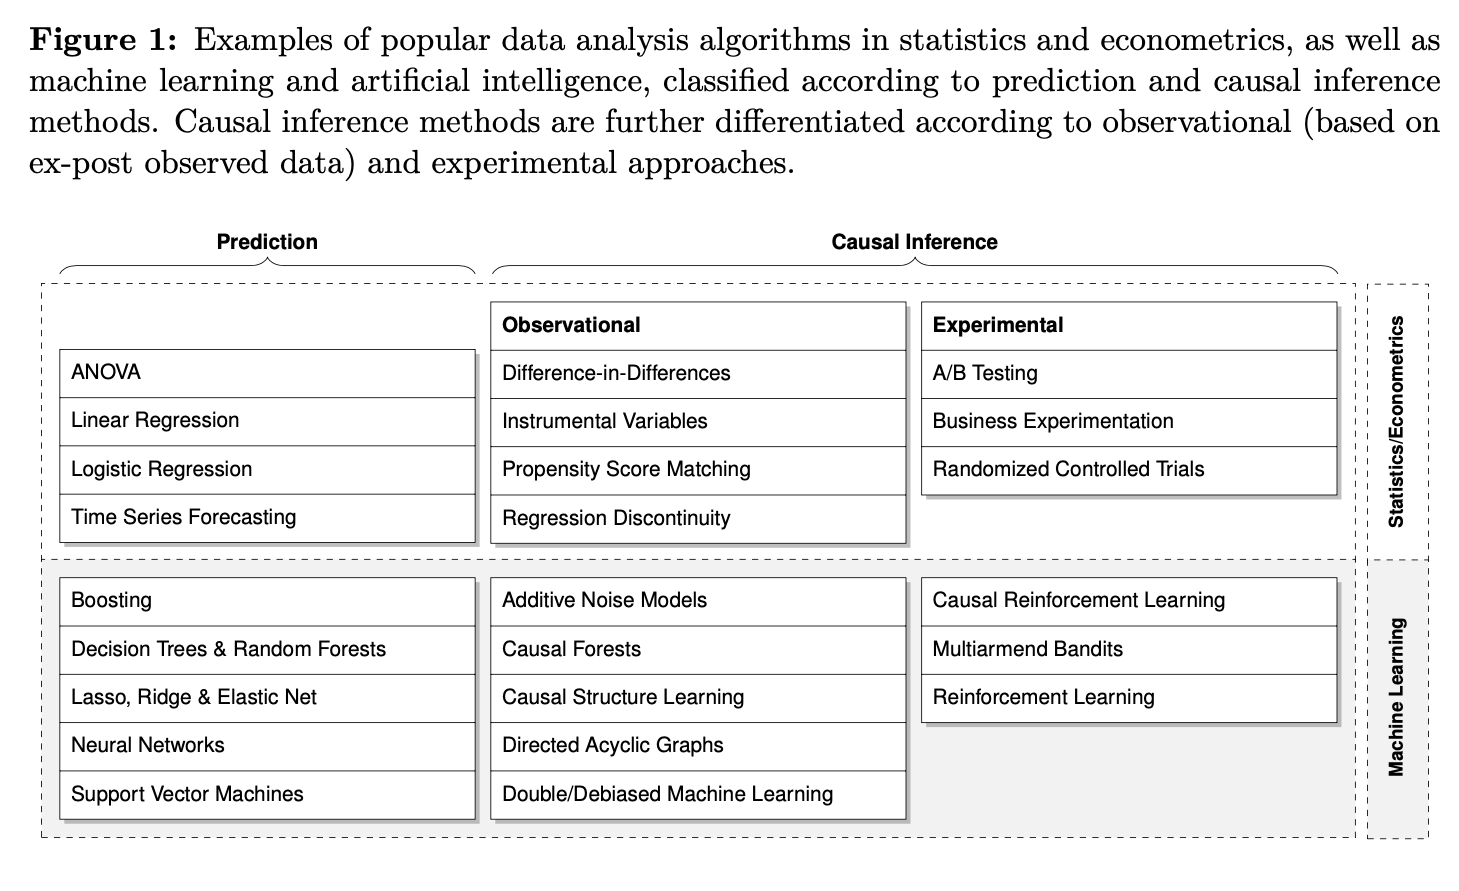
\includegraphics[scale=0.5,height=6.5cm, width=10cm]{./lecture_includes/prediction_causality.png}
\end{frame}

\begin{frame}{Causal Inference vs Prediction}

  \begin{columns}
    \column{0.48\linewidth}
    \centering
    \textbf{Traditional prediction}
    \begin{itemize}
      \item Traditional prediction seeks to detect patterns in data and fit functional relationships between variables with a high degree of accuracy
      \item ``Does this person have heart disease?'', ``How many books will I sell?''
      \item It is not predictions of what effect a choice will have, though
    \end{itemize}
    \column{0.48\linewidth}
    \centering
    \textbf{Causal inference}
    \begin{itemize}
      \item Causal inference is also a type of prediction, but it's a prediction of a \emph{counterfactual} associated with a particular \emph{choice taken}
      \item Causal inference takes that predicted (or imputed) counterfactual and constructs a causal effect that we hope tells us about a future in the event of a similar choice taken
    \end{itemize}
  \end{columns}
\end{frame}




\begin{frame}{Potential outcomes history}

\begin{itemize}

\item Causal inference is a scientific field within and across all major scientific categories focused on the epistemological foundations for believing one thing causes another
\item Core idea in causal inference is to distinguish between what is the true (``realized outcome'') versus what may have been possible had something been different (``counterfactual'')
\item Many people lay ownership to the following notation but it's broadly thought the mathematical notation comes from Jerzy Neyman's 1923 masters thesis, but you can find the ideas before him (e.g., John Stuart Mill, Ronald Fisher)
\item Most commonly associated today with Don Rubin, former chair of Harvard's stats department (now retired)

\end{itemize}

\end{frame}




\begin{frame}{Potential outcomes notation}
	
	\begin{itemize}
	\item Let the treatment be a binary variable: $$D_{i,t} =\begin{cases} 1 \text{ if in job training program $t$} \\ 0 \text{ if not in job training program at time $t$} \end{cases}$$where $i$ indexes an individual observation, such as a person

	\end{itemize}
\end{frame}

\begin{frame}{Potential outcomes notation}
	
	\begin{itemize}

	\item Potential outcomes: $$Y_{i,t}^j =\begin{cases} 1 \text{: wages at time $t$ if trained} \\ 0 \text{: wages at time $t$ if not trained} \end{cases}$$where $j$ indexes a counterfactual state of the world

	\end{itemize}
\end{frame}



\begin{frame}{Treatment effect definitions}


	\begin{block}{Individual treatment effect}
	    The individual treatment effect,  $\delta_i$, equals $Y_i^1-Y_i^0$
	\end{block}

Missing data problem:  I don't know my own counterfactual
	
\end{frame}


\begin{frame}{Conditional Average Treatment Effects}	
	\begin{block}{Average Treatment Effect on the Treated (ATT)}
	The average treatment effect on the treatment group is equal to the average treatment effect conditional on being a treatment group member:
		\begin{eqnarray*}
		E[\delta|D=1]&=&E[Y^1-Y^0|D=1] \nonumber \\
		&=&E[Y^1|D=1]-\textcolor{red}{E[Y^0|D=1]}
		\end{eqnarray*}
	\end{block}
	
	\bigskip

This is one of the most important policy parameters, if not the most important, and coincidentally it's also the parameter you get with synthetic control.  

	
\end{frame}




\section{Synthetic control and Modifications}

\subsection{Original synthetic control method}


\begin{frame}[plain]
	\begin{figure}
	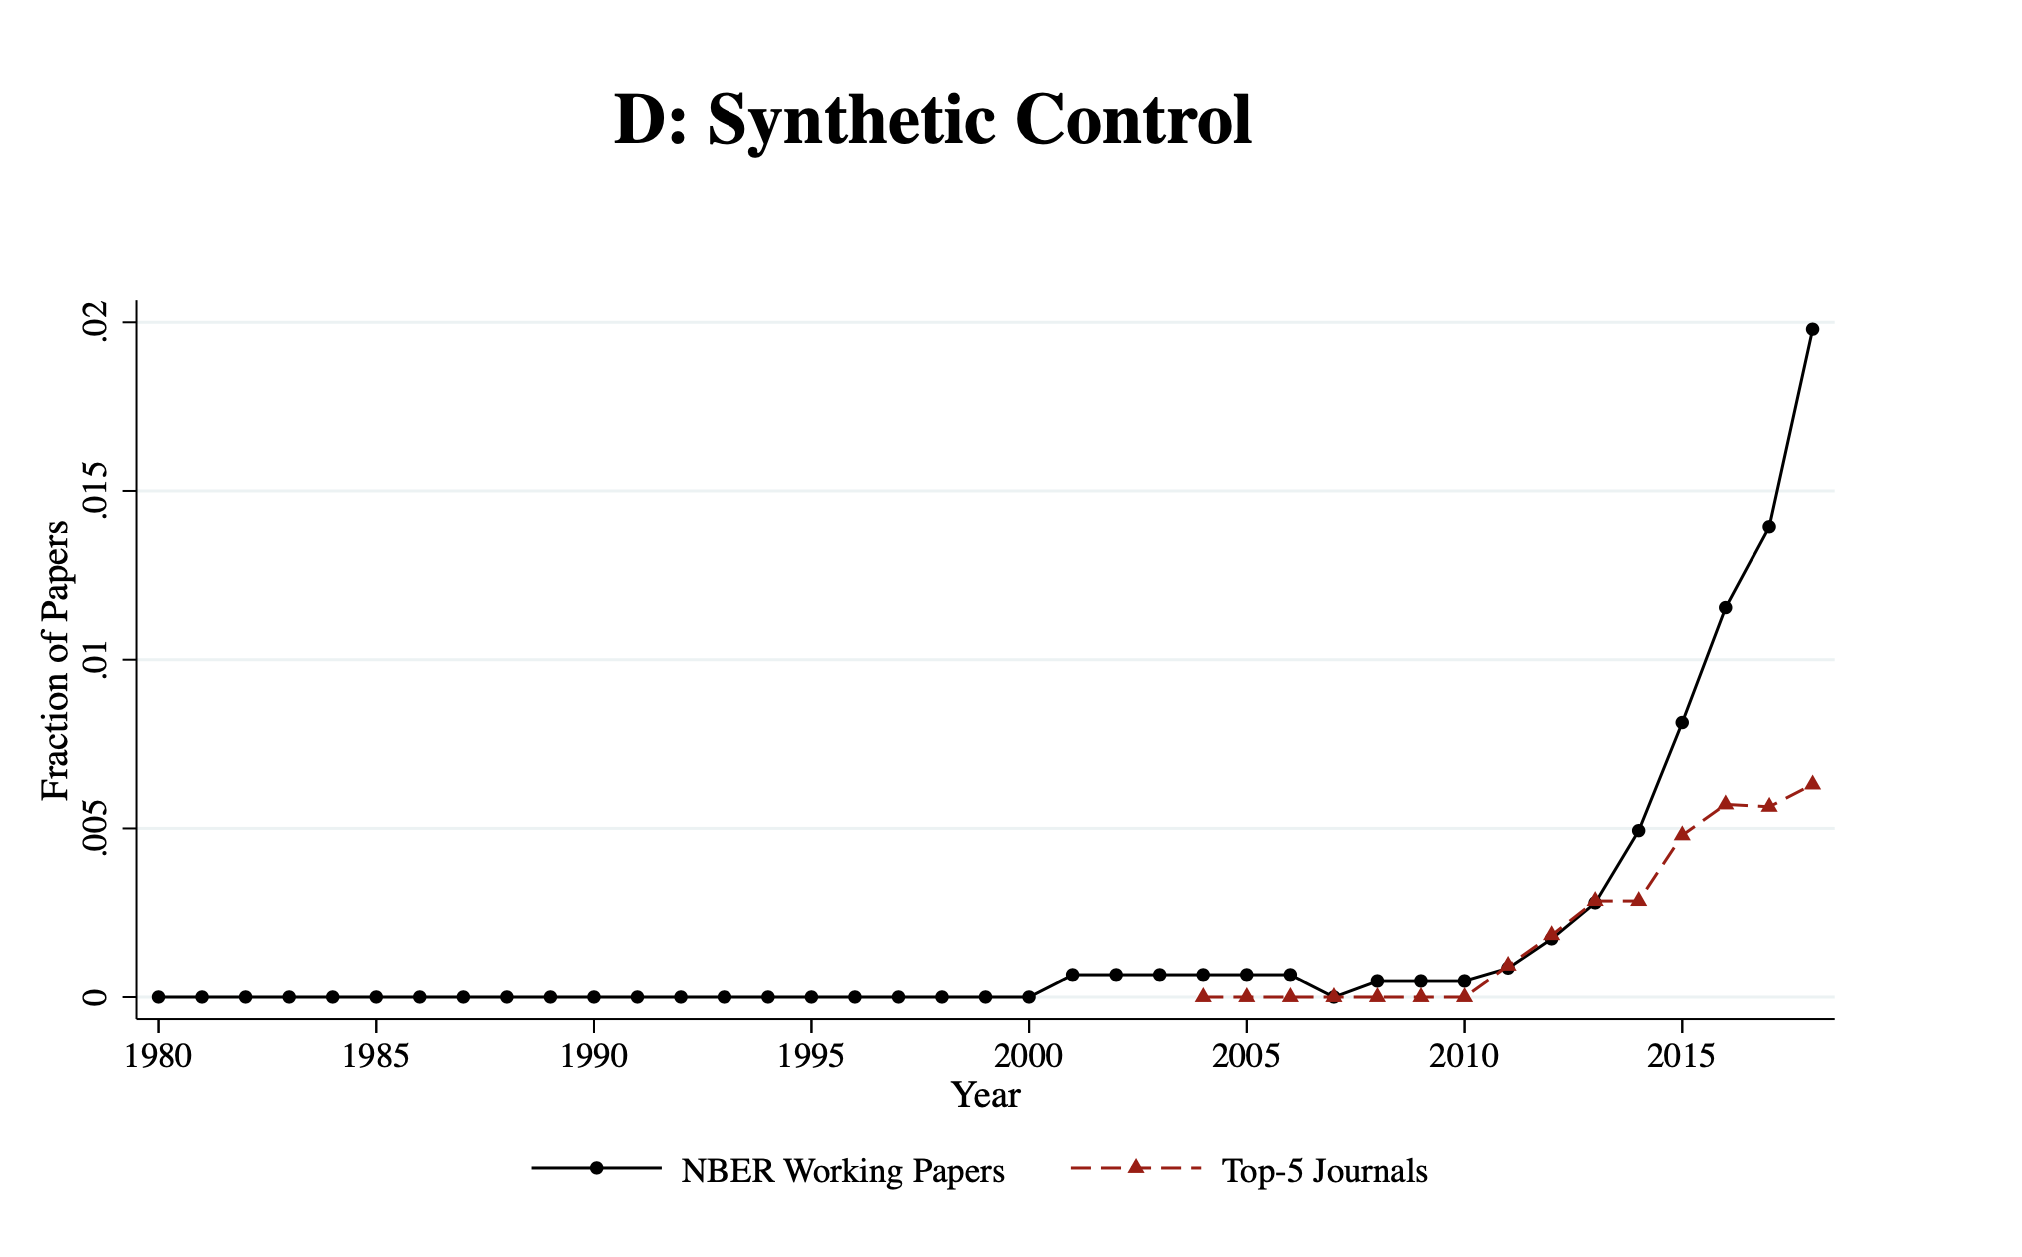
\includegraphics[scale=0.25]{./lecture_includes/currie_synth.png}
	\end{figure}
\end{frame}

\begin{frame}{What is synthetic control}
	
	\begin{itemize}
	\item Synthetic control has been called the most important innovation in causal inference of the last two decades by Athey and Imbens (2017)
	\item Originally designed for comparative case studies, but ongoing developments have extended it to multiple treated units, differential timing, bias adjustment and even modifications to difference-in-differences
	\item Methodologically synthetic control is at the frontier of ``causal panel models'' and we will try to build a ramp up to that frontier starting with the first method by Alberto Abadie and coauthors in 2003 and 2010
	\end{itemize}
\end{frame}
	
\begin{frame}{What is a comparative case study?}

\begin{itemize}
\item Comparative case studies compare a single aggregate unit (like a country) to another unit (like another country) to make statements about causal effects from aggregate policies or events
\item But the single treated unit can be any aggregate unit: a country, a state, school, firm, etc. 
\item Social scientists traditionally approached comparative case studies in one of two ways:
	\begin{enumerate}
	\item \textcolor{blue}{Qualitatively} (political science)
	\item \textcolor{red}{Quantitatively} (economics)
	\end{enumerate}
\end{itemize}

\end{frame}


\begin{frame}{\textcolor{blue}{Qualitative} comparative case studies}
	
	\begin{itemize}
	\item In \textcolor{blue}{qualitative} comparative case studies, the goal might be to reason \emph{inductively} the causal effects of events or characteristics of a single unit on some outcome, oftentimes through logic and historical analysis.  
		\begin{itemize}
		\item Classic example of comparative case study approach is Alexis de Toqueville's \underline{Democracy in America} (but he is regularly comparing the US to France)
		\end{itemize}
	\item Sometimes there may not be an explicit counterfactual, or if there is, it's not principled (subjective researcher decision)
	\item Quantitative claims about causal effects are unlikely -- de Toqueville's won't claim GDP per capita fell \$500 when compared against France
	\end{itemize}
\end{frame}

\begin{frame}{Traditional \textcolor{red}{quantitative} comparative case studies}

\begin{itemize}
	\item Traditional  \textcolor{red}{quantitative}  comparative case studies are explicitly causal designs in that there is a treatment and control, usually involving natural experiment on a single aggregate unit
	\item Comparison focuses on the the evolution of an aggregate outcome for the unit affected by the intervention to the evolution of the same \emph{ad hoc} aggregate control group (Card 1990; Card and Krueger 1994)
	\item It'll essentially be diff-in-diff, but it may not use the event study, and the point is the choice of controls is a subset of all possible controls
\end{itemize}

\end{frame}

\begin{frame}{Pros and cons}
	Pros:

		\begin{itemize}
		\item Takes advantage of policy interventions that take place at an aggregate level (which is common and so this is useful)
		\item Aggregate/macro data are often available (which may be all we have)
		\end{itemize}
\end{frame}

\begin{frame}{Pros and cons}
	Cons:

		\begin{itemize}
		\item Selection of control group is \emph{ad hoc} -- opens up researcher biases, even unconscious
		\item Standard errors do not reflect uncertainty about the ability of the control group to reproduce the counterfactual of interest
		\end{itemize}
\end{frame}


\begin{frame}{Description of the Mariel Boatlift}
	
	\begin{itemize}
	\item In 1980, Fidel Castro allowed anyone to leave Cuba so long as they did in the fall from the Mariel boat dock.
	\item The Mariel Boatlift brought 100,000 Cubans to Miami which increased the Miami labor force by 7\%
	\item Card (1990) uses the Mariel Boatlift as a natural experiment to measure the effect of a sudden influx of immigrants on unemployment among less-skilled natives
	\item His question was how do inflows of immigrants affect the wages and employment of natives in local US labor markets?
	\item Individual-level data on unemployment from the Current Population Survey (CPS) for Miami and comparison cities
	\end{itemize}
\end{frame}


\begin{frame}[plain]
	\begin{figure}
	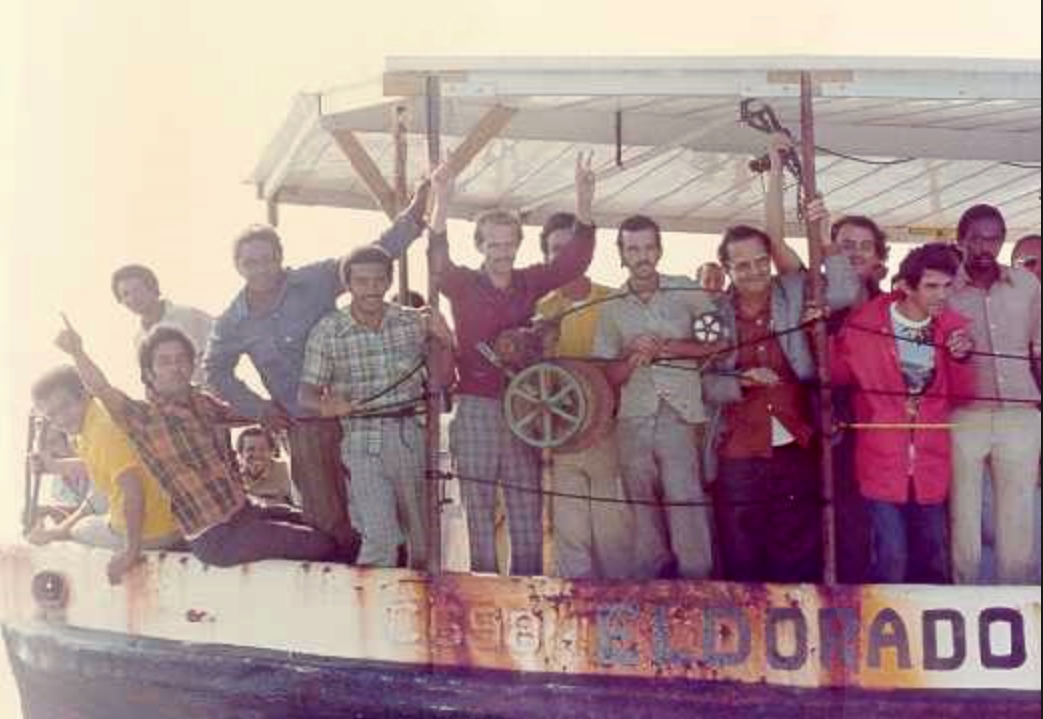
\includegraphics[scale=0.25]{./lecture_includes/boatlift2.png}
	\end{figure}
\end{frame}

\begin{frame}[plain]
	\begin{figure}
	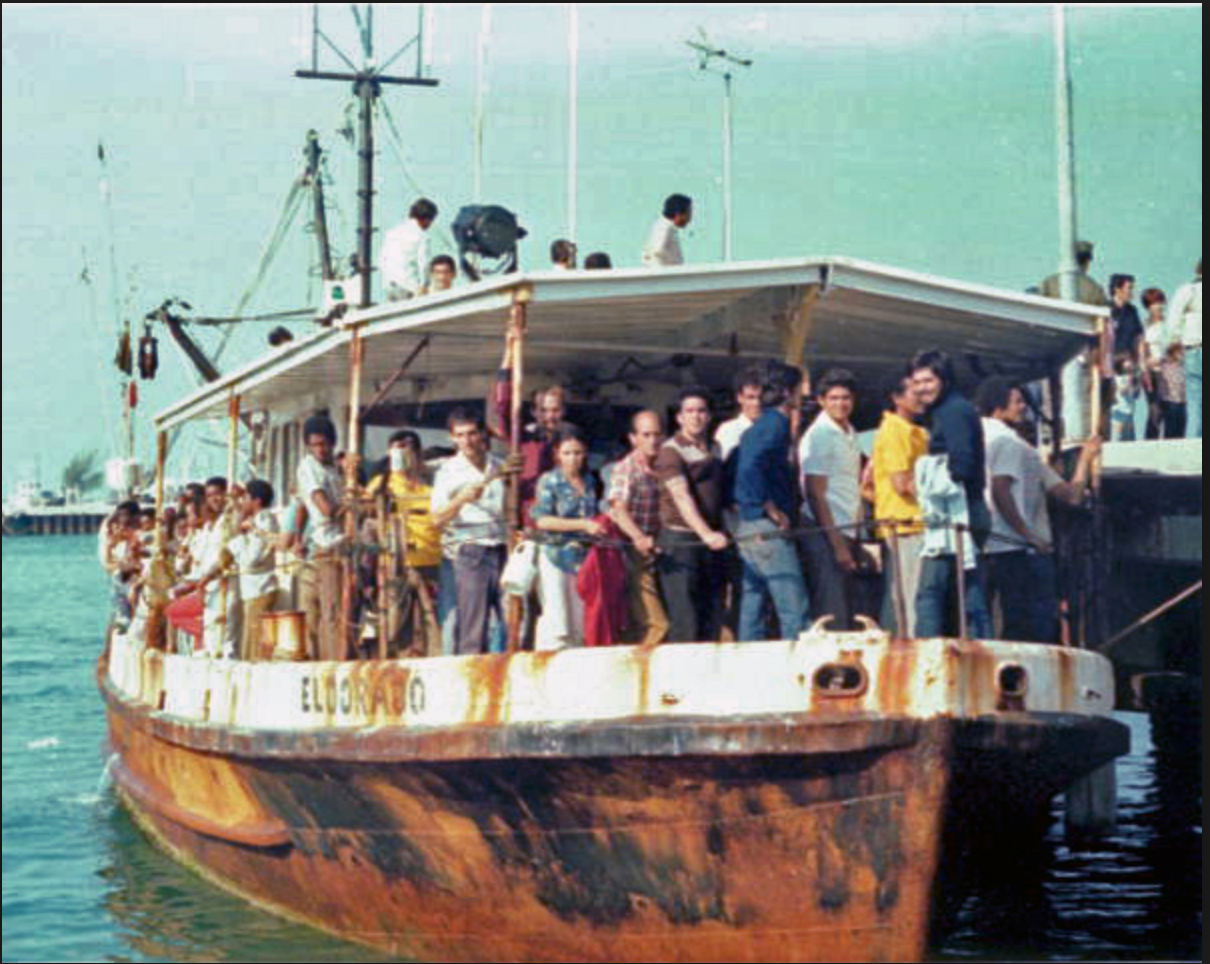
\includegraphics[scale=0.25]{./lecture_includes/boatlift3.png}
	\end{figure}
\end{frame}

\begin{frame}[plain]
	\begin{figure}
	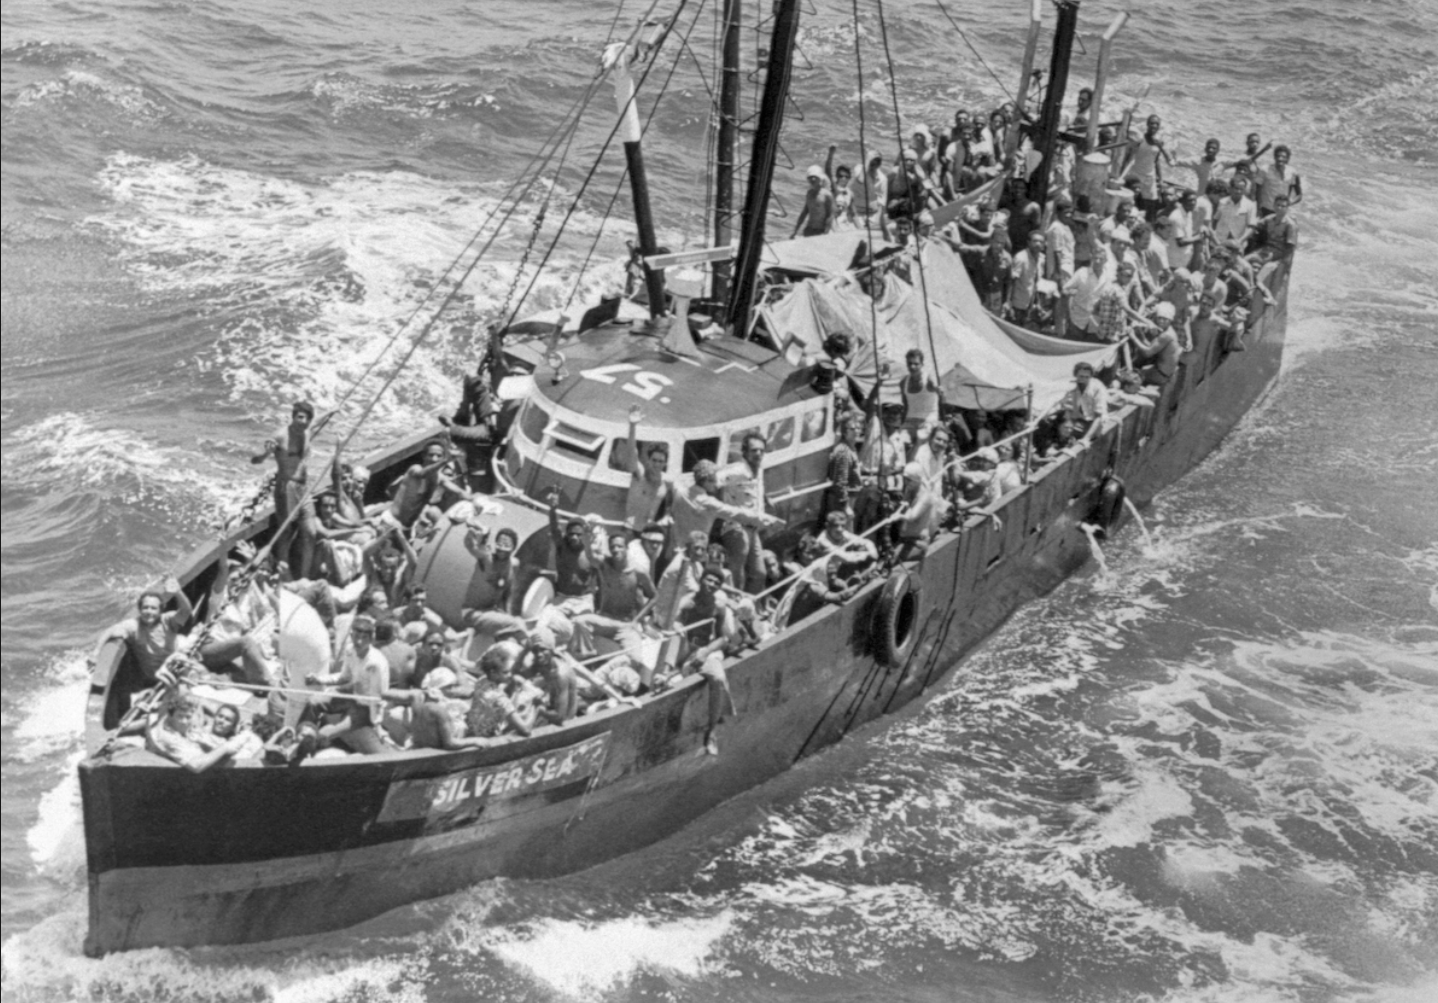
\includegraphics[scale=0.25]{./lecture_includes/boatlift4.png}
	\end{figure}
\end{frame}



\begin{frame}{Selecting control groups}

\begin{itemize}

\item His treatment group was low skill workers in Miami since that's where Cubans went
\item But which control group?
\item He chose Atlanta, Los Angeles, Houston, Tampa-St. Petersburg

\end{itemize}

\end{frame}



\begin{frame}{Why these four?}

	\begin{figure}
	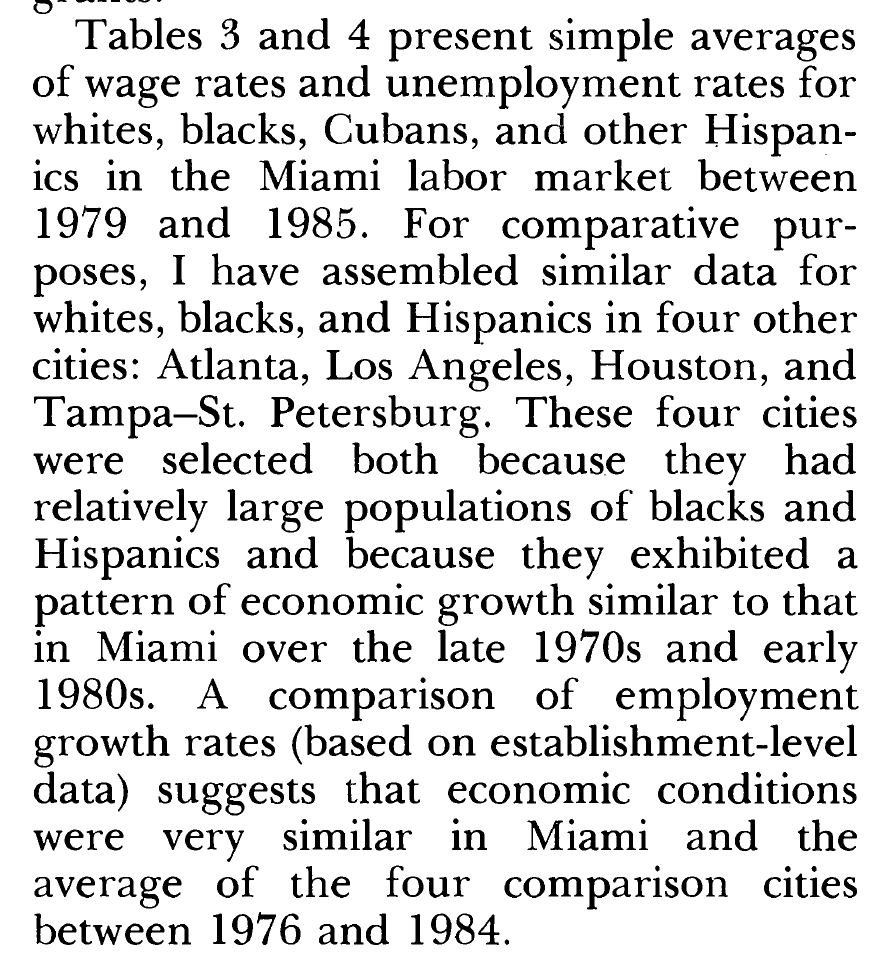
\includegraphics[scale=0.25]{./lecture_includes/card_illr.png}
	\end{figure}

\end{frame}

\begin{frame}{Diff-in-diff}
	
	\begin{figure}
	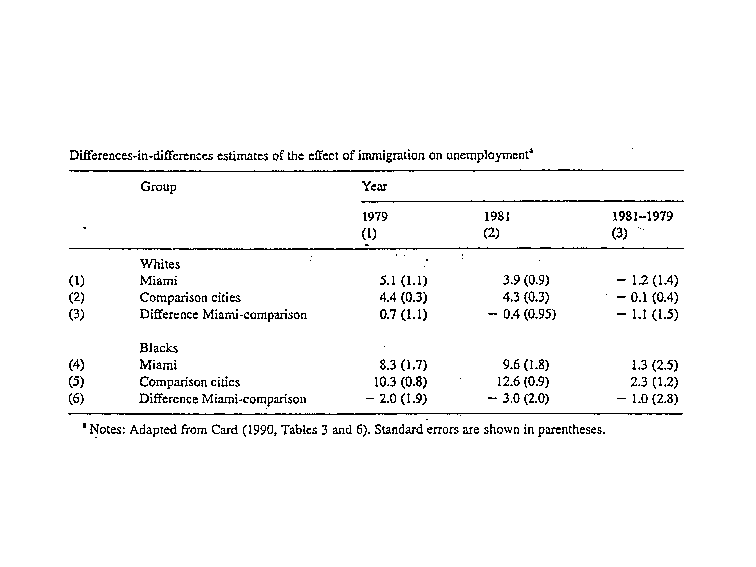
\includegraphics[scale=0.75]{./lecture_includes/abadie_2.pdf}
	\end{figure}
\end{frame}

\begin{frame}{Parallel trends}

\begin{itemize}
\item Card's analysis used diff-in-diff to estimate the impact of the Mariel boatlift on domestic labor markets
\item His estimate is unbiased if $\Delta E[Y^0]$ for the comparison cities approximates the counterfactual $\textcolor{violet-red}{\Delta E[Y^0]}$ for the treatment group
\item Card selected his controls based on a mixture of matching logic (e.g., covariates) and trend logic (e.g., employment growth) but does not report much
\item Black result would have been positive, too, were it not that the comparison cities growth was twice as large
\item Creates uncertainty about his null result -- was it no effect or was it the control group?
\end{itemize}

\end{frame}


\begin{frame}{Synthetic Control}
	
	\begin{itemize}
	\item Abadie and Gardeazabal (2003) introduced synthetic control in the AER in a study of a terrorist attack in Spain (Basque Country) on GDP
	\item Revisited again in a 2010 JASA with Diamond and Hainmueller, two political scientists who were PhD students at Harvard (more proofs and inference)
	\item Basic idea is to use a combination of comparison units as counterfactual for a treated unit where the units are chosen according to a data driven procedure
	\end{itemize}
\end{frame}


\begin{frame}{Researcher's objectives}

\begin{itemize}
	\item Synthetic control is a constrained minimization problem where the target goal is the minimization of a vector of squared gaps in pre-treatment characteristics
	\item Choice vector is an endogenous weights that are constant per control group unit over time and range from [0,1). 
	\item Our goal here is to reproduce the counterfactual of a treated unit by finding the combination of untreated units that best resembles the treated unit \emph{before} the intervention in terms of the values of $k$ relevant covariates (predictors of the outcome of interest)
	\item Method selects \emph{weighted average of all potential comparison units} that best resembles the characteristics of the treated unit(s) - called the ``synthetic control''
\end{itemize}

\end{frame}

\begin{frame}{Synthetic control method: advantages}
	
	\begin{itemize}
	\item ``Convex hull'' means synth is a non-negatively weighted average of donor pool units that on closely resemble the treatment group over time.
	\item Constraints on the model use non-negative weights which does not allow for extrapolation 
	\item Makes explicit the contribution of each comparison unit to the counterfactual 
	\item Formalizing the way comparison units are chosen has direct implications for inference
	\end{itemize}
\end{frame}




\begin{frame}{Notation and setup}
	
Suppose that we observe $J+1$ units in periods $1, 2, \dots, T$
		\begin{itemize}
		\item Unit ``one'' is exposed to the intervention of interest (that is, ``treated'') during periods $T_0+1, \dots, T$
		\item The remaining $J$ are an untreated reservoir of potential controls (a ``donor pool'')
		\end{itemize}	
\end{frame}


\begin{frame}{Potential outcomes notation}

		\begin{itemize}
		\item Let $Y_{it}^0$ be the outcome that would be observed for unit $i$ at time $t$ in the absence of the intervention
		\item Let $Y_{it}^1$ be the outcome that would be observed for unit $i$ at time $t$ if unit $i$ is exposed to the intervention in periods $T_0+1$ to $T$.
		\end{itemize}

\end{frame}

\begin{frame}{Group-time ATT with only one treated group}

Treatment effect parameter is defined as dynamic ATT where 

\begin{eqnarray*}
\delta_{1t}&=&Y_{1t}^1 - Y_{1t}^0 \\
&=& Y_{1t} - Y_{1t}^0 
\end{eqnarray*} for each post-treatment period, $t>T_0$ and $Y_{1t}$ is the outcome for unit one at time $t$. We will estimate $Y^0_{1t}$ using the $J$ units in the donor pool 

\end{frame}

\begin{frame}{Optimal weights}
	
	\begin{itemize}
	\item Let $W=(w_2, \dots, w_{J+1})'$ with $w_j\geq 0$ for $j=2, \dots, J+1$ and $w_2+\dots+w_{j+1}=1$. Each value of $W$ represents a potential synthetic control
	\item Let $X_1$ be a $(k\times 1)$ vector of pre-intervention characteristics for the treated unit.  Similarly, let $X_0$ be a $(k\times J)$ matrix which contains the same variables for the unaffected units.
	\item The vector $W^*=(w_2^*, \dots, w_{J+1}^*)'$ is chosen to minimize $||X_1-X_0W||$, subject to our weight constraints
	\end{itemize}
\end{frame}

\begin{frame}{Optimal weights differ by another weighting matrix}
	
Abadie, et al. consider $$||X_1 - X_0W||=\sqrt{(X_1-X_0W)'V(X_1-X_0W)}$$where $X_{jm}$ is the value of the $m$-th covariates for unit $j$ and $V$ is some $(k\times k)$ symmetric and positive semidefinite matrix

\end{frame}

\begin{frame}{More on the V matrix}

Typically, $V$ is diagonal with main diagonal $v_1, \dots, v_k$.  Then, the synthetic control weights $w_2^*, \dots, w_{J+1}^*$ minimize: $$\sum_{m=1}^k v_m \bigg(X_{1m} - \sum_{j=2}^{J+1}w_jX_{jm}\bigg)^2$$ where $v_m$ is a weight that reflects the relative importance that we assign to the $m$-th variable when we measure the discrepancy between the treated unit and the synthetic controls

\end{frame}

\begin{frame}{Choice of $V$ is critical}
	
		\begin{itemize}
		\item The synthetic control $W^*(V^*)$ is meant to reproduce the behavior of the outcome variable for the treated unit in the absence of the treatment
		\item Therefore, the $V^*$ weights directly shape $W^*$
		\end{itemize}
\end{frame}

\begin{frame}{Estimating the $V$ matrix}
	
 Choice of $v_1, \dots, v_k$ can be based on
		\begin{itemize}
		\item Assess the predictive power of the covariates using regression
		\item Subjectively assess the predictive power of each of the covariates, or calibration inspecting how different values for $v_1, \dots, v_k$ affect the discrepancies between the treated unit and the synthetic control
		\item Minimize mean square prediction error (MSPE) for the pre-treatment period (default):
			\begin{eqnarray*}
			\sum_{t=1}^{T_0} \bigg(Y_{1t} - \sum_{j=2}^J w_j^*(V^*)Y_{jt} \bigg)^2
			\end{eqnarray*}
		\end{itemize}
\end{frame}

\begin{frame}{Cross validation}

\begin{itemize}
		\item Divide the pre-treatment period into an initial \textbf{training} period and a subsequent \textbf{validation} period
		\item For any given $V$, calculate $W^*(V)$ in the training period.
		\item Minimize the MSPE of $W^*(V)$ in the validation period
\end{itemize}

\end{frame}



\begin{frame}{Example: California's Proposition 99}
	
	\begin{itemize}
	\item In 1988, California first passed comprehensive tobacco control legislation:
		\begin{itemize}
		\item increased cigarette tax by 25 cents/pack
		\item earmarked tax revenues to health and anti-smoking budgets
		\item funded anti-smoking media campaigns
		\item spurred clean-air ordinances throughout the state
		\item produced more than \$100 million per year in anti-tobacco projects
		\end{itemize}
	\item Other states that subsequently passed control programs are excluded from donor pool of controls (AK, AZ, FL, HI, MA, MD, MI, NJ, OR, WA, DC)
	\end{itemize}
\end{frame}

\begin{frame}{Cigarette Consumption: CA and the Rest of the US}
	
	\begin{figure}
	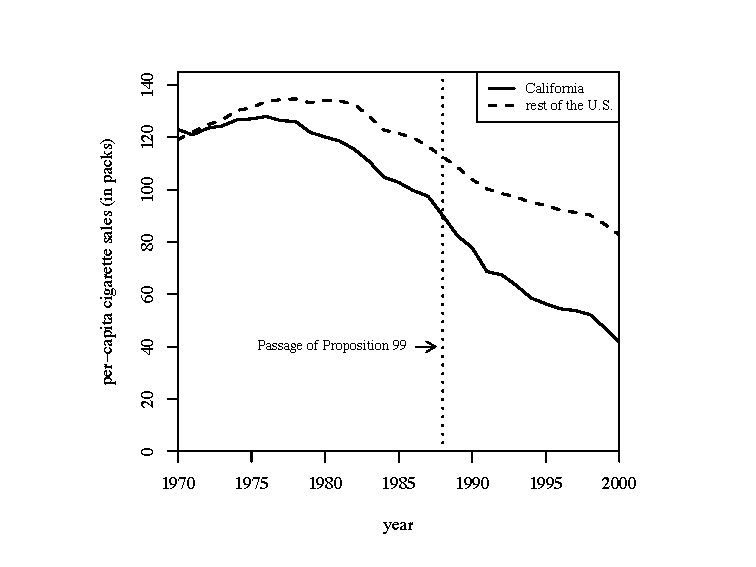
\includegraphics[scale=0.75]{./lecture_includes/abadie_3.pdf}
	\end{figure}
\end{frame}

\begin{frame}{Cigarette Consumption: CA and synthetic CA}
	
	\begin{figure}
	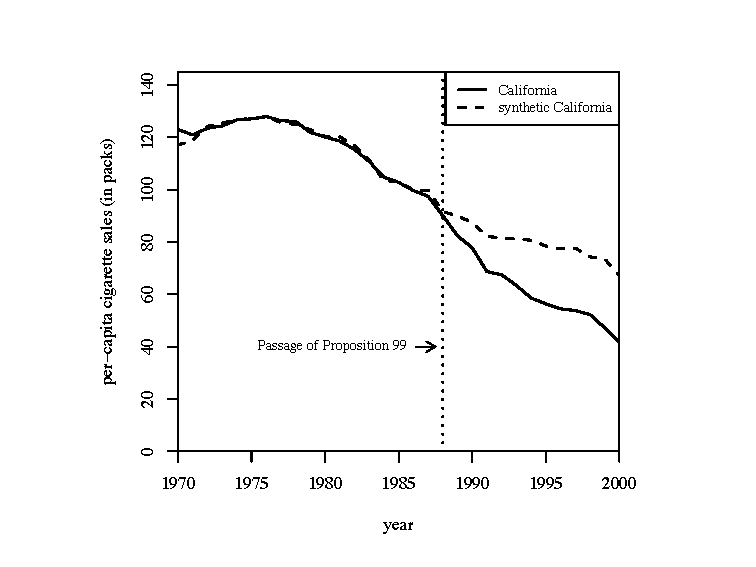
\includegraphics[scale=0.75]{./lecture_includes/abadie_4.pdf}
	\end{figure}
\end{frame}

\begin{frame}{Sparsity and Synthetic Control Weights}
	\begin{figure}
	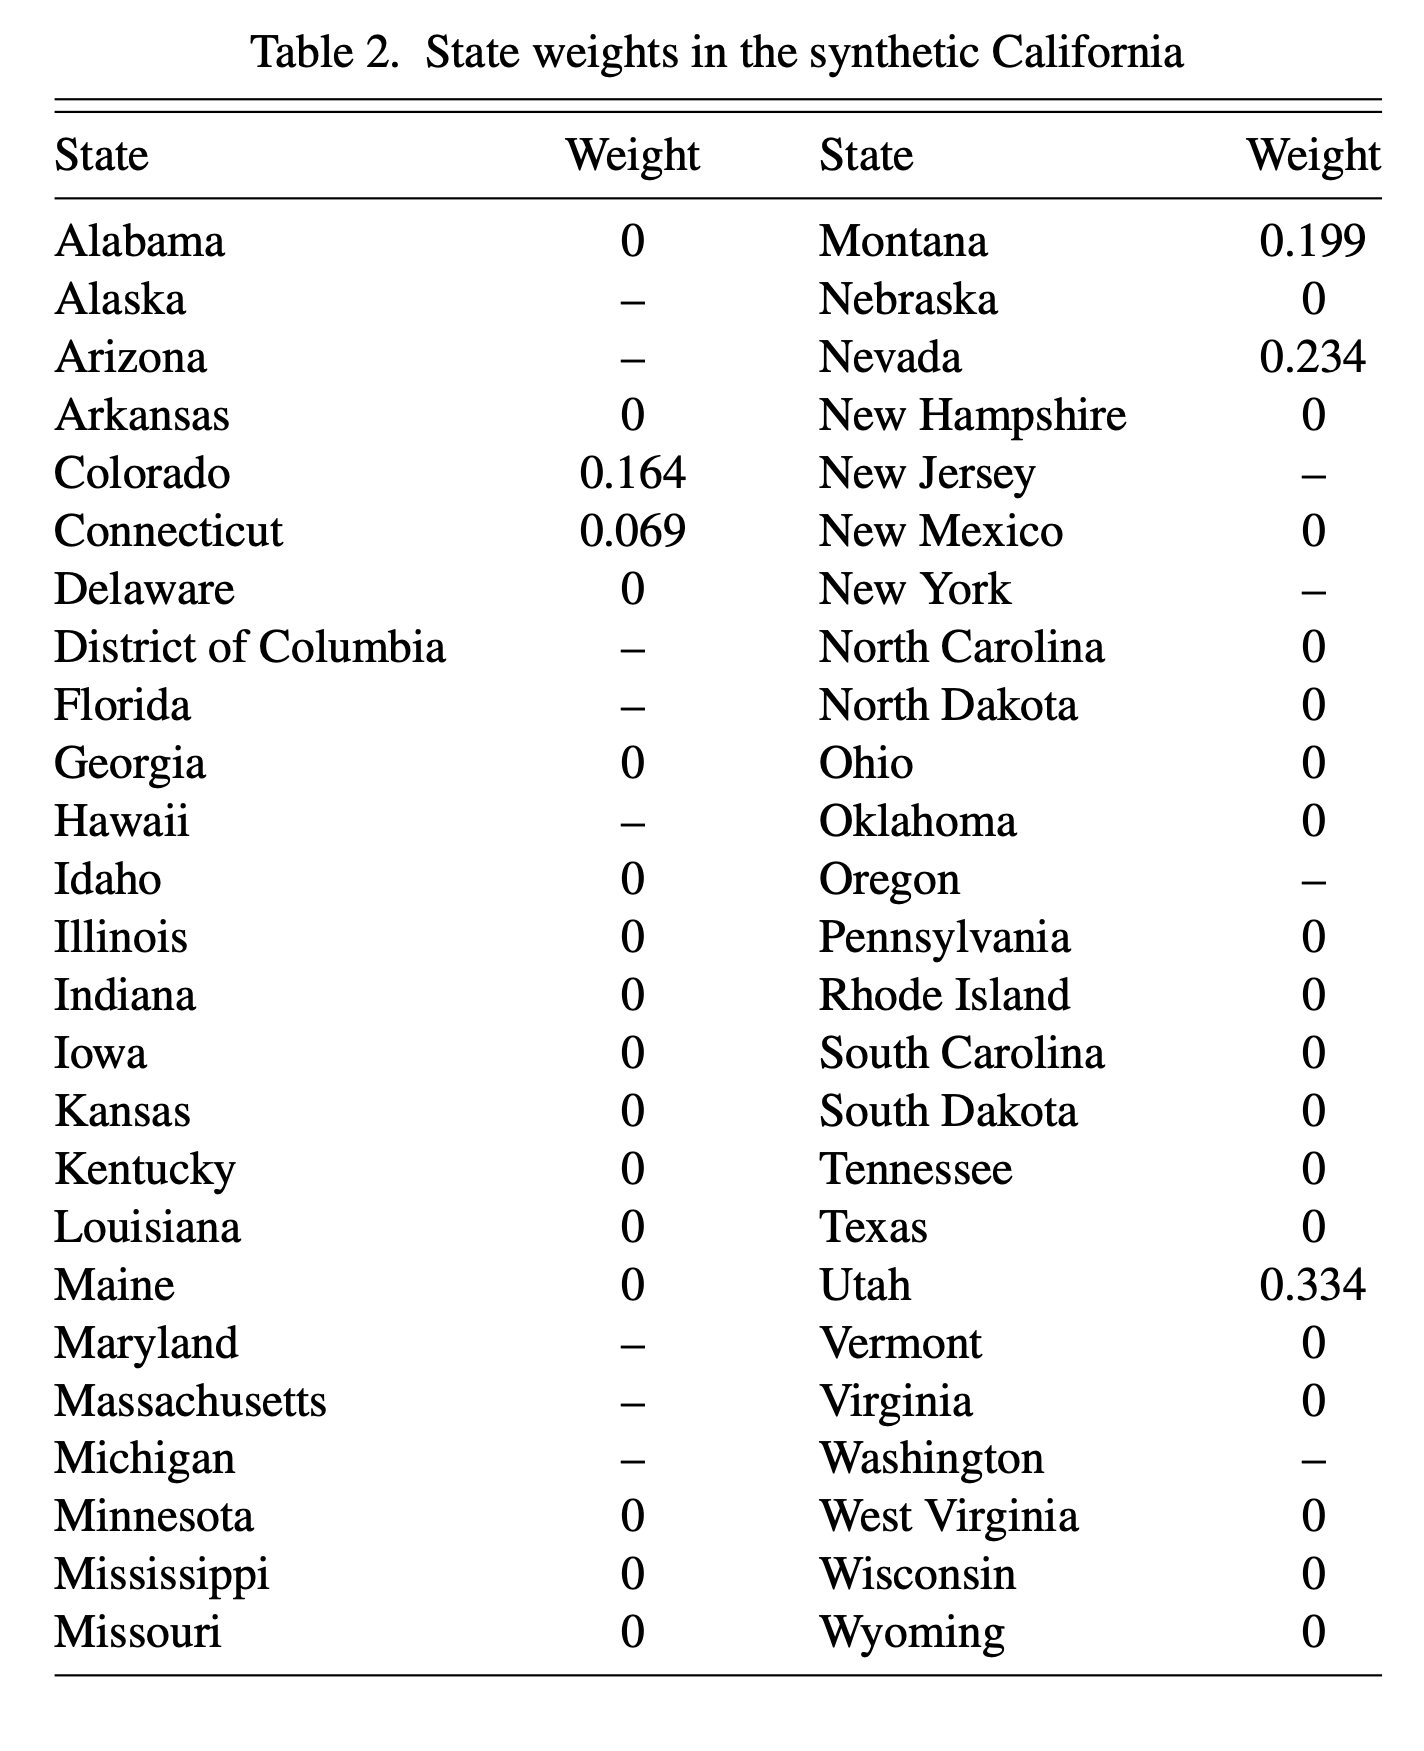
\includegraphics[scale=0.25]{./lecture_includes/synth_smoking_table2.png}
	\end{figure}
\end{frame}



\begin{frame}{Predictor Means: Actual vs. Synthetic California}
	
	\begin{figure}
	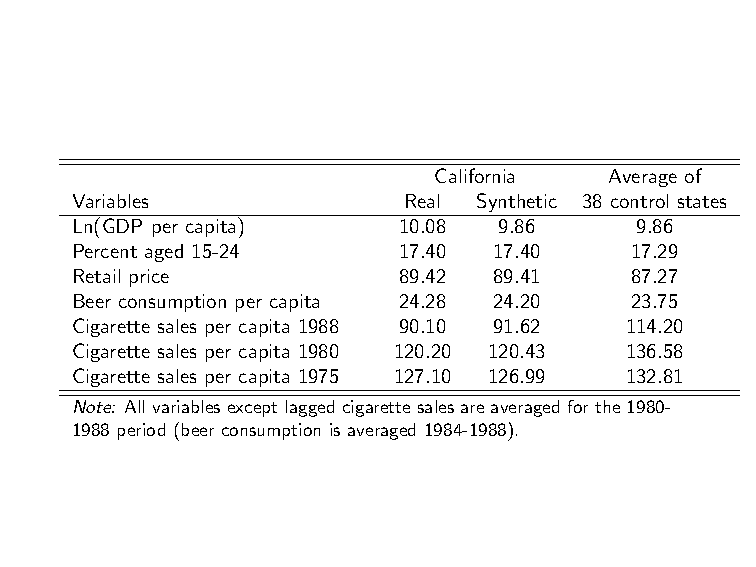
\includegraphics[scale=0.75]{./lecture_includes/abadie_5.pdf}
	\end{figure}
\end{frame}

\begin{frame}{Smoking Gap between CA and synthetic CA}
	
	\begin{figure}
	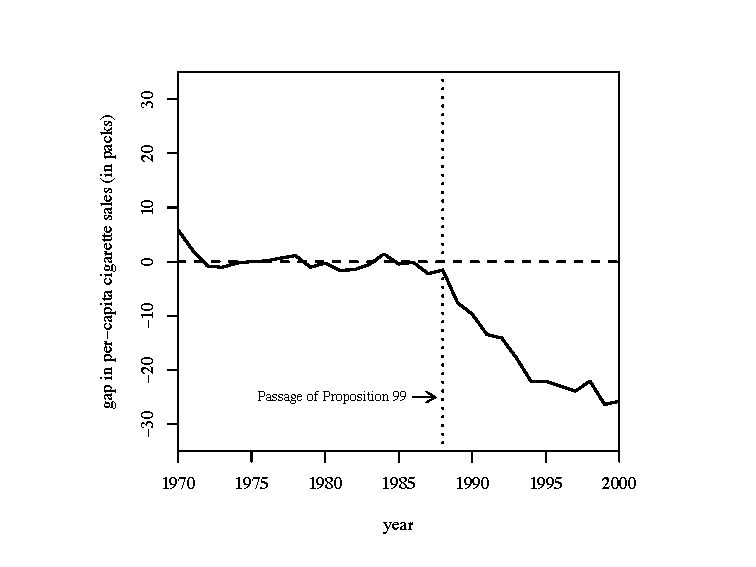
\includegraphics[scale=0.75]{./lecture_includes/abadie_6.pdf}
	\end{figure}
\end{frame}

\begin{frame}{Inference}
	
	\begin{itemize}
	\item To assess significance, we calculate exact p-values under Fisher's sharp null using a test statistic equal to after to before ratio of RMSPE
	\item Exact p-value method
		\begin{itemize}
		\item Iteratively apply the synthetic method to each country/state in the donor pool and obtain a distribution of placebo effects
		\item Compare the gap (RMSPE) for California to the distribution of the placebo gaps. For example the post-Prop. 99 RMSPE is: 
			\begin{eqnarray*}
			RMSPE = \bigg(\frac{1}{T-T_0} \sum_{t=T_0+1}^T \bigg(Y_{1t} - \sum_{j=2}^{J+1} w_j^* Y_{jt}\bigg)^2 \bigg)^{\frac{1}{2}}
			\end{eqnarray*}and the exact p-value is the treatment unit rank divided by $J$
		\end{itemize}
	\end{itemize}
\end{frame}

\begin{frame}{Smoking Gap for CA and 38 control states}
	
	\begin{figure}
	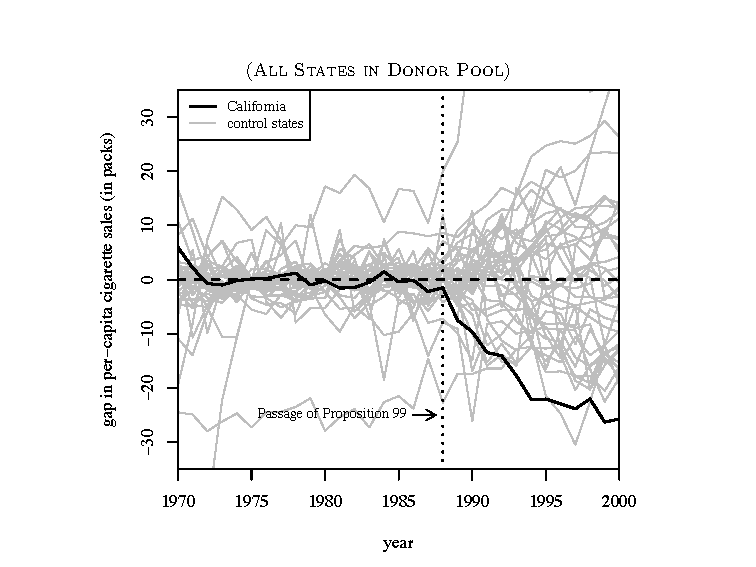
\includegraphics[scale=0.75]{./lecture_includes/abadie_7.pdf}
	\end{figure}
\end{frame}

\begin{frame}{Smoking Gap for CA and 34 control states}
	
	\begin{figure}
	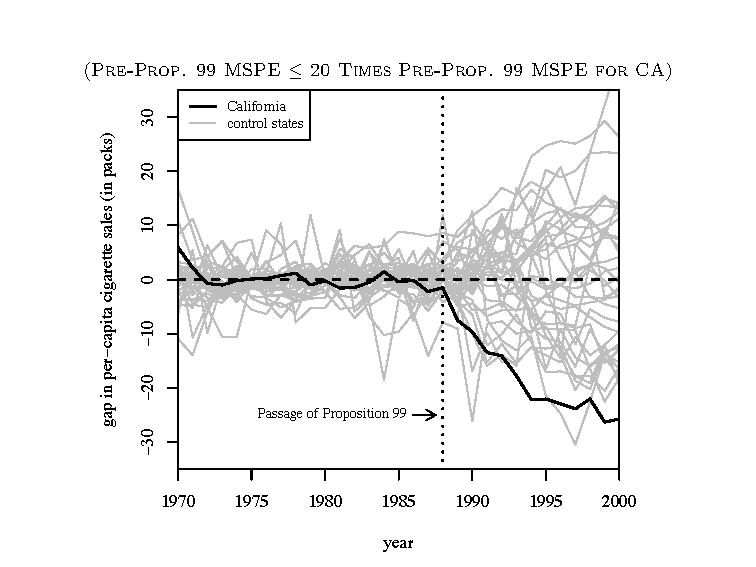
\includegraphics[scale=0.75]{./lecture_includes/abadie_8.pdf}
	\end{figure}
\end{frame}

\begin{frame}{Smoking Gap for CA and 29 control states}
	
	\begin{figure}
	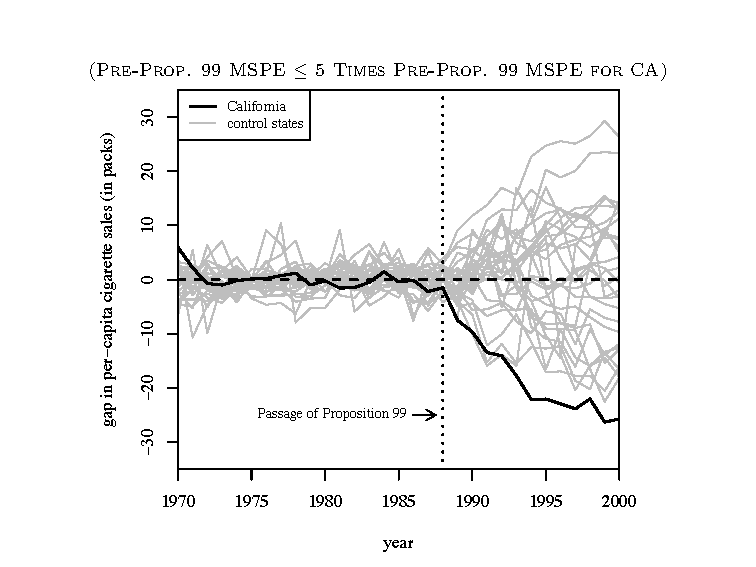
\includegraphics[scale=0.75]{./lecture_includes/abadie_9.pdf}
	\end{figure}
\end{frame}

\begin{frame}{Smoking Gap for CA and 19 control states}
	
	\begin{figure}
	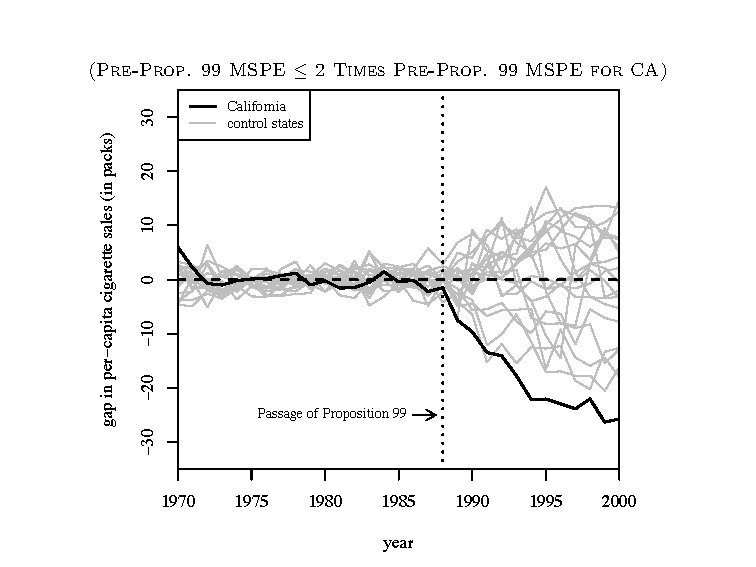
\includegraphics[scale=0.75]{./lecture_includes/abadie_10.pdf}
	\end{figure}
\end{frame}

\begin{frame}{Ratio Post-Prop. 99 RMSPE to Pre-Prop. 99 RMSPE}

	\begin{figure}
	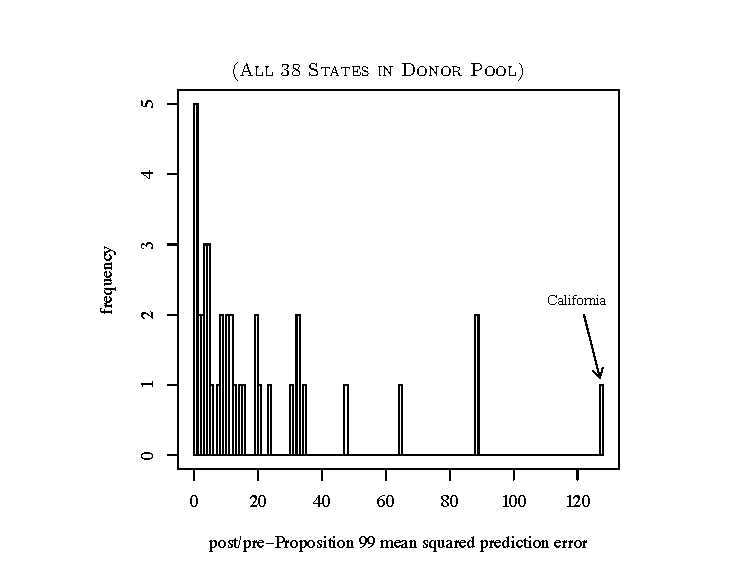
\includegraphics[scale=0.75]{./lecture_includes/abadie_11.pdf}
	\end{figure}
\end{frame}




\begin{frame}{Coding exercise}
	
	\begin{itemize}
	\item The US has the highest prison population of any OECD country in the world 
	\item 2.1 million are currently incarcerated in US federal and state prisons and county jails
	\item Another 4.75 million are on parole
	\item From the early 1970s to the present, incarceration and prison admission rates quintupled in size
	\end{itemize}
\end{frame}



\begin{frame}[plain]

\begin{figure}
\includegraphics[scale=0.5]{./lecture_includes/cook2010.pdf}
\end{figure}
\end{frame}


\begin{frame}{Prison constraints}

	
	\begin{itemize}
	\item Prisons are and have been at capacity for a long time so growth in imprisonment would bite on state corrections
	\item Managing increased flows can only be solved by the following:
		\begin{itemize}
		\item Prison construction
		\item Overcrowding
		\item Paroles
		\end{itemize}
	\item Texas chooses overcrowding
	\end{itemize}
\end{frame}



\begin{frame}{Ruiz v. Estelle 1980}

	
	\begin{itemize}
		\item Class action lawsuit against TX Dept of Corrections (Estelle, warden). 
		\item TDC lost.  Lengthy period of appeals and legal decrees.  
		\item Lengthy period of time relying on paroles to manage flows
	\end{itemize}
\end{frame}

\begin{frame}[plain]
  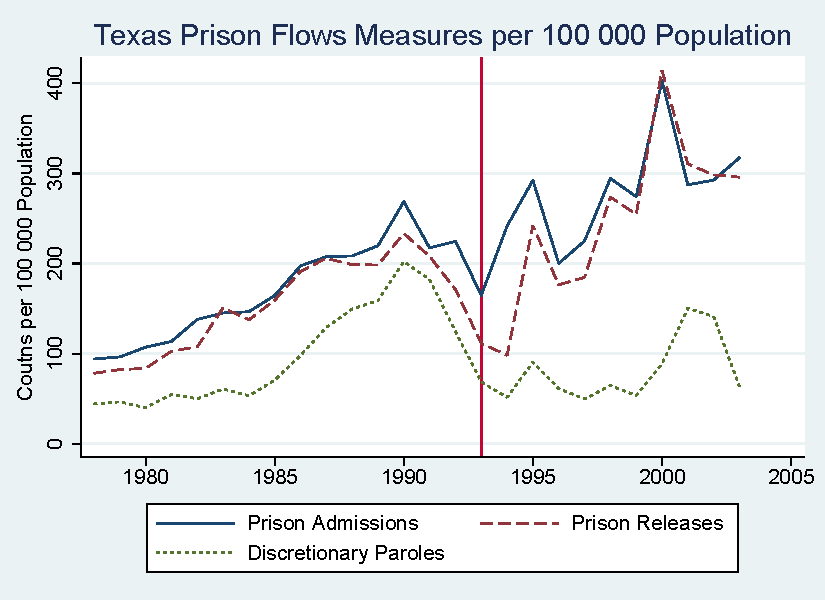
\includegraphics[scale=0.8]{./lecture_includes/flow_rate_figure.pdf}
\end{frame}

\begin{frame}{Texas prison boom}

Governor Ann Richards (D) 1991-1995
		\begin{itemize}
		\item Operation prison capacity increased 30-35\% in 1993, 1994 and 1995. 
		\item Prison capacity increased from 55,000 in 1992 to 130,000 in 1995.  
		\item Building of new prisons (private and public)
		\end{itemize} 
\end{frame}


\begin{frame}[shrink=30,plain]

\begin{figure}
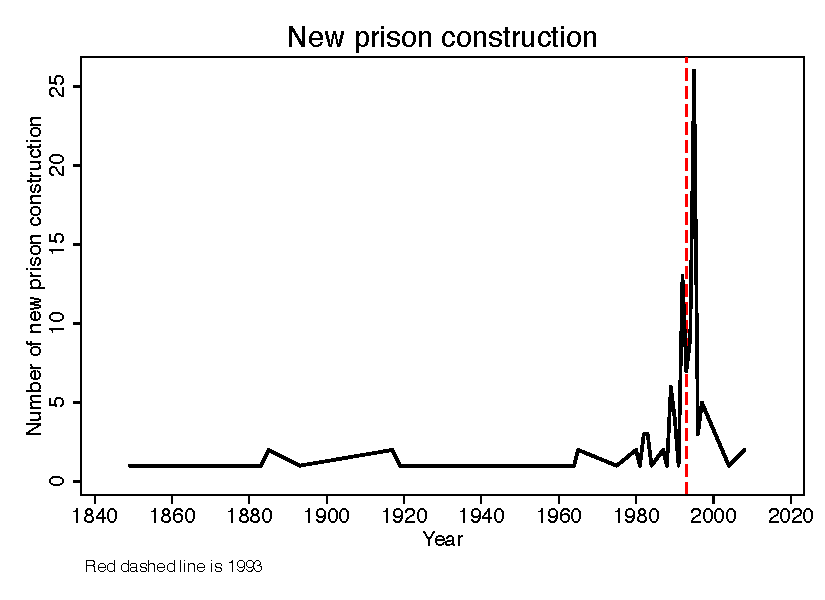
\includegraphics{./lecture_includes/tdcj.pdf}
\end{figure}
\end{frame}


\begin{frame}[shrink=30,plain]
\begin{figure}
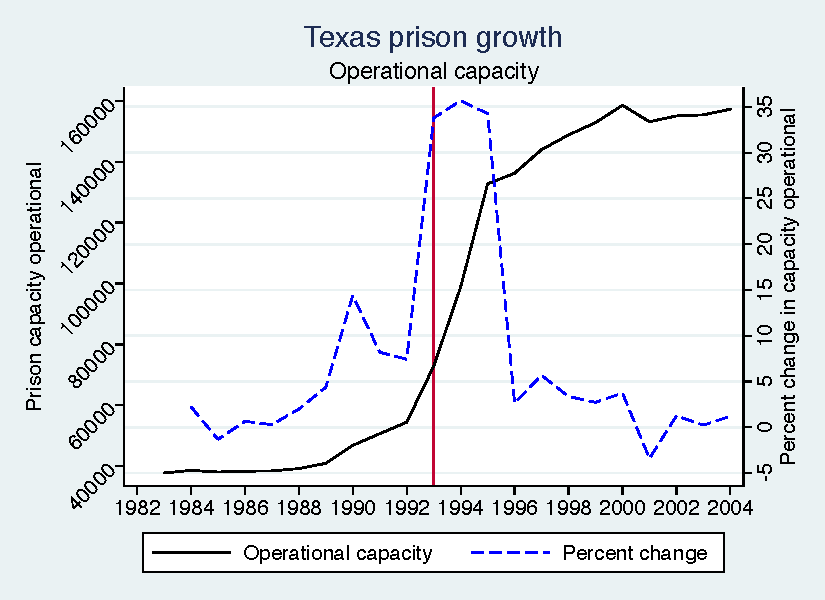
\includegraphics{./lecture_includes/capacity_operational_texas.pdf}
\end{figure}
\end{frame}



\begin{frame}[shrink=30,plain]

\begin{figure}
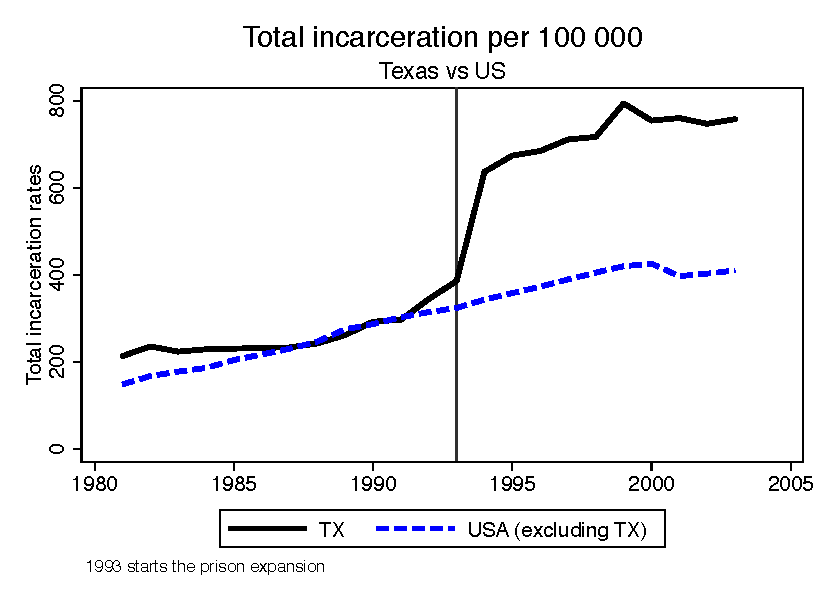
\includegraphics{./lecture_includes/total_incarceration.pdf}
\end{figure}
\end{frame}

\begin{frame}[shrink=30,plain]

\begin{figure}
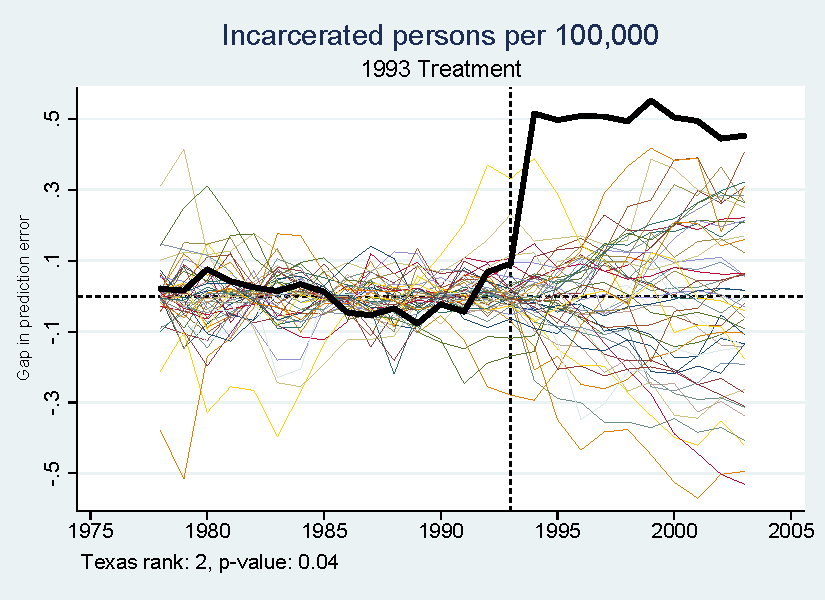
\includegraphics{./lecture_includes/synth_placebo_totalincarceration1993.pdf}
\end{figure}
\end{frame}


\begin{frame}{Coding together}

\begin{itemize}
\item Let's go to Mixtape Sessions repository now into /Labs/Texas 
\item I'll walk us through the Stata and R code so you understand the syntax and underlying logic
\item But then I have us a practice assignment 
\end{itemize}

\end{frame}


\begin{frame}{Avoiding Cherry Picking: Subway franchise and Scandal}

	\begin{figure}
	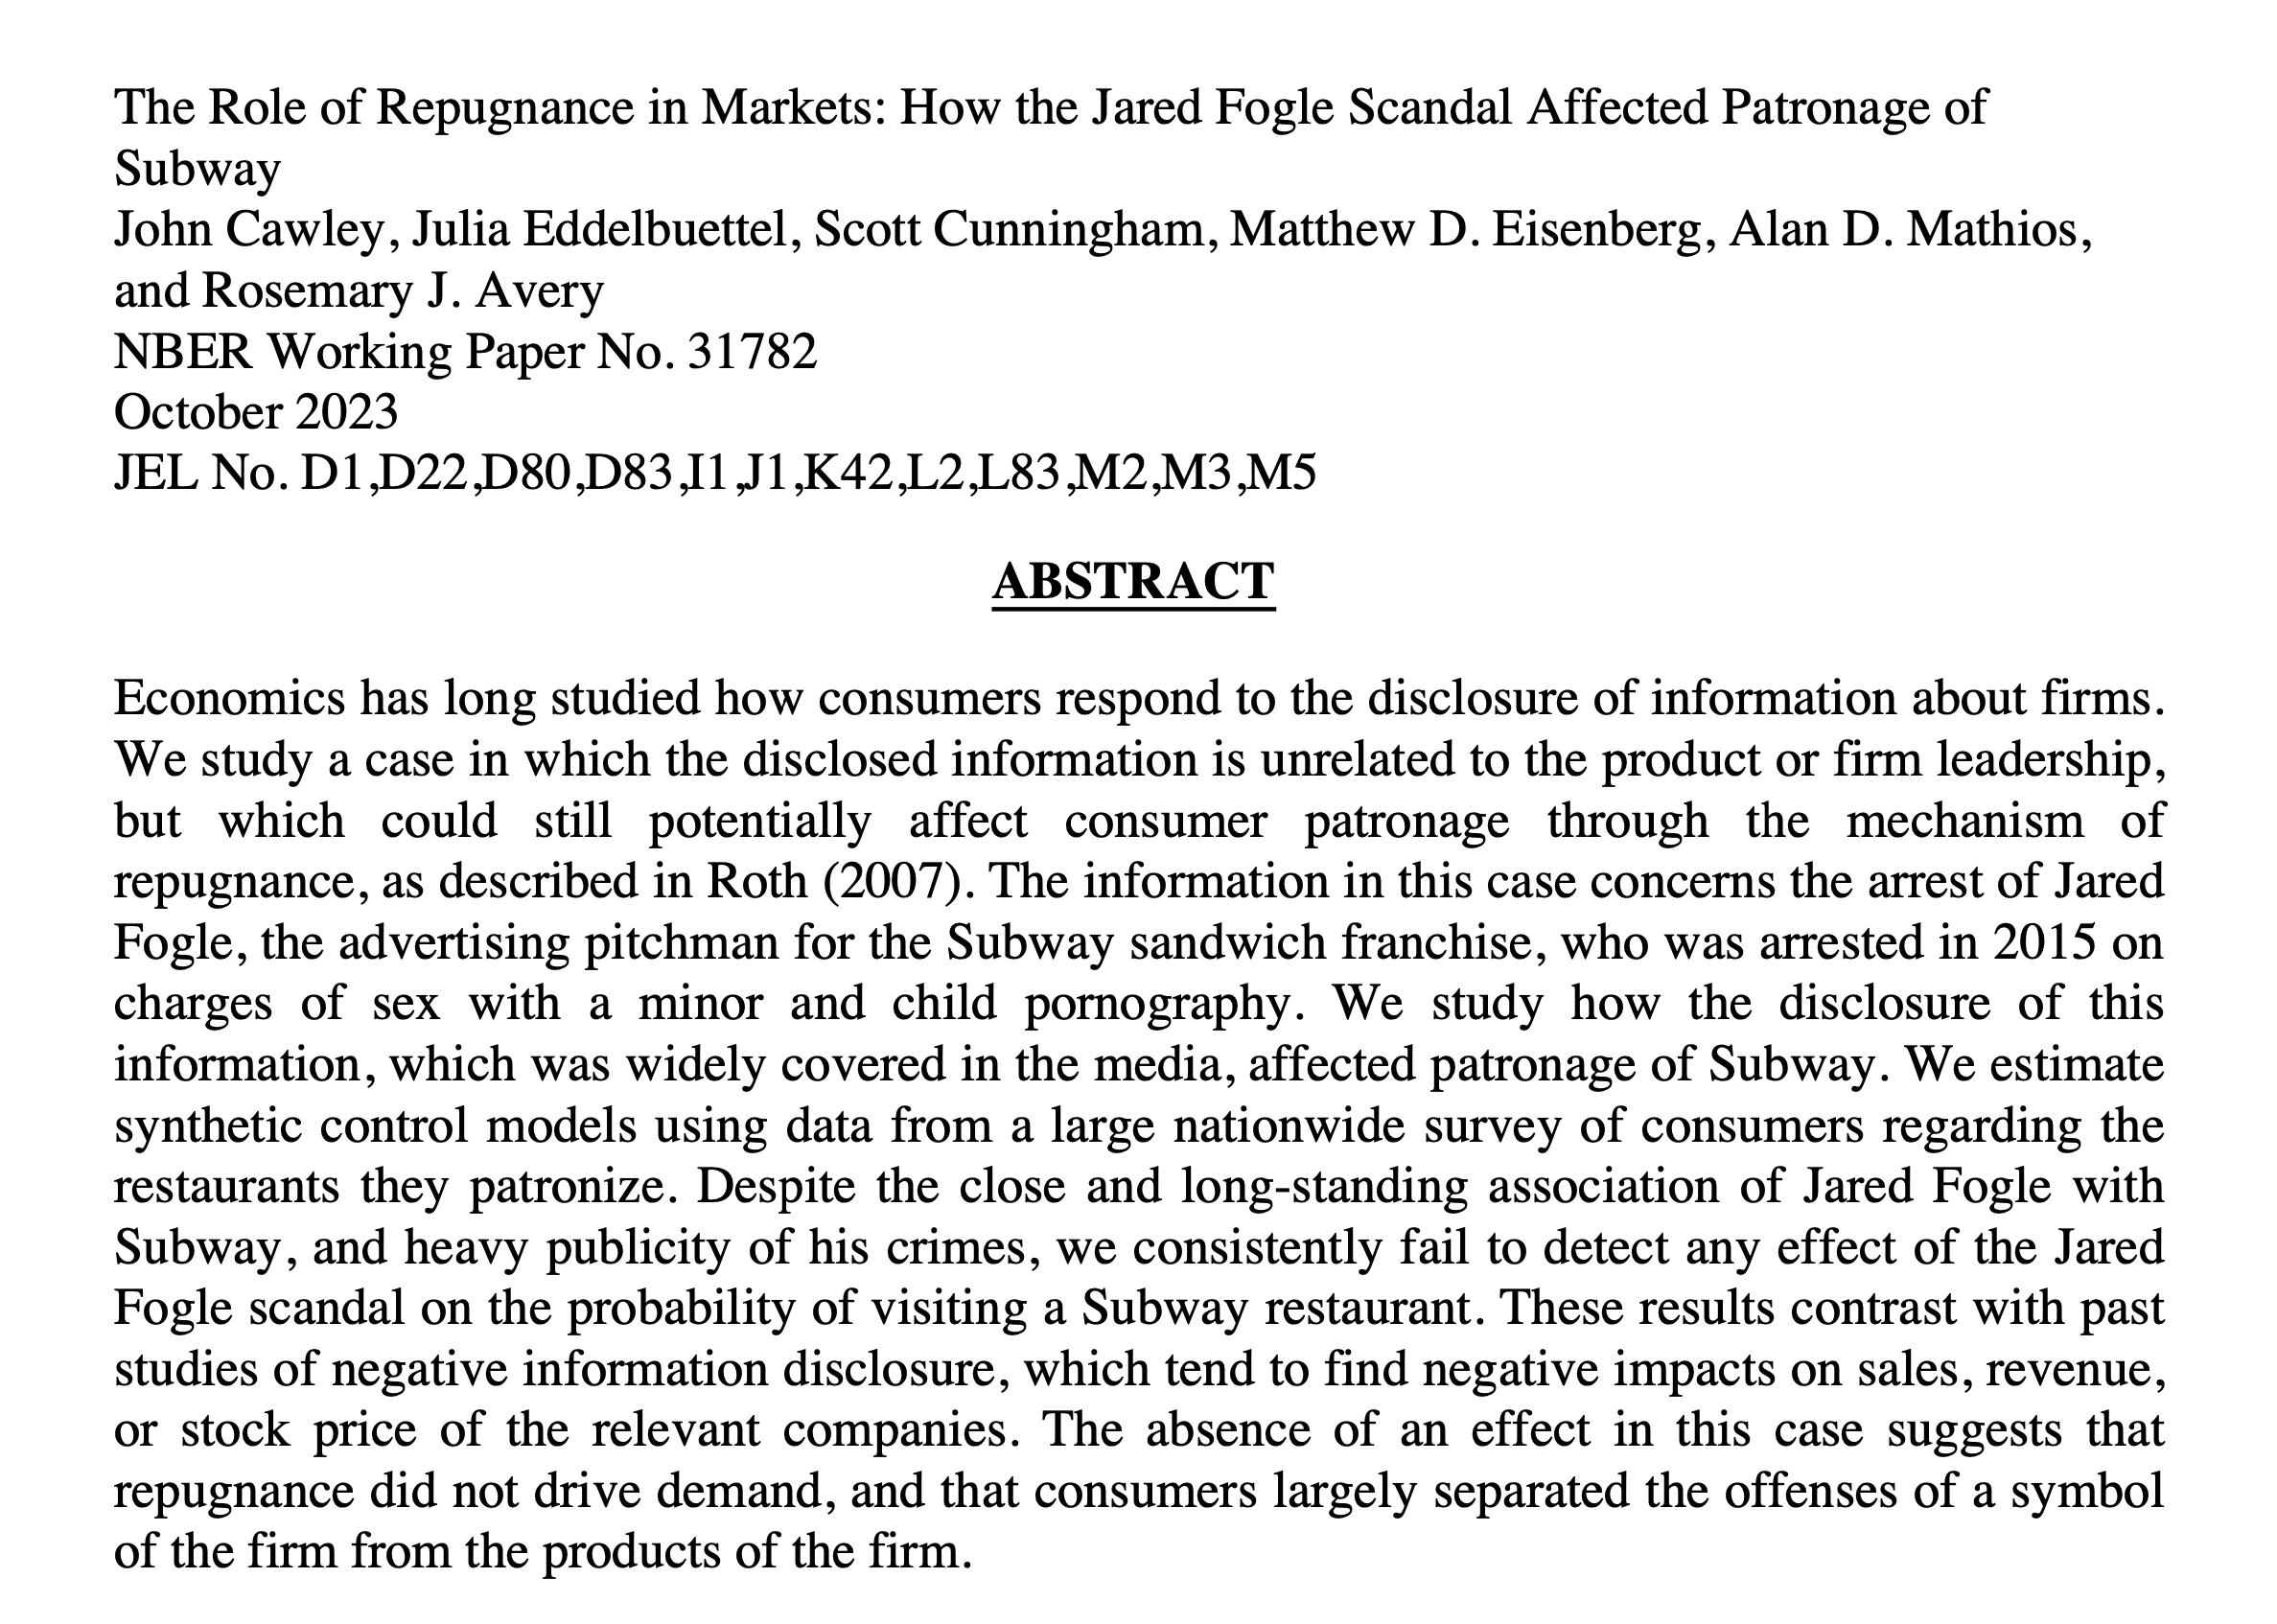
\includegraphics[scale=0.25]{./lecture_includes/subway_8.png}
	\end{figure}

\end{frame}

\begin{frame}{Subway franchise and Scandal}

	\begin{figure}
	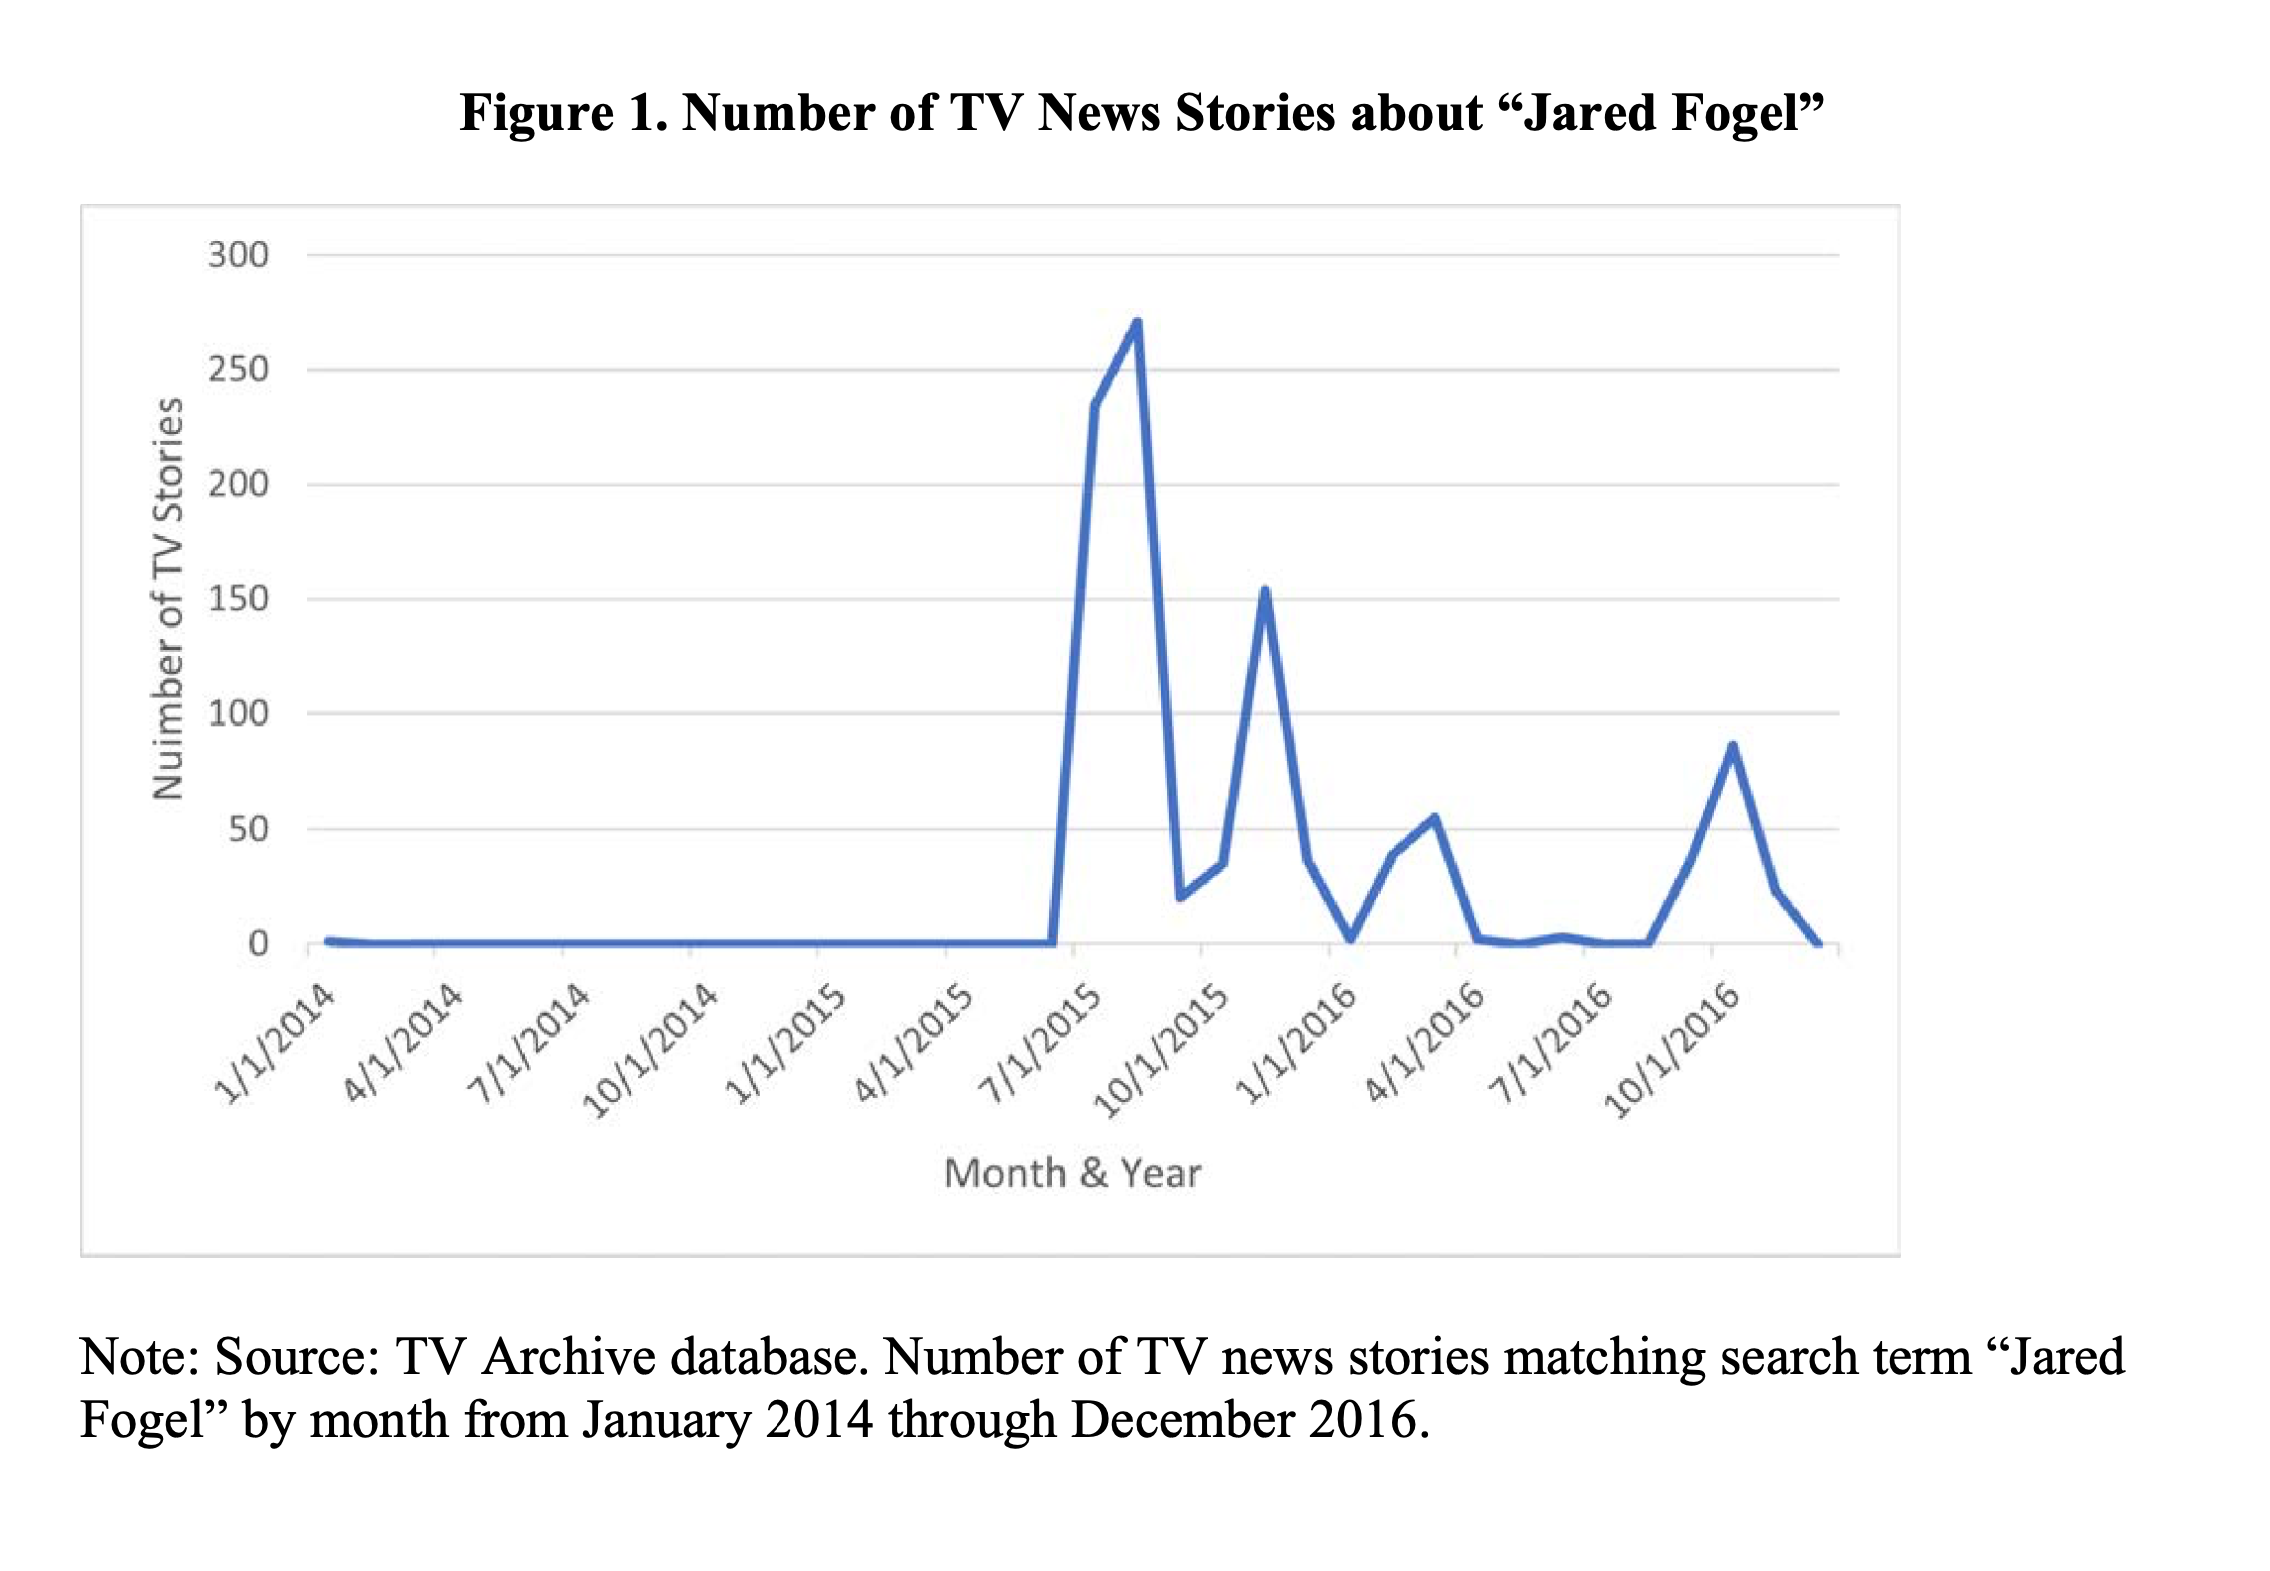
\includegraphics[scale=0.25]{./lecture_includes/subway_1.png}
	\end{figure}

\end{frame}


\begin{frame}{Subway franchise and Scandal}

	\begin{figure}
	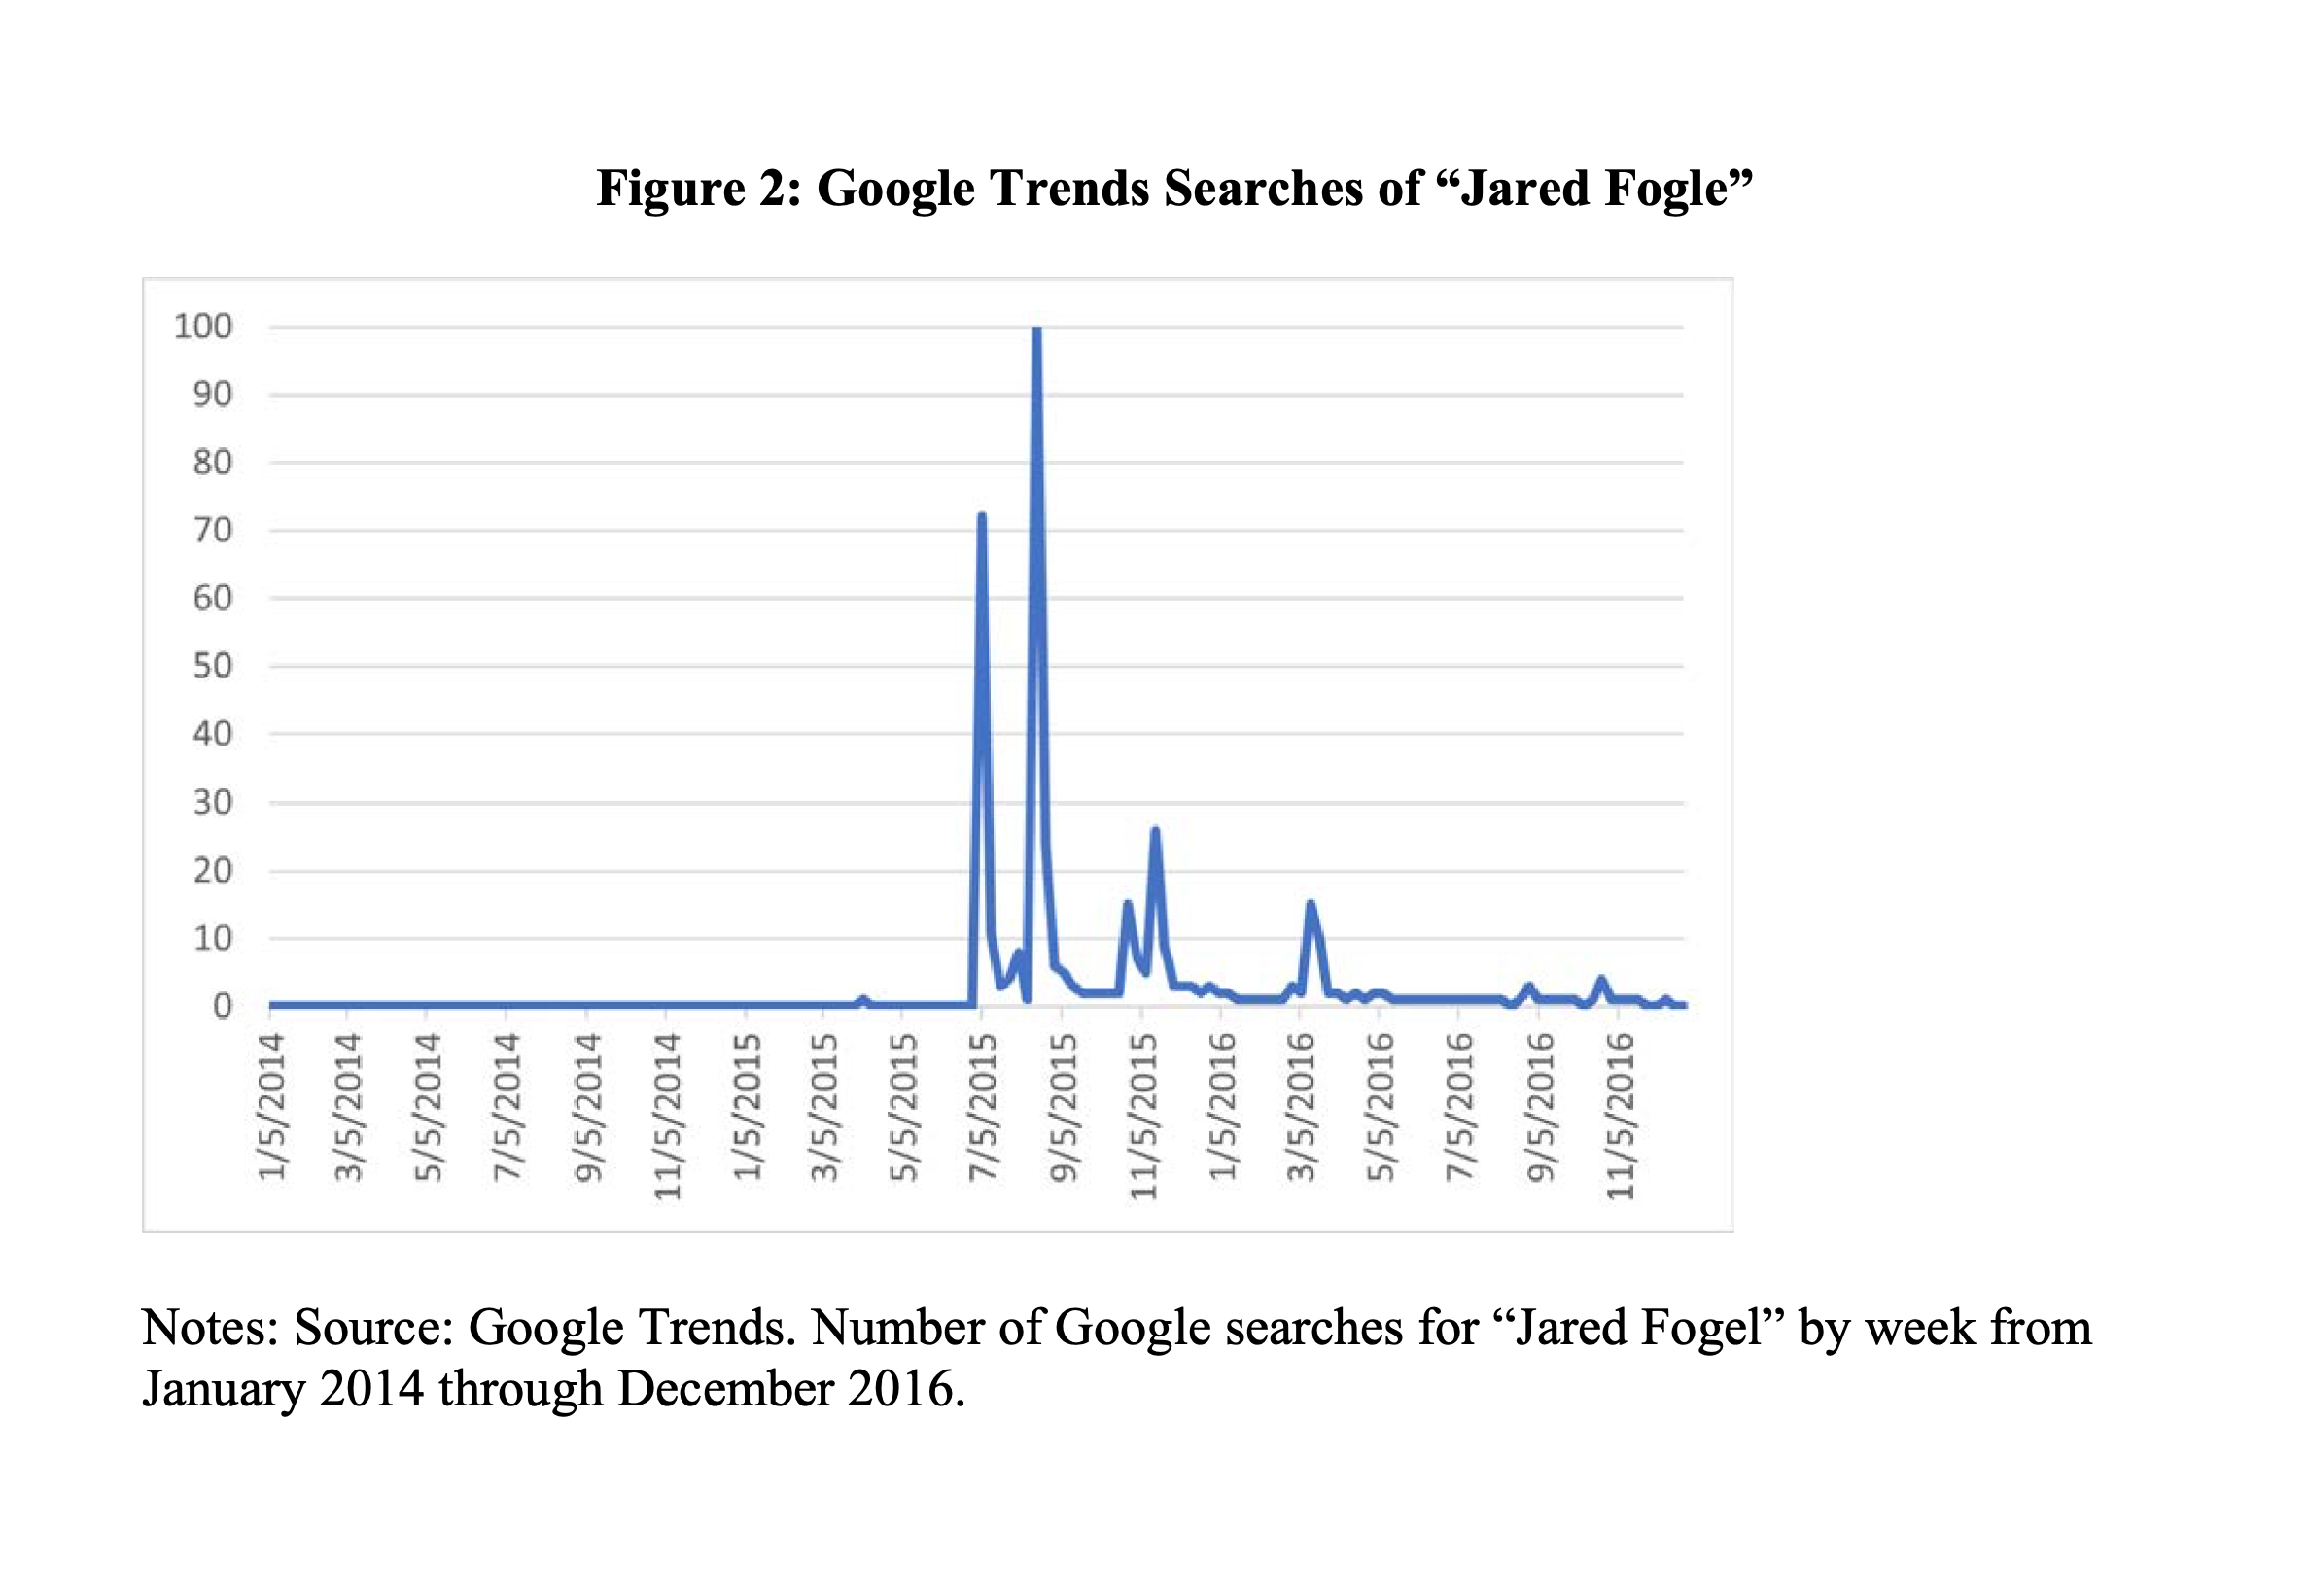
\includegraphics[scale=0.25]{./lecture_includes/subway_2.png}
	\end{figure}

\end{frame}

\begin{frame}{Subway franchise and Scandal}

	\begin{figure}
	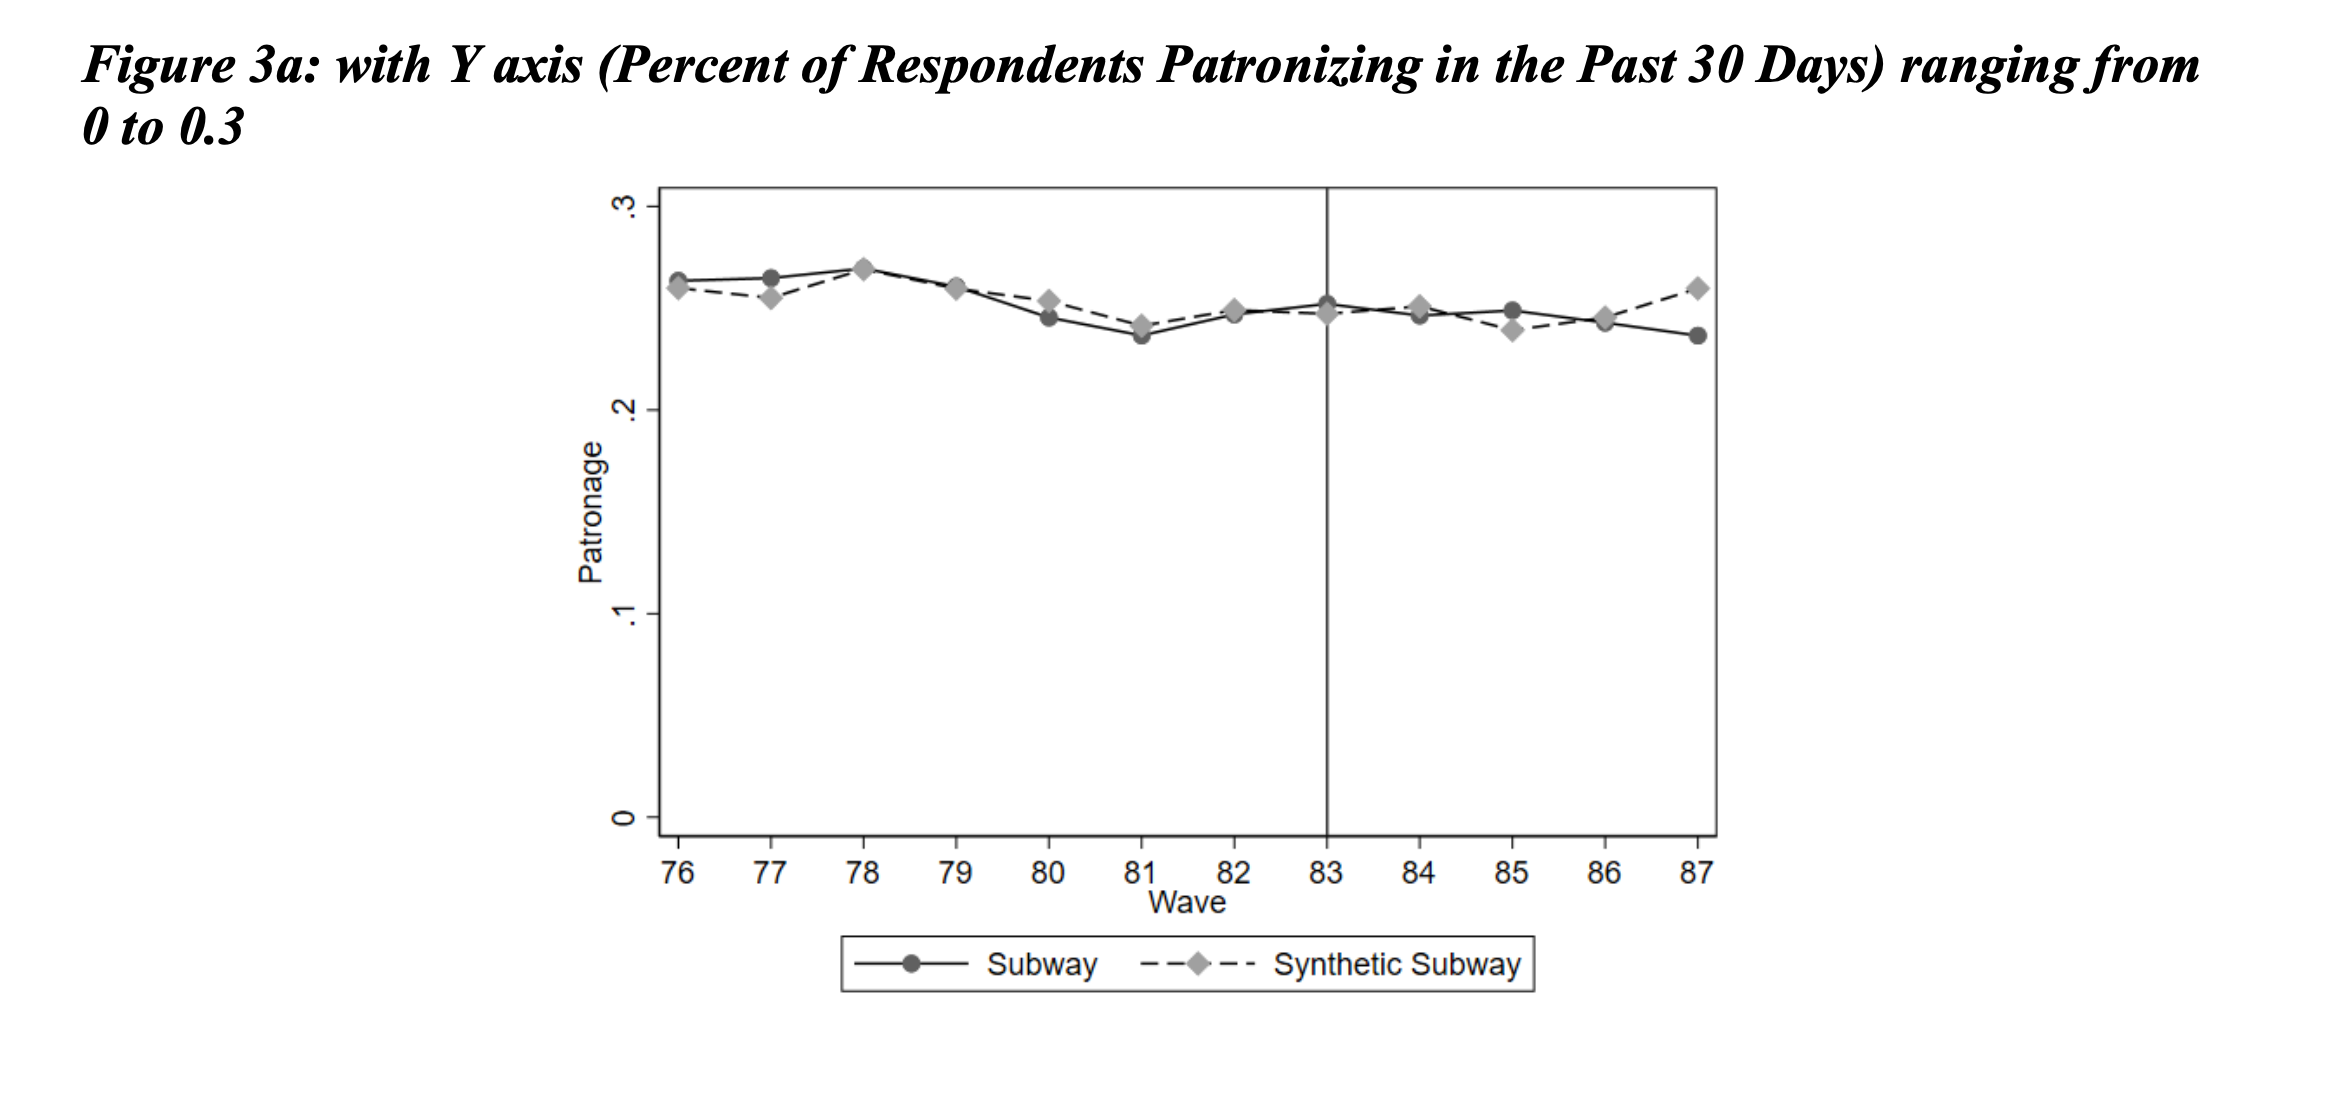
\includegraphics[scale=0.3]{./lecture_includes/subway_3.png}
	\end{figure}

\end{frame}


\begin{frame}{Subway franchise and Scandal}

	\begin{figure}
	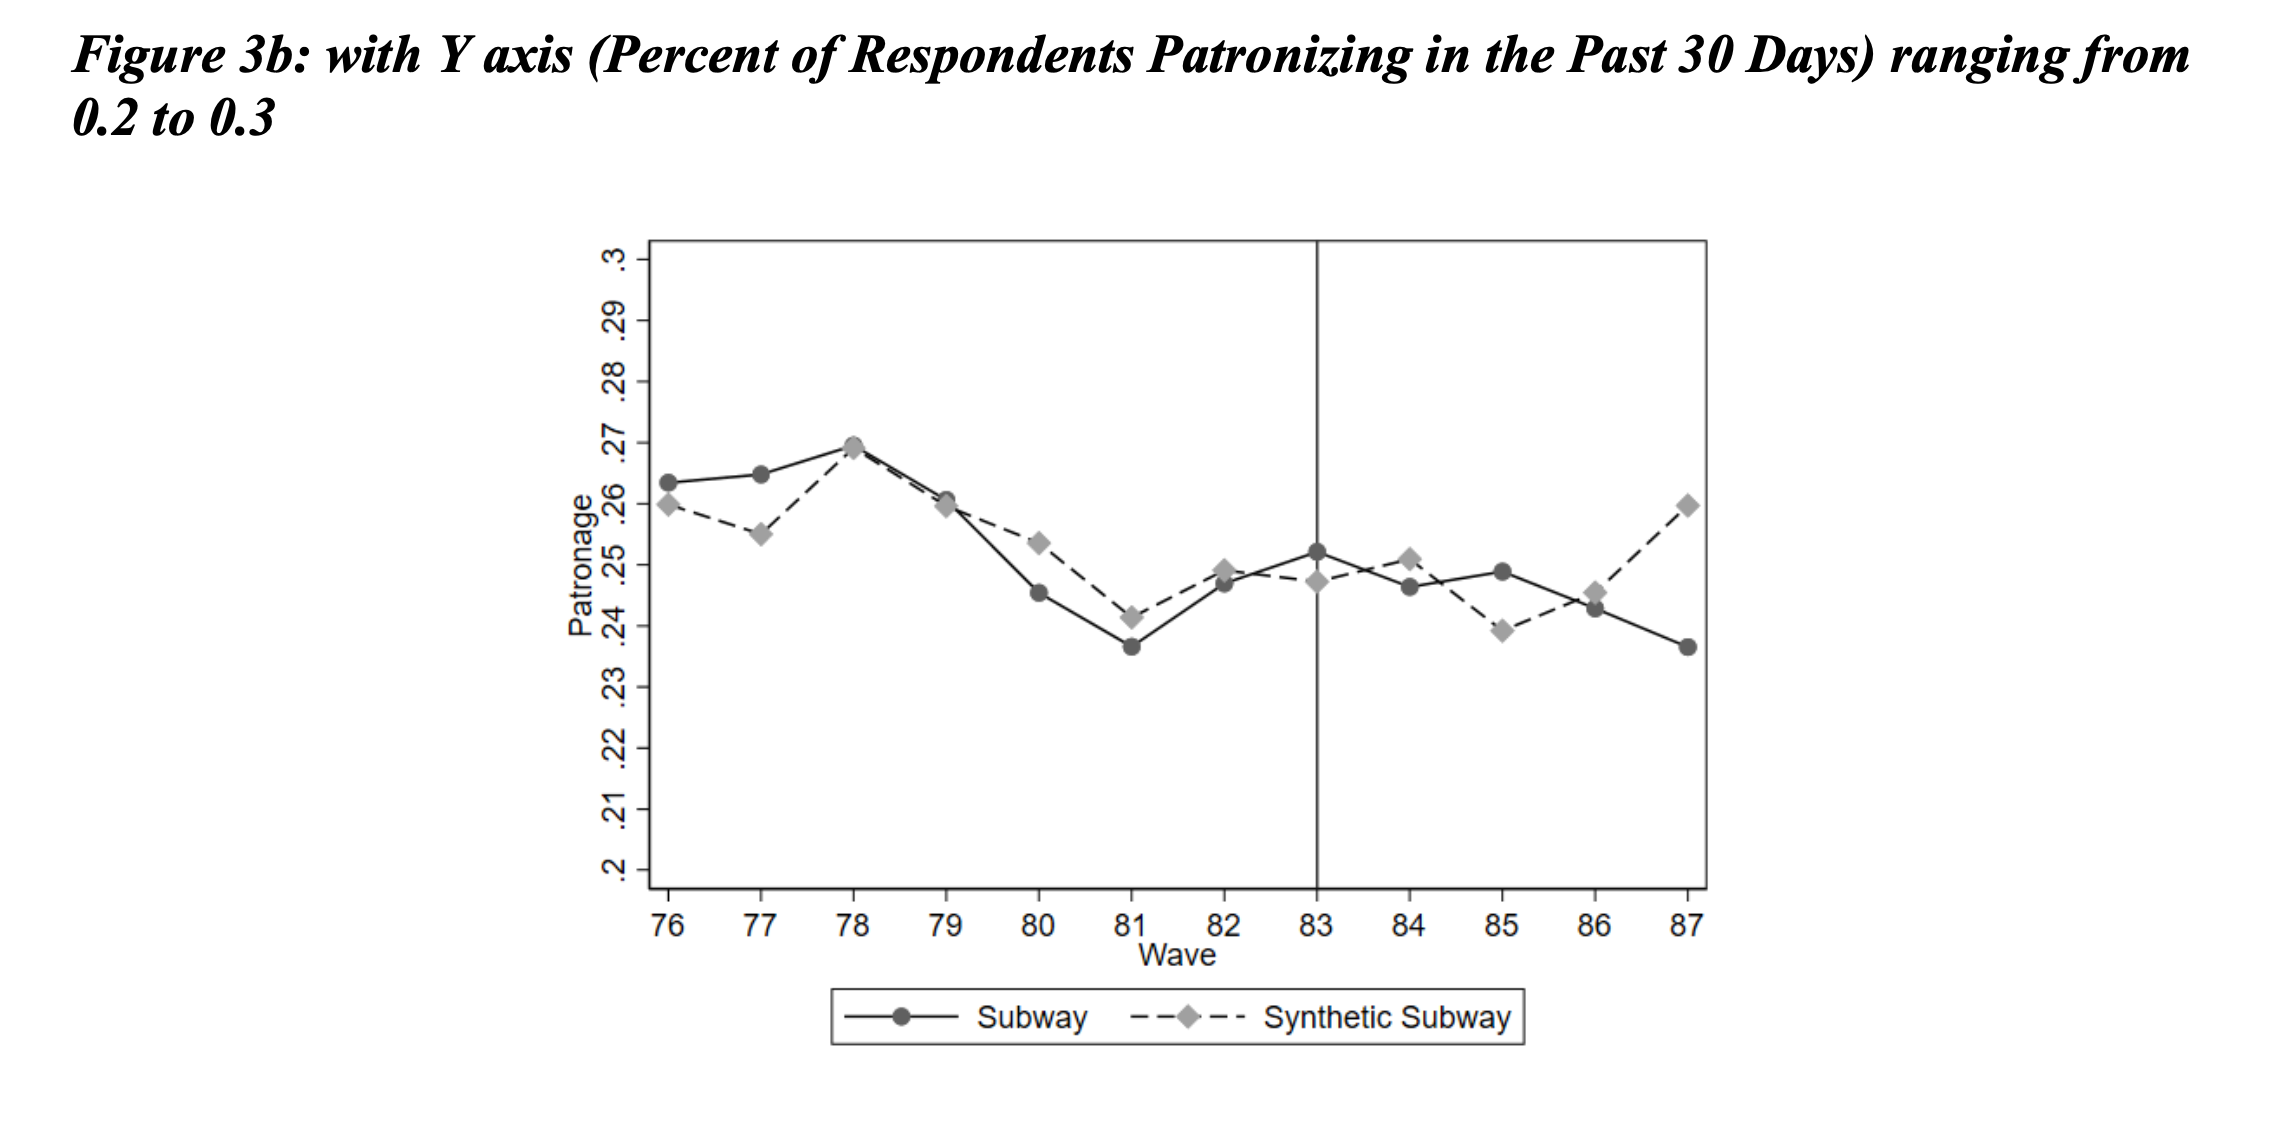
\includegraphics[scale=0.3]{./lecture_includes/subway_4.png}
	\end{figure}

\end{frame}

\begin{frame}{Subway franchise and Scandal}

	\begin{figure}
	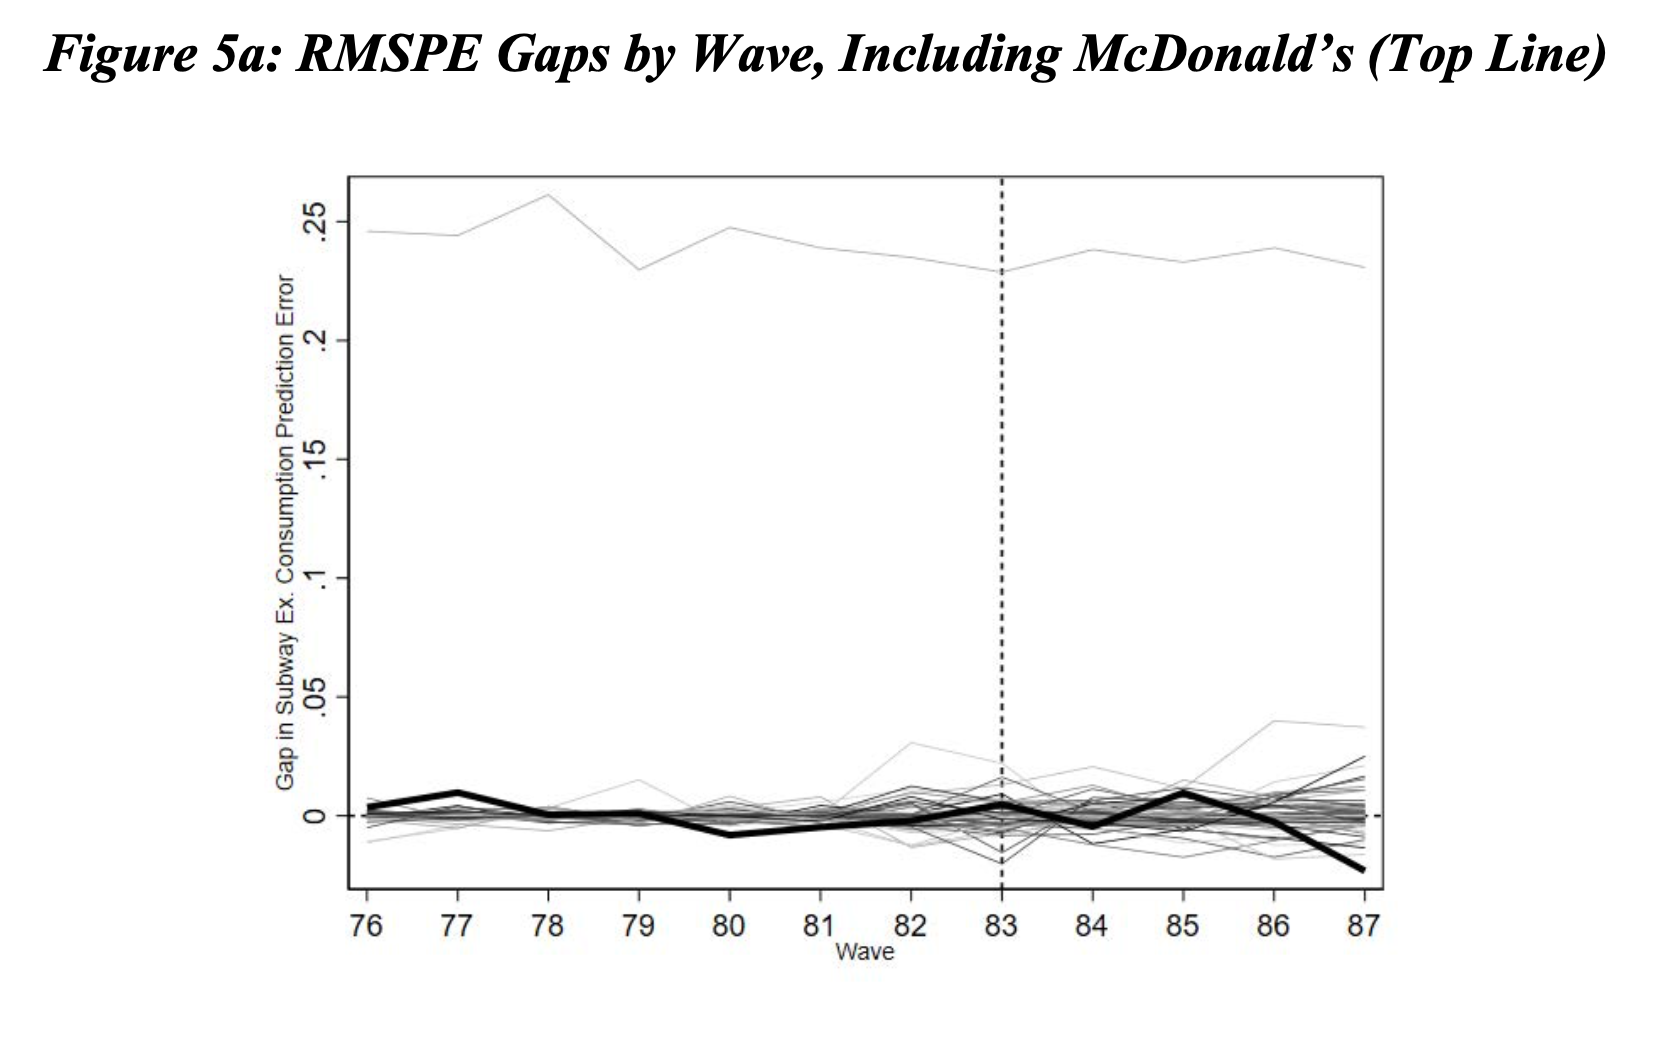
\includegraphics[scale=0.35]{./lecture_includes/subway_5.png}
	\end{figure}

\end{frame}

\begin{frame}{Subway franchise and Scandal}

	\begin{figure}
	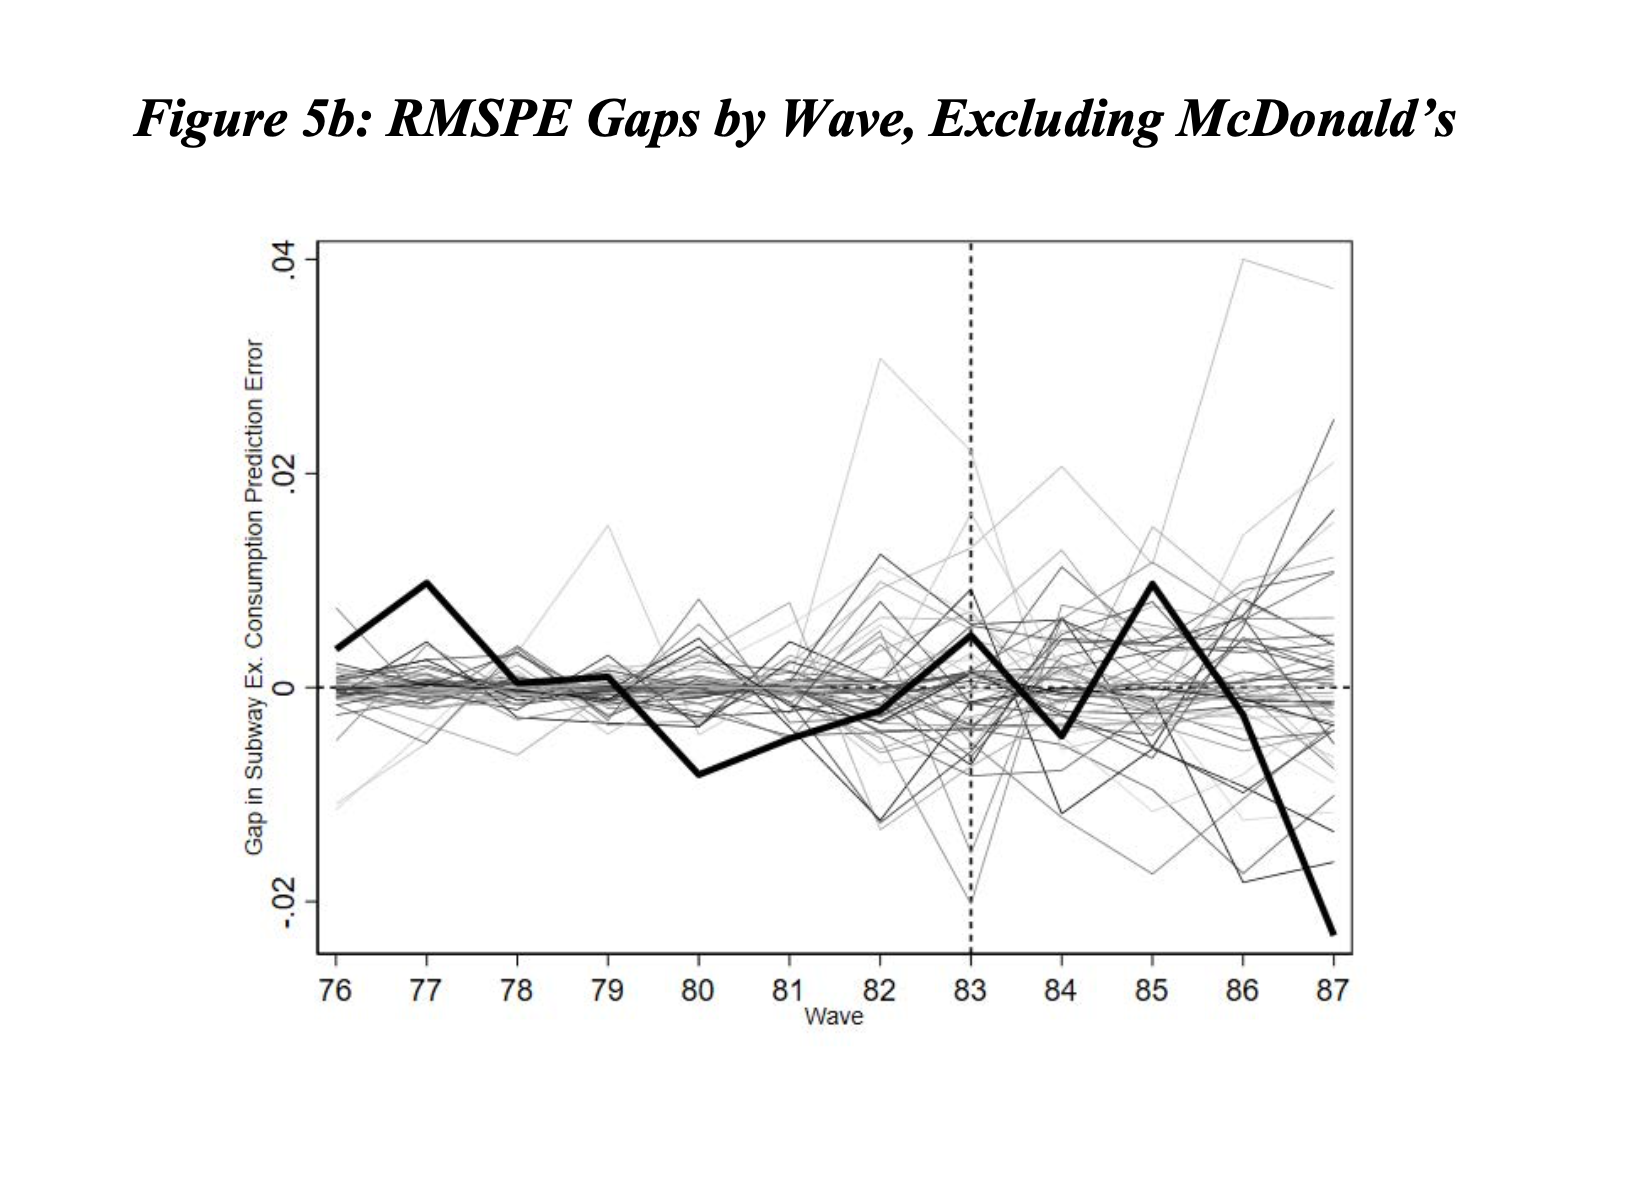
\includegraphics[scale=0.35]{./lecture_includes/subway_6.png}
	\end{figure}

\end{frame}

\begin{frame}{Cherry picking synthetic controls}

\begin{itemize}
\item Abadie, et al. recommended a nested minimization problem using the preintervention data to estimate the SC weights, but very little to no guidance was provided beyond that
\item Historically, a broad range of selection of pre-treatment characteristics were used by early researchers which created researcher degrees of freedom or ``cherry picking synthetic controls''
\item Ferman, Pinto and Possbaum (2020) suggest specific specifications and report all of them with and without covariates
\item Here's an example of the kinds of tables and graphical evidence they suggested researchers follow (followed by what we did)
\end{itemize}

\end{frame}


\begin{frame}{Show p-values across all recommended specifications}

	\begin{figure}
	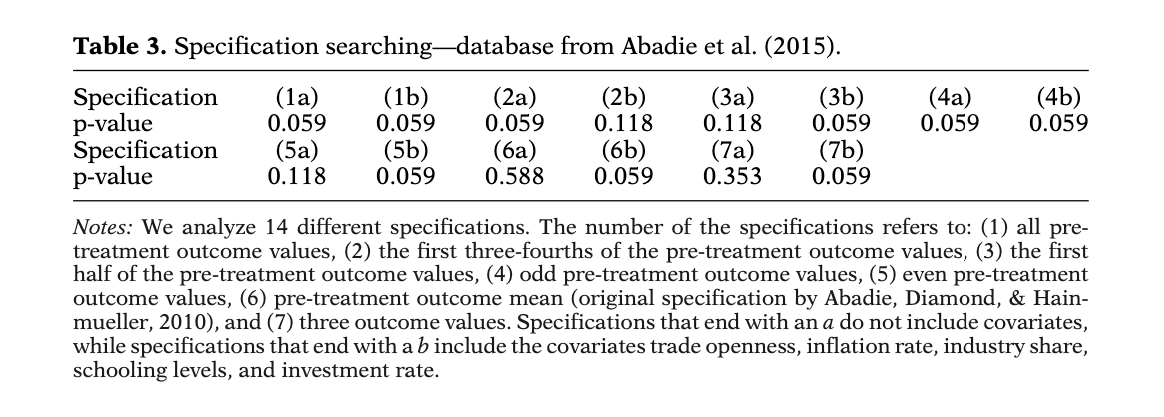
\includegraphics[scale=0.5]{./lecture_includes/cherry_picking_1.png}
	\end{figure}

\end{frame}

\begin{frame}{Show event study (not placebo) across all recommended specifications}

	\begin{figure}
	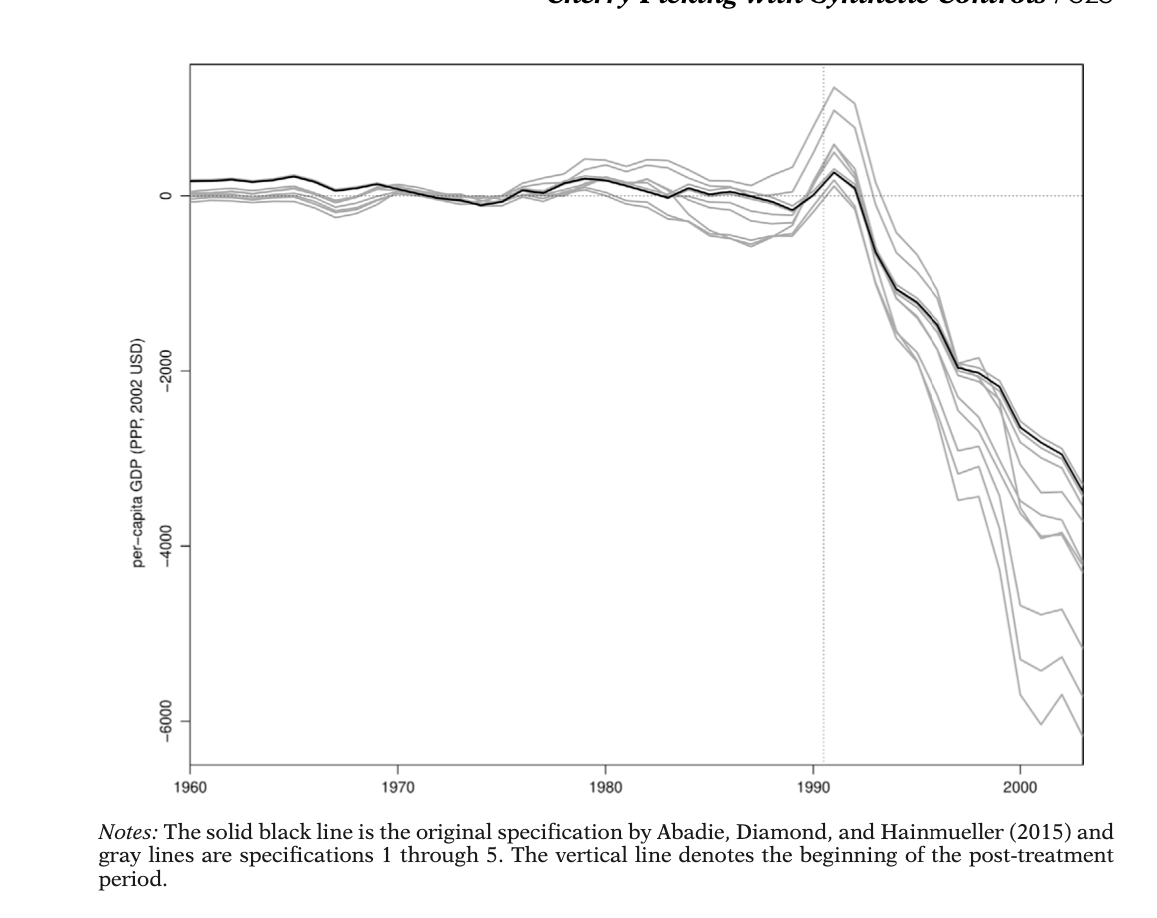
\includegraphics[scale=0.5]{./lecture_includes/cherry_picking_2.png}
	\end{figure}

\end{frame}


\begin{frame}{Subway franchise and Scandal}

	\begin{figure}
	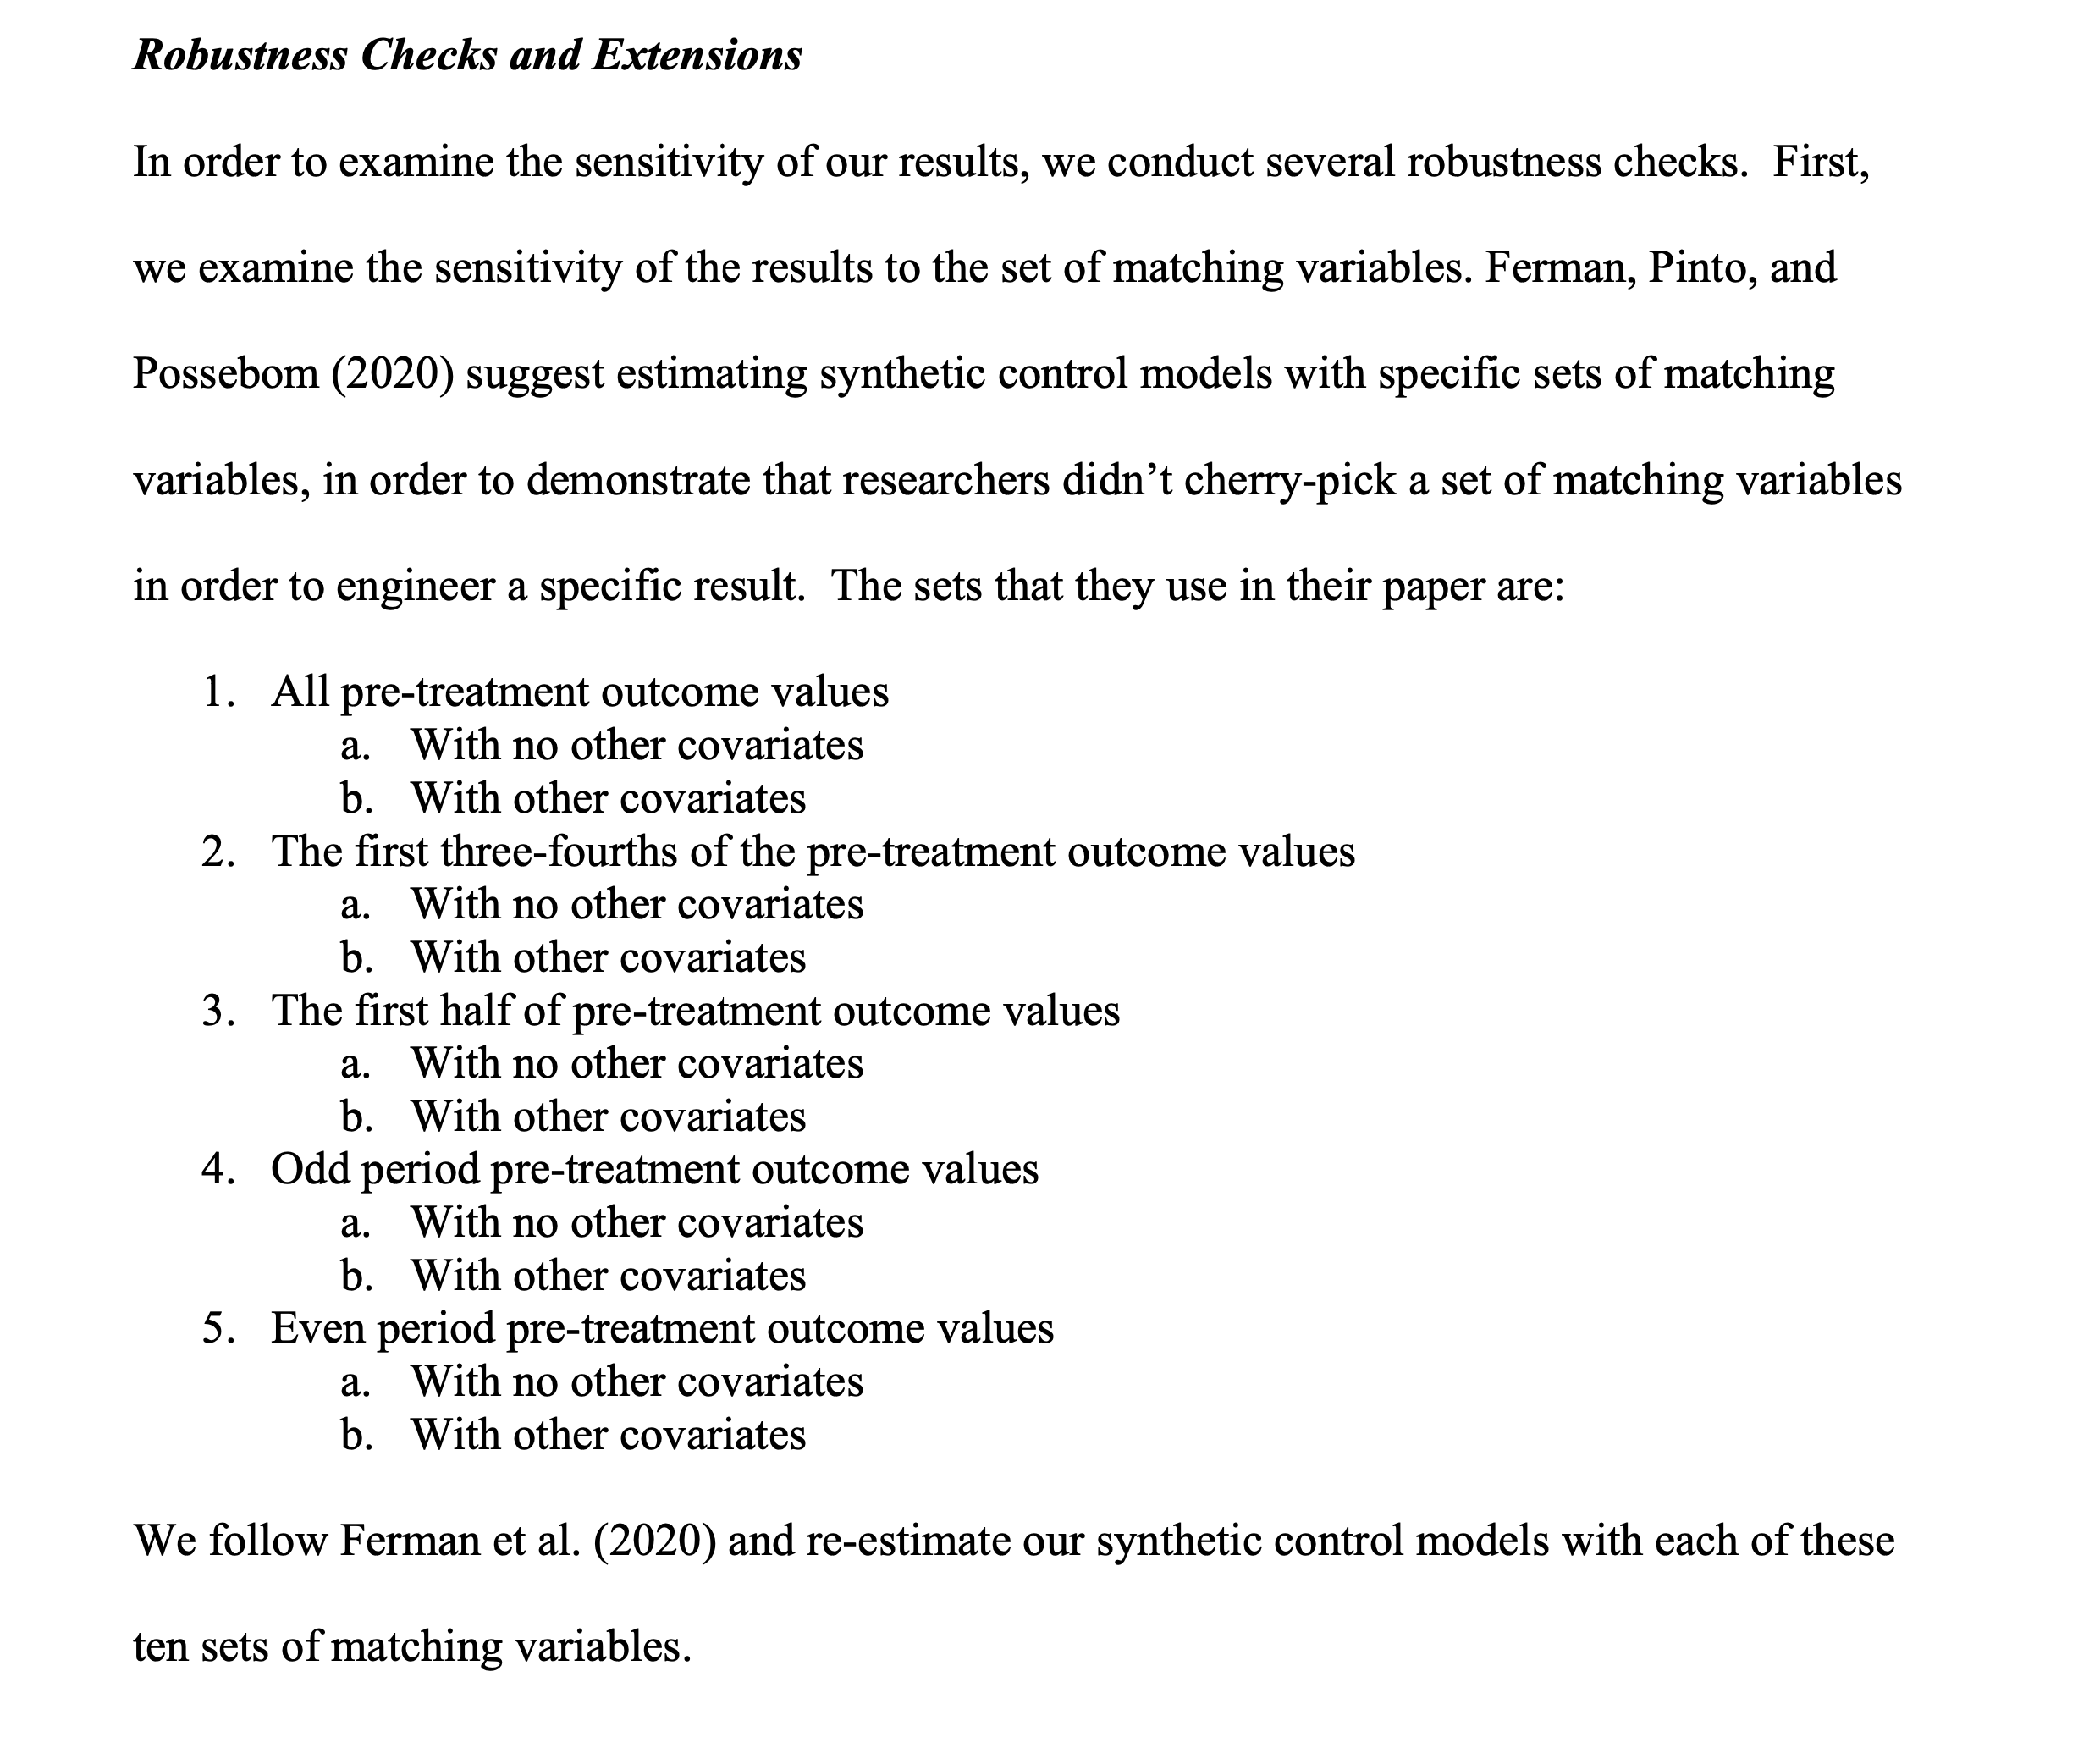
\includegraphics[scale=0.25]{./lecture_includes/subway_robustness.png}
	\end{figure}

\end{frame}


\begin{frame}{Subway franchise and Scandal}

	\begin{figure}
	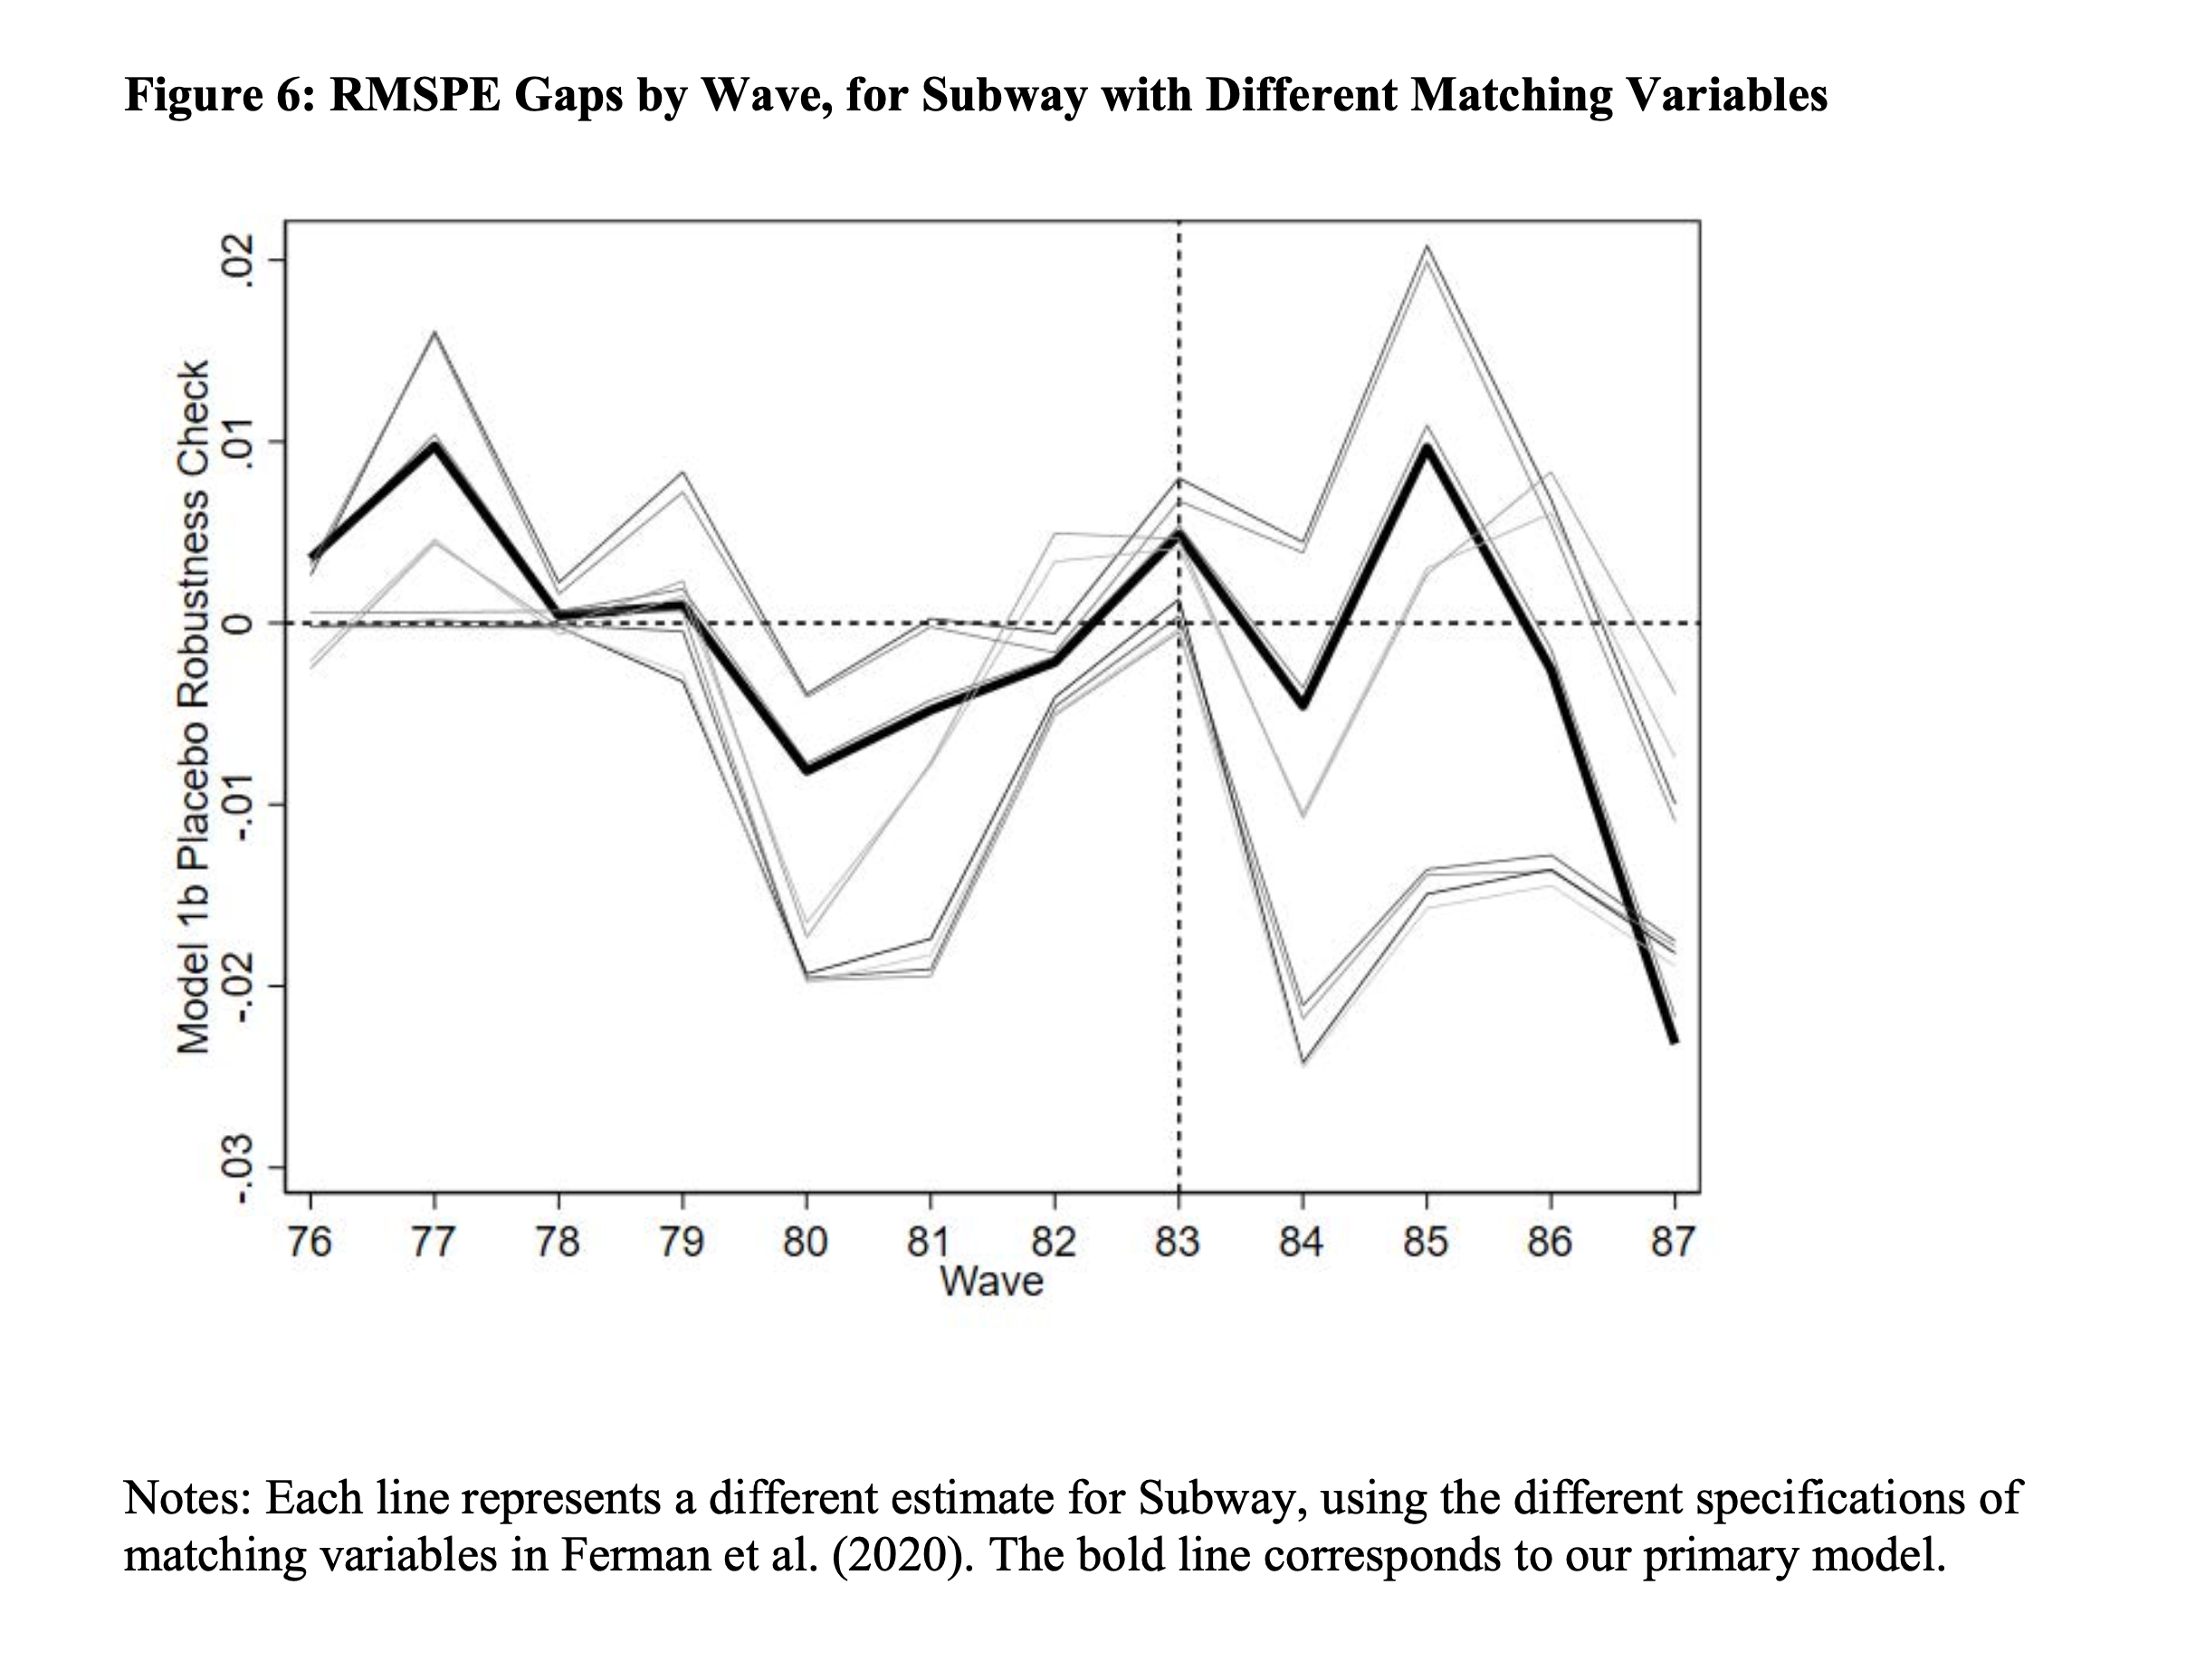
\includegraphics[scale=0.25]{./lecture_includes/subway_7.png}
	\end{figure}

\end{frame}

\begin{frame}{Summarizing}

\begin{itemize}

\item Method is simple: take donor pool units and find a combination of units, weight them, that minimize a distance function subject to two weight constraints $W*$ and $V*$.
\item But what is the bias and what can we do when we think the bias is severe?
\item We now move towards that now by examining the nature of the bias in synthetic control
\end{itemize}

\end{frame}

\begin{frame}{Suppose $Y^0$ is given by a factor model}


\begin{itemize}
\item What about unmeasured factors affecting the outcome variables as well as heterogeneity in the effect of observed and unobserved factors?

\item Abadie, et al. assume that the missing potential outcome, $Y^0_{it}$, is generated using a factor model

\begin{eqnarray*}
Y_{it}^0 = \alpha_t + \theta_t Z_i + \lambda_t u_i + \varepsilon_{it}
\end{eqnarray*}

%where $\alpha_t$ is an unknown common factor with constant factor loadings across units, and $\lambda_t$ is a vector of unobserved common factors

\end{itemize}

\end{frame}

\begin{frame}{Factor Model Intuition}
  Untreated potential outcomes are given by a factor model:
  \begin{equation}\label{eq:untreated_po}
    Y_{it}^0 = \alpha_t + \theta_t Z_i + \textcolor{navy}{\lambda_t} \textcolor{orange}{u_i} + \varepsilon_{it}
  \end{equation}

  \begin{itemize}
 \item $Z_i$ is observed features, $u_i$ is unobserved features, $\varepsilon_{it}$ is unit-level transitory shock
    \item $\lambda_t$ is the set of \textcolor{navy}{factors} (macroeconomic shock) at time $t$.
    \item $u_i$ is unit i's \textcolor{orange}{factor loading} (exposure) to the shocks.
  \end{itemize}

  For example, $\lambda_t$ is a shock to the returns to technological ability and $u_i$ is unobserved ability.
\end{frame}


\begin{frame}{Factor Model Intuition}
  Untreated potential outcomes are given by a factor model:
  \begin{equation}\label{eq:untreated_po}
    Y_{it}^0 = \alpha_t + \theta_t Z_i + \textcolor{navy}{\lambda_t} \textcolor{orange}{u_i} + \varepsilon_{it}
  \end{equation}


Suppose we found $W^*$ such that:

 $$\sum^{J+1}w^*_jY_{jt}=Y_{1t}$$ $$\sum^{J+1}w^*_jZ_{j}=Z_{1}$$ and so on. This may only hold approximately in your sample. If you're able to do that, then you can establish a bound on the bias of the estimator.

\end{frame}


\begin{frame}{Synthetic Control Bias Under Factor Model}

\begin{eqnarray*}
  Y^0_{1t} - \sum^{J+1}_{j=2}w^*_jY_{jt} &=& \sum_{j=2}^{J+1} w_j^* \sum_{s=1}^{T_0} \lambda_t \bigg ( \sum_{n=1}^{T_0} \lambda_n'\lambda_n \bigg )
  ^{-1} \lambda_s'(\varepsilon_{js} - \varepsilon_{1s} ) \\
  && - \sum_{j=2}^{J+1} w_j^* (\varepsilon_{jt} - \varepsilon_{1t})
\end{eqnarray*}

\begin{itemize}
  \item If $\sum_{t=1}^{T_0} \lambda_t' \lambda_t$ is nonsingular, then RHS will be close to zero if number of preintervention periods is ``large''  relative to size of transitory shocks 
  \item Only units that are alike in observables and unobservables should produce similar trajectories of the outcome variable over extended periods of time
\end{itemize}

\end{frame}

\begin{frame}{Synthetic control bounds}

\begin{itemize}
  \item Abadie, et al. 2010 shows the bounds on the bias and it is based on how closely you're able to fit the synthetic control to the treatment group over time
  \item Bias bound is controlled by a ratio between the scale of the transitory shocks, $\varepsilon_{it}$, and the time length
  \item Your credibility of a synthetic control depends on the extent to which it is able to fit a trajectory  $Y_{1t}$ for an extended pre-intervention period
 \end{itemize}
 
 \end{frame}



\begin{frame}{Example of long $T_0$ and transitory shocks}

	\begin{figure}
	
\includegraphics[scale=0.25]{./lecture_includes/restud_titlepage}
	\end{figure}

\end{frame}

\begin{frame}{Example of long $T_0$ and transitory shocks}

	\begin{figure}
	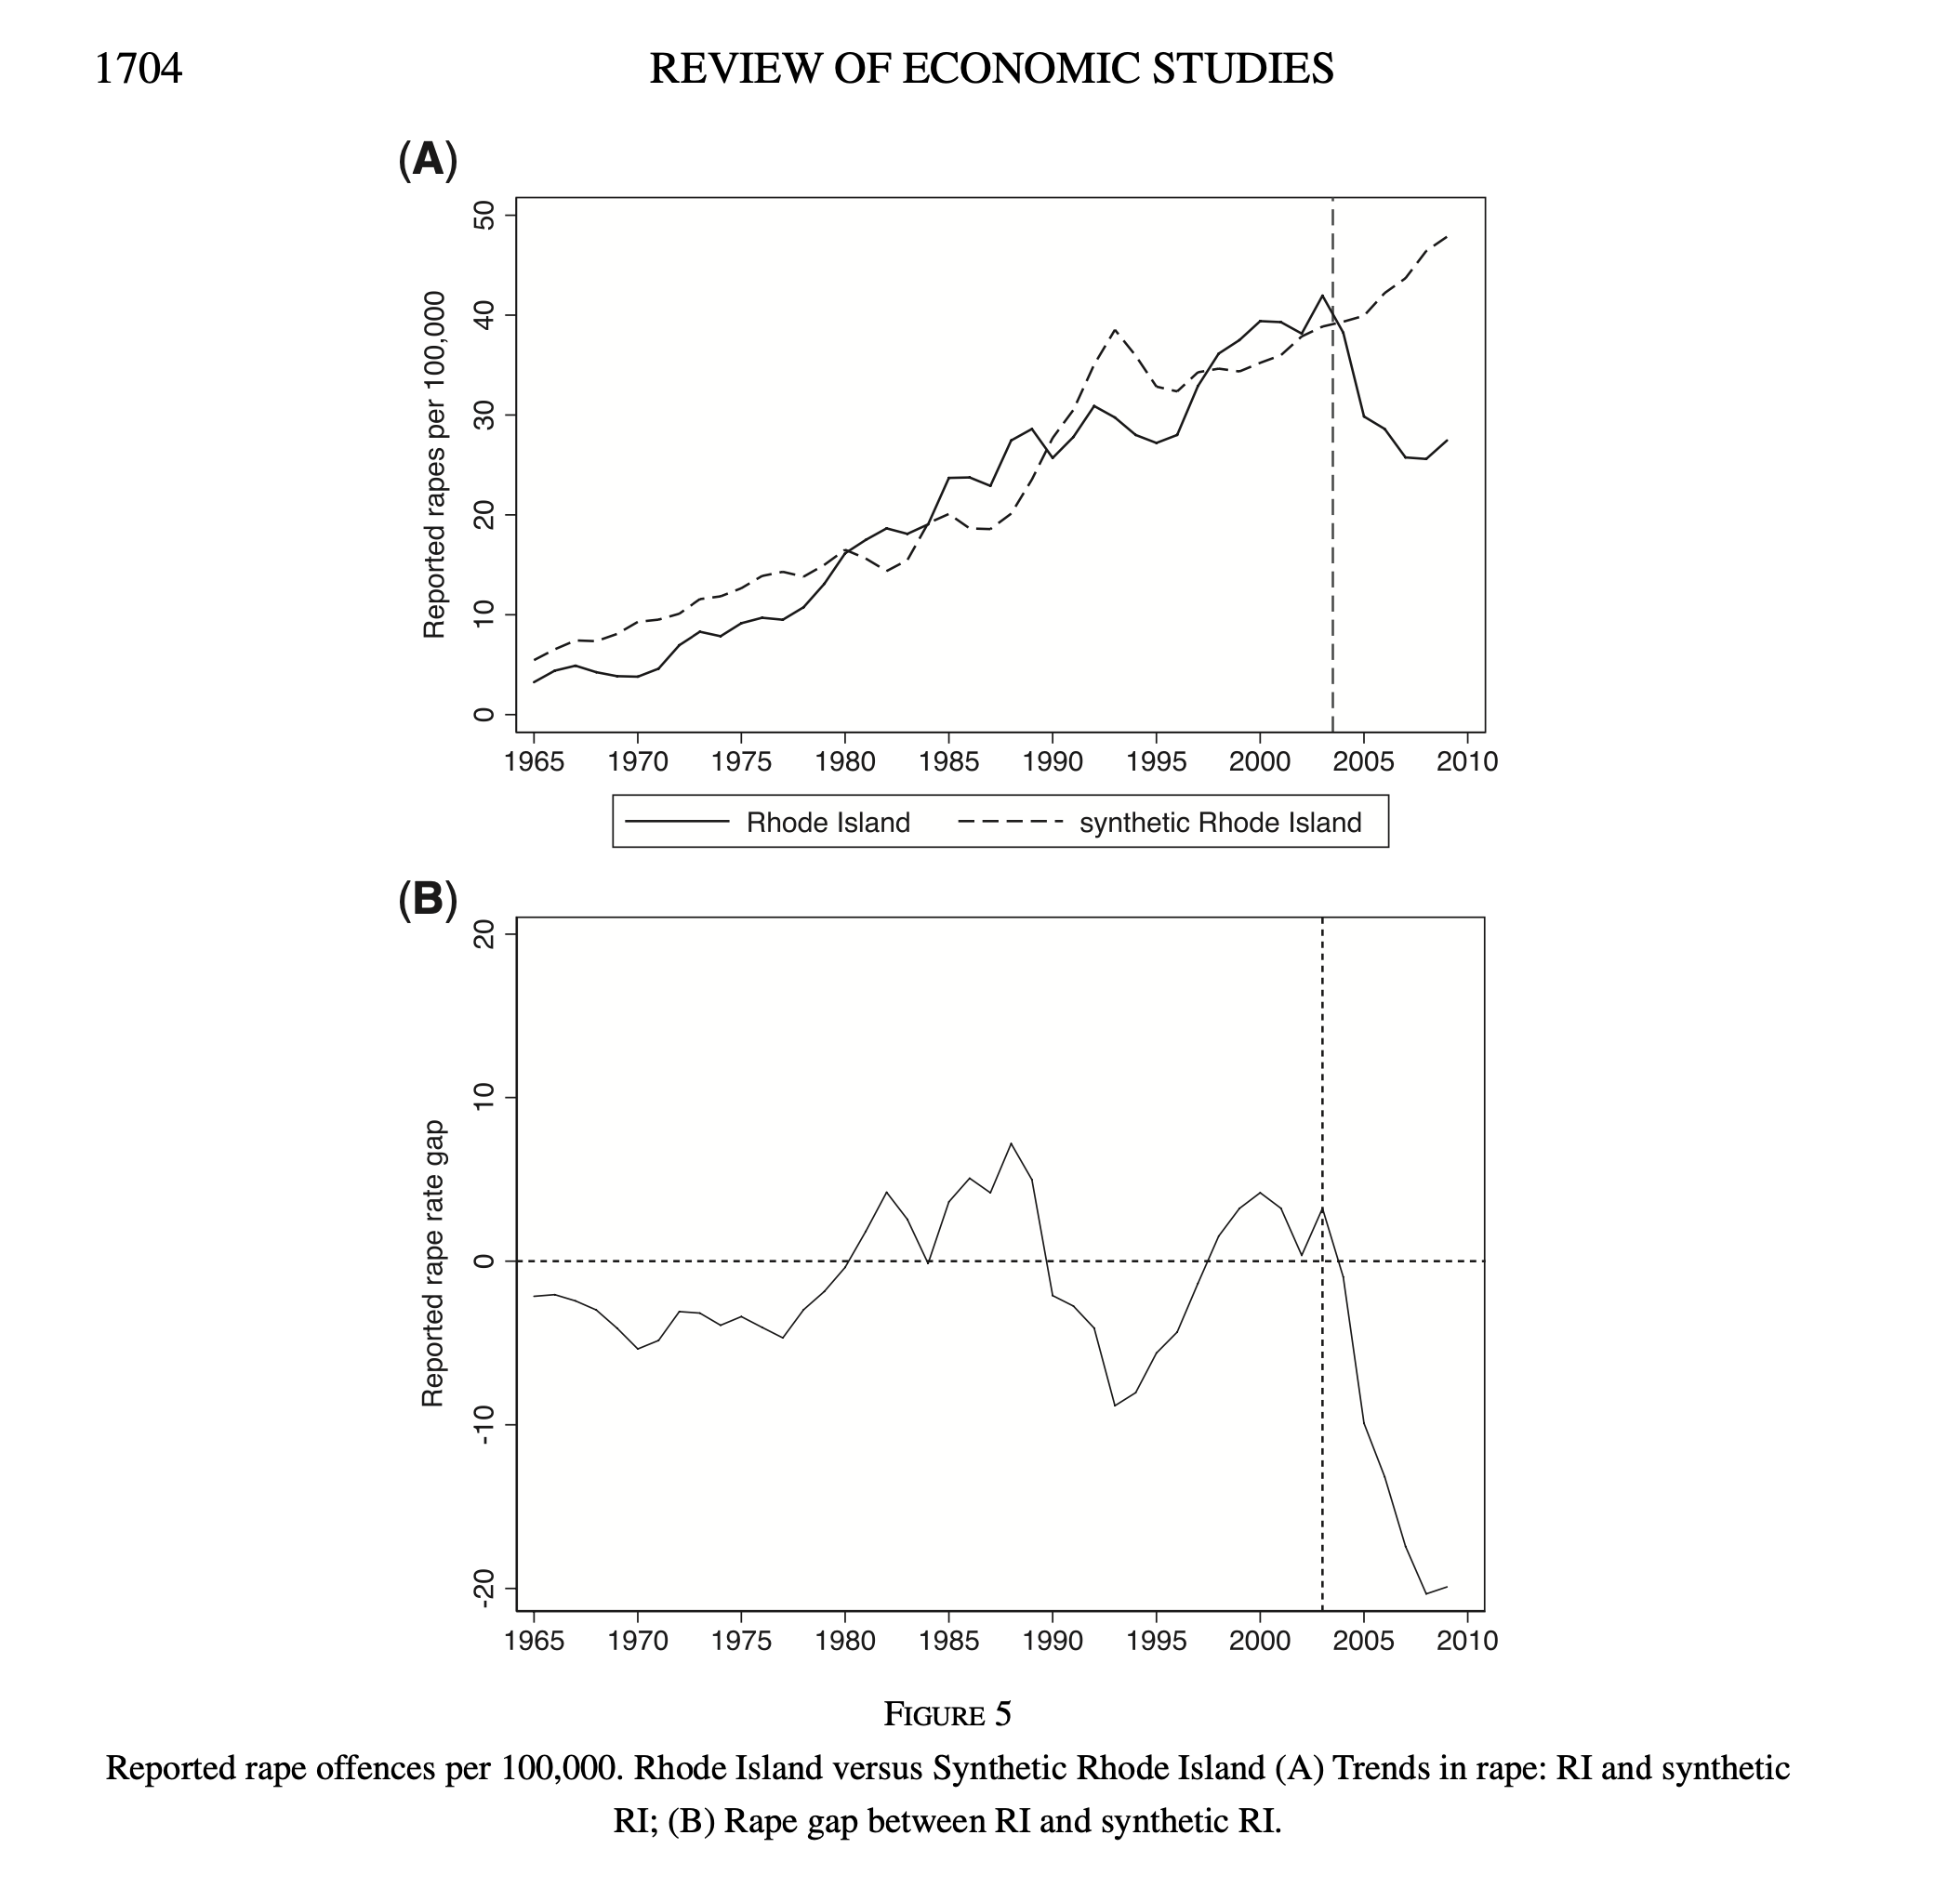
\includegraphics[scale=0.20]{./lecture_includes/restud_rapesynth}
	\end{figure}

\end{frame}




\begin{frame}{ Synthetic Control Bias Under Factor Model}
  Synthetic control will do well when you have many time-periods because:
  \begin{enumerate}
    \item You will not fit on the error term $\varepsilon_{it}$ 
    \item Instead, you will find a synthetic control with the same \emph{exposure} to aggregate shocks (matching on factor-loadings)
  \end{enumerate}

  \bigskip
  But what about when we don't have good fit?
\end{frame}

\subsection{Imperfect fit: Demeaned synthetic control}

\begin{frame}{From Abadie, et al. (2010)}

	\begin{figure}
	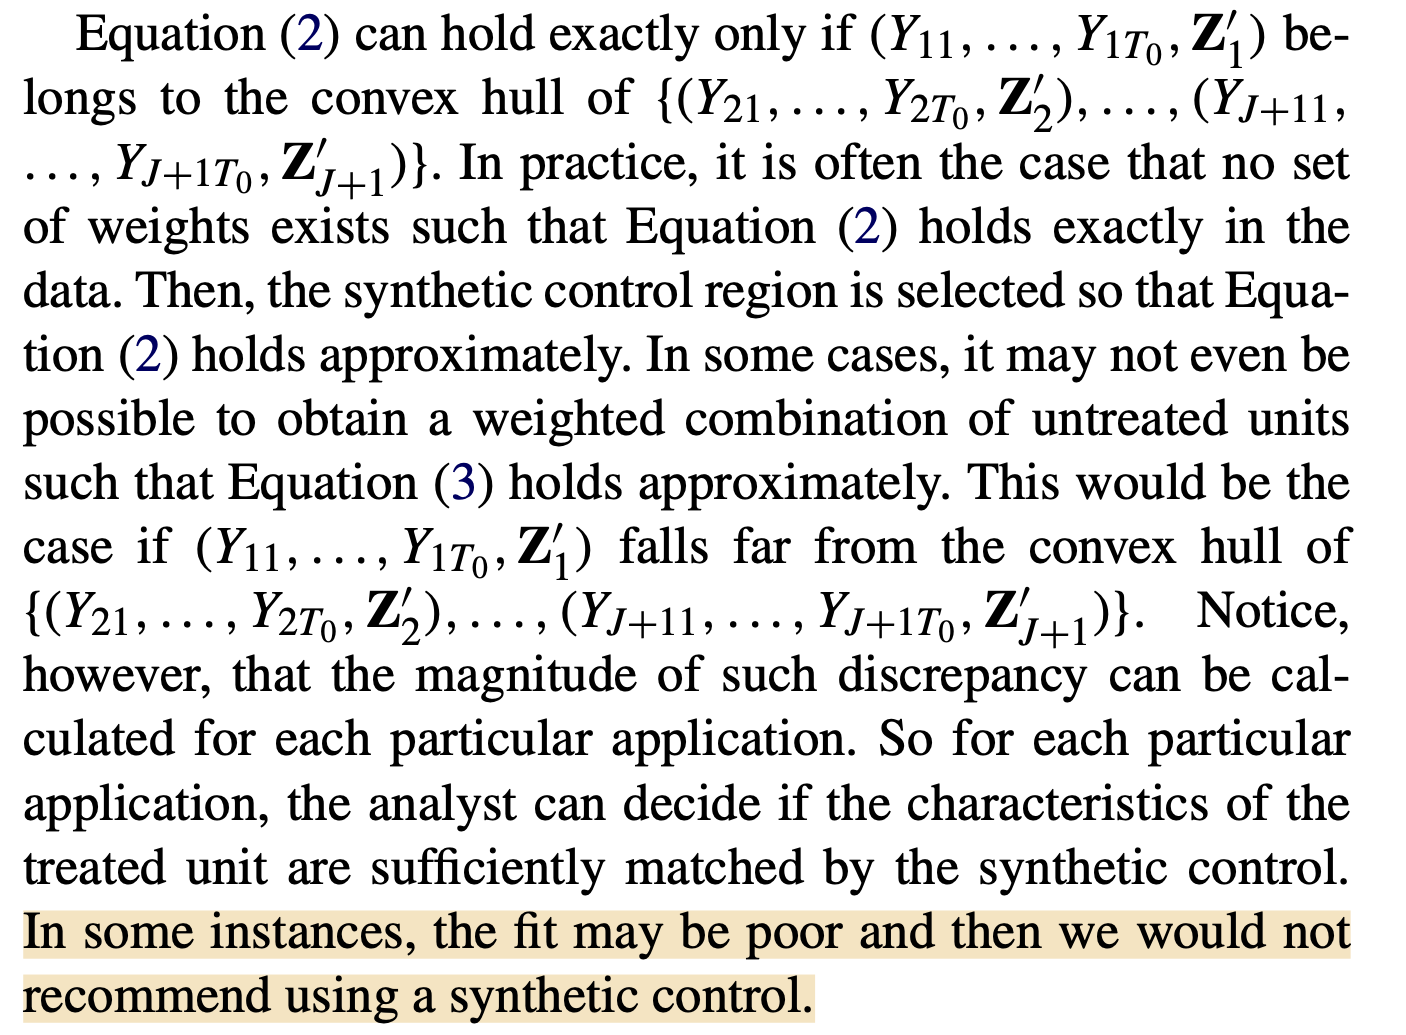
\includegraphics[scale=0.40]{./lecture_includes/abadie_imperfect_fit}
	\end{figure}

\end{frame}


\begin{frame}{Ferman and Pinto (2021)}

	\begin{figure}
	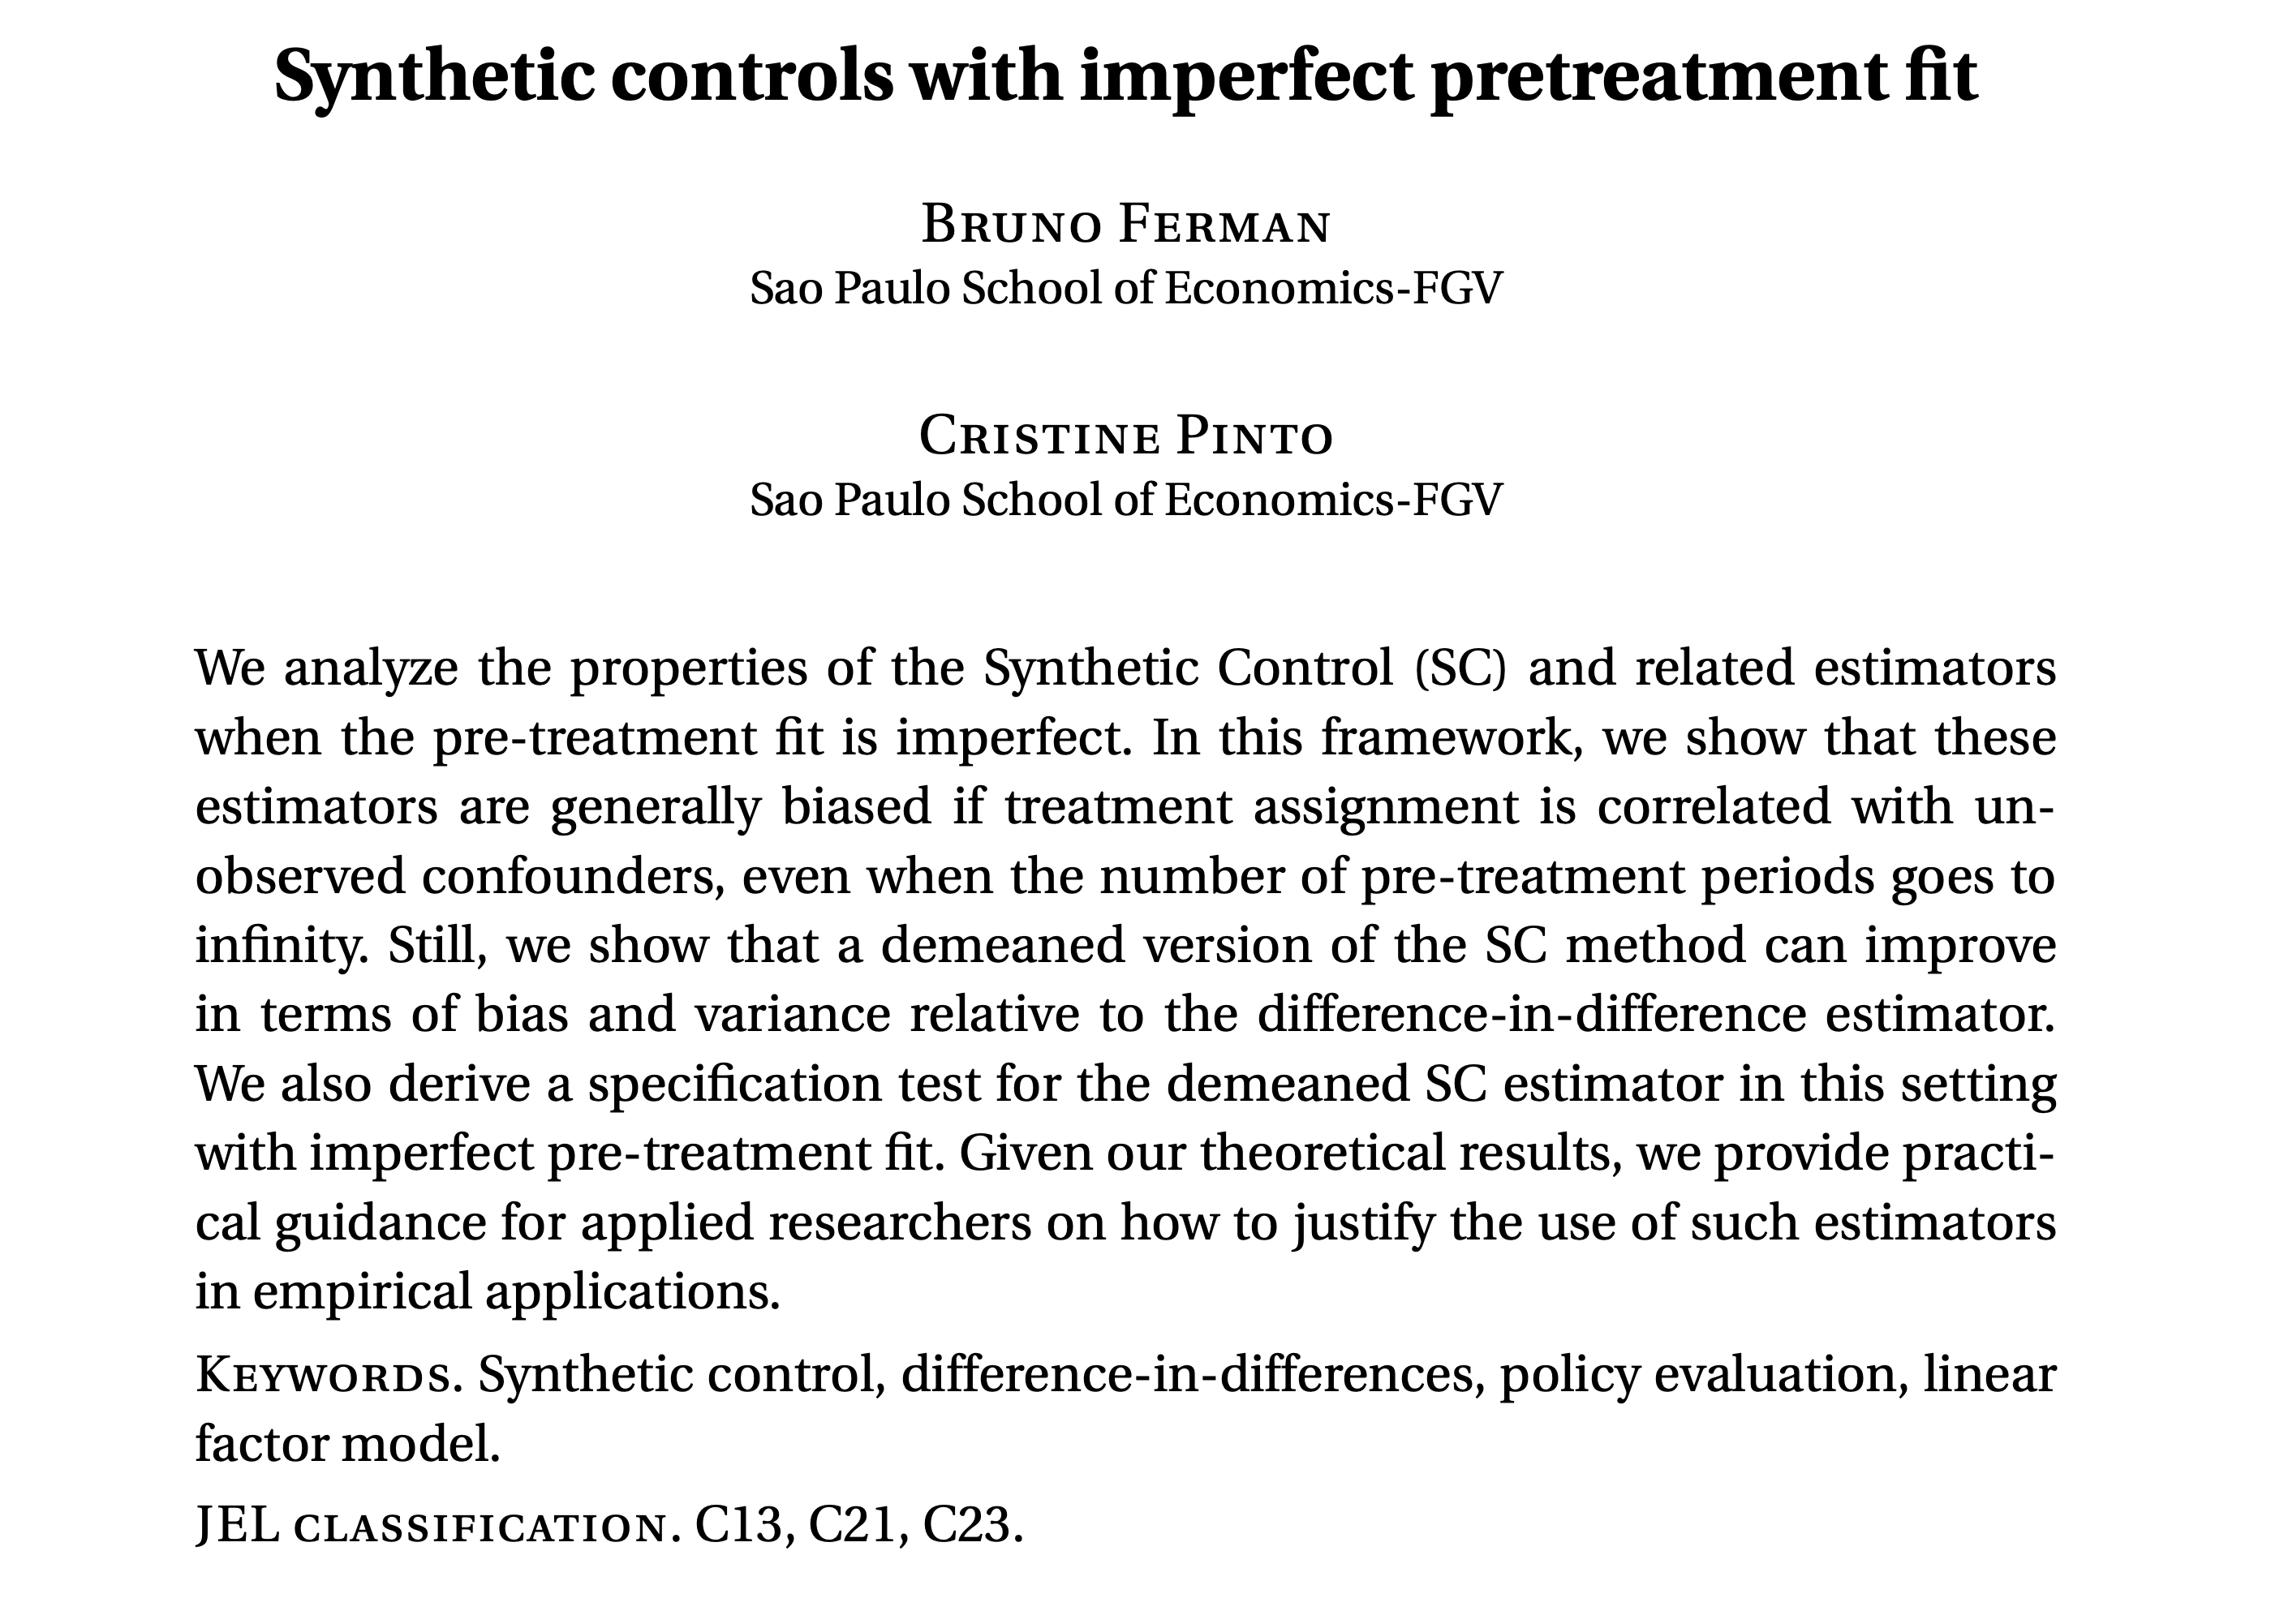
\includegraphics[scale=0.20]{./lecture_includes/ferman_pinto2021}
	\end{figure}

\end{frame}






\begin{frame}{Imperfect pre-treatment fit }

\begin{itemize}

\item Ferman and Pinto (2021) show that synthetic control will generally be biased if treatment assignment is correlated with an unobserved confounder even in very long pre-treatment periods

\item ``This happens because, in this setting, the SC weights converge to weights that simultaneously attempt to match the factor loadings of the treated unit and to minimize the variance of a linear combination of the idiosyncratic shocks.'' (Ferman and Pinto 2021)

\item So even if you reconstructed the pre-trends with your synth, you may not have recovered the true weights because you'd need a comparison group that was affected by the dynamic confounder in exactly the same way, just not treated

\end{itemize}

\end{frame}


\begin{frame}{Demeaning to address bias}

\begin{itemize}
\item Ferman and Pinto (2021) show that the synthetic control estimator converges to the parameter we want \emph{plus linear} combinations of contemporaneous idiosyncratic shocks and common factors
\item If you assume the idiosyncratic factors cancel out in large samples, then the bias will depend on the differences in how the treated and the synthetic control units are affected by the common shocks
\item They show that it is generally unbiased under the same conditions as diff-in-diff, and can have lower asymptotic variance, but they recommend showing then both diff-in-diff and demeaned synthetic control

\end{itemize}

\end{frame}



\begin{frame}{Demeaning to address bias}

\begin{itemize}

\item Cannot compare the original synthetic control with the demeaned synthetic control in terms of bias and variance -- if units with similar factor loadings have similar fixed effects, then matching on levels would be better than demeaning 
\item Demeaning can increase the variance in finite pre-treatment
\item Demeaning also implies extrapolating which is often considered to be one of the hallmark strengths of the original synthetic control estimator -- it does not extrapolate 

\end{itemize}

\end{frame}

\begin{frame}{What did we do?}

\begin{itemize}
\item Our Rhode Island paper began in 2009 and was published in 2018, with working papers in circulation in 2014, well before this imperfect literature
\item One of our main outcomes was reported female rape offenses per 100,000 as measured in the Uniform Crime Reports 
\item Rhode Island is a small state so even relatively modest changes year to year in reported rape offenses caused meaningful swings in the outcome series
\item Our solution was to ``smooth'' using a moving average of each two years -- which was not a demeaning, but rather simply $\frac{Y_t + Y_{t+1}}{2}$
\end{itemize}

\end{frame}





\subsection{Imperfect fit: Augmented Synthetic Control}

\begin{frame}{Augmented Synthetic Control}
\begin{itemize}
\item Synthetic control has built in constraints forcing weights to be non-negative
\item Convex hull constraint ensures that synth is a feasible counterfactual in that it is formed by a combination of control units similar on pre-intervention characteristics
\item Improves the validity of the estimated effect as there exists interpolated comparison group; similar to common support concept
\item But, the convex hull constraint reduces extrapolation bias from comparing dissimilar units, but at the cost of failing to find matches at all
\end{itemize}

\end{frame}



\begin{frame}{What is augmented synthetic control?}

\begin{itemize}
\item Eli Ben-Michael, Avi Feller and Jesse Rothstein present a modification to ADH in which they allow for negative weights, but only minimally so
\item Model will ``augment'' the original synthetic control model by adjusting for pre-treatment imbalance using doubly robust bias adjustment (Abadie and Imbens 2011)
\item Augmentation is conservative negative re-weighting using \textbf{penalized ridge regression} with constraints such that the negative weighting is only to the convex hull, not to the center of the convex hull (does not over-weight)
\end{itemize}

\end{frame}




\begin{frame}{Gist of their argument}

\begin{enumerate}
\item ADH (``synth'') needs perfect fit and so is biased in practical settings due to the curse of dimensionality as it won't be the case we get weights constrained to be ``on the simplex''
\item Their augmentation will introduce an outcome model to estimate the bias caused by covariate imbalance 
\item Introduces ridge regularization linear regression to estimate new weights to reweight synth
\item Think of it as ``bias reduction'' like Abadie and Imbens (2011) plus it will have doubly robust properties and be equivalent to inverse probability weighting
\item When synth is imbalanced, augmented synth will reduce bias reweighting and bias correction, and when synth is balanced, they are the same
\end{enumerate}

\end{frame}


\begin{frame}{Gist of their argument}

\begin{enumerate}
\item Ridge regularization linear regression used to estimate weights used to reweight the original synth model
\item If synth is imbalanced, augmented synth reducees bias by reweighting and bias correction
\item When synth is balanced, the augmented and original synth are identical (but in practice, they won't be identical)
\item They argue synth DiD can be seen as a special case of augmented synth
\end{enumerate}

\end{frame}


\begin{frame}{Some topical observations}

\begin{itemize}
\item Foregoes estimating \emph{donor pool unit weights} (e.g., ADH, synth did, MCNN)
\item Synth sequels are using penalization/regularization for estimation
\item Relaxes some of the original ADH constraints, like non-negative weights (i.e., no extrapolation)
	\begin{itemize}
	\item This is used to address bias caused by imbalance
	\item Negative weights puts them back in the convex hull which recall we need
	\item They argue synth DiD can be seen as a special case of augmented synth
	\end{itemize}
\end{itemize}

\end{frame}



\begin{frame}{Notation}

\begin{itemize}
\item Observe $J+1$ units over $T$ time periods
\item Unit $1$ will be treated at time period $T_0=T-1$ (we allow for unit $1$ to be an average over treated units)
\item Units $j=2 $ to $J+1$ (using ADH original notation) are ``never treated''
\item $D_j$ is the treatment indicator
\end{itemize}

\end{frame}


\begin{frame}[plain,shrink=20]
\begin{center}
\textbf{Pre-treatment outcomes}
\end{center}

\begin{center}
\[ \left( \begin{array}{ccccc}
    Y_{11} & Y_{12} & Y_{13} & \dots  & Y_{1T}^1 \\
    Y_{21} & Y_{22} & Y_{23} & \dots  & Y_{2T}^0  \\
    \vdots & \vdots & \vdots & \ddots & \vdots \\
    Y_{N1} & Y_{i2} & Y_{i3} & \dots  & Y_{NT}^0
\end{array} \right) \equiv
\left( \begin{array}{ccccc}
    X_{11} & X_{12} & X_{13} & \dots  & Y_{1} \\
    X_{21} & X_{22} & X_{23} & \dots  & Y_{2}  \\
    \vdots & \vdots & \vdots & \ddots & \vdots \\
    X_{N1} & X_{i2} & X_{i3} & \dots  & Y_{N}
\end{array} \right) \equiv
\left( \begin{array}{cc}
    X_{1} & Y_{1} \\
    X_{0} & Y_{0}  \\
\end{array} \right)
\]

\end{center}

This is a model of 2x2 (i.e., single last period block structure, not staggered roll out)

\bigskip

The last column is always post-treatment and switches from $Y^1$ to $Y$. 

\bigskip

The last column is just showing a top row of the treated unit 1 and the bottom row of all the donor pool (i.e., we will use $X_0$ and $Y_0$ to represent all the donor pool units)

\end{frame}


\begin{frame}{Optimal weights}

Synth minimizes the following norm:

\begin{eqnarray*}
\textrm{min}_w = || V_X^{1/2} (X_1 - X_0'w) ||_2^2 + \psi \sum_{D_j=0}f(w_j)\\
\textrm{s.t. }\sum_{j=2}^N w_{j} =1 \textrm{ and } w_j \geq 0
\end{eqnarray*}

$Y_0'w*$ (i.e., optimally weighted donor pool) is the unit 1 ``synthetic control'' 

\end{frame}


\begin{frame}{Predicting counterfactuals}

Synth minimizes the following norm:

\begin{eqnarray*}
\textrm{min}_w = || V_X^{1/2} (X_1 - X_0'w) ||_2^2 + \psi \sum_{D_j=0}f(w_j)\\
\textrm{s.t. }\sum_{j=2}^N w_{j} =1 \textrm{ and } w_j \geq 0
\end{eqnarray*}

We are hoping that $\widehat{Y}_1^0$ with $Y_0' {w}^{*}$ based on ``perfect fit'' pre-treatment

\end{frame}




\begin{frame}{$V_X$ matrix}

Synth minimizes the following norm:

\begin{eqnarray*}
\textrm{min}_w = || V_X^{1/2} (X_1 - X_0'w) ||_2^2 + \psi \sum_{D_j=0}f(w_j)\\
\textrm{s.t. }\sum_{j=2}^N w_{j} =1 \textrm{ and } w_j \geq 0
\end{eqnarray*}

$V_x$ is the ``importance'' matrix on $X_0$ (Stata default chooses $V_x$ that min pre-treatment MSE).
\end{frame}

\begin{frame}{Penalizing the weights with ridge}

Synth minimizes the following norm:

\begin{eqnarray*}
\textrm{min}_w = || V_X^{1/2} (X_1 - X_0'w) ||_2^2 + \psi \sum_{D_j=0}f(w_j)\\
\textrm{s.t. }\sum_{j=2}^N w_{j} =1 \textrm{ and } w_j \geq 0
\end{eqnarray*}

Modification to the original synthetic control model is the inclusion of the penalty term. ``The choice of penalty is less central when weights are constrained to be on the simplex, but becomes more important when we relax this constrain.''

\end{frame}

\begin{frame}{Convex hull}

Synth minimizes the following norm:

\begin{eqnarray*}
\textrm{min}_w = || V_X^{1/2} (X_1 - X_0'w) ||_2^2 + \psi \sum_{D_j=0}f(w_j)\\
\textrm{s.t. }\sum_{j=2}^N w_{j} =1 \textrm{ and } w_j \geq 0
\end{eqnarray*}

These weights will be used to address imbalance, not so much the control units, bc this method is for when the weighted controls are still outside the convex hull (``simplex'')

\end{frame}




\begin{frame}{Original ADH factor model and bias}

\begin{eqnarray*}
Y_{it}^0 = \alpha_t + \theta_t Z_i + \lambda_t u_i + \varepsilon_{it}
\end{eqnarray*}

\bigskip

Original synth factor model (with ADH notation)

\bigskip

\begin{eqnarray*}
Y^0_{1t} - \sum^{J+1}_{j=2}w^*_jY_{jt} &=& \sum_{j=2}^{J+1} w_j^* \sum_{s=1}^{T_0} \lambda_t \bigg ( \sum_{n=1}^{T_0} \lambda_n'\lambda_n \bigg )
^{-1} \lambda_s'(\varepsilon_{js} - \varepsilon_{1s} ) \\
&& - \sum_{j=2}^{J+1} w_j^* (\varepsilon_{jt} - \varepsilon_{1t})
\end{eqnarray*}

\bigskip

The bias of ADH synthetic control


\end{frame}




\begin{frame}{Perfect fit is necessary}

\begin{eqnarray*}
Y^0_{1t} - \sum^{J+1}_{j=2}w^*_jY_{jt} &=& \sum_{j=2}^{J+1} w_j^* \sum_{s=1}^{T_0} \lambda_t \bigg ( \sum_{n=1}^{T_0} \lambda_n'\lambda_n \bigg )
^{-1} \lambda_s'(\varepsilon_{js} - \varepsilon_{1s} ) \\
&& - \sum_{j=2}^{J+1} w_j^* (\varepsilon_{jt} - \varepsilon_{1t})
\end{eqnarray*}

\bigskip

Recall that the bias of ADH required ``perfect fit'' using their factor model (I'll change $\lambda$ factor loadings in a minute)

\end{frame}




\begin{frame}{Perfect fit models heterogeneity}


\begin{eqnarray*}
Y^0_{1t} - \sum^{J+1}_{j=2}w^*_jY_{jt} &=& \sum_{j=2}^{J+1} w_j^* \sum_{s=1}^{T_0} \lambda_t \bigg ( \sum_{n=1}^{T_0} \lambda_n'\lambda_n \bigg )
^{-1} \lambda_s'(\varepsilon_{js} - \varepsilon_{1s} ) \\
&& - \sum_{j=2}^{J+1} w_j^* (\varepsilon_{jt} - \varepsilon_{1t})
\end{eqnarray*}

Only units that are alike in observables and unobservables should produce similar trajectories of the outcome variable over extended periods of time


\end{frame}


\begin{frame}{Remember that ADH15 quote}

\begin{quote}
``The applicability of the [ADH2010] method requires a sizable number of pre-intervention periods. The reason is that the credibility of a synthetic control depends upon how well it tracks the treated unit’s characteristics and outcomes over an extended period of time prior to the treatment. \textbf{We do not recommend using this method when the pretreatment fit is poor or the number of pretreatment periods is small}. A sizable number of post-intervention periods may also be required in cases when the effect of the intervention emerges gradually after the intervention or changes over time.'' (my emphasis, Abadie, et al. 2015)
\end{quote}

\end{frame}

\begin{frame}{Slight change in synth notation}

\begin{itemize}
\item Assume that our outcome, $Y_{jt}$, follows a factor model where $m(.)$ are pre-treatment outcomes: $$ Y_{jt}^0 = m_{jt} + \varepsilon_{jt}$$
\item Since $\widehat{m(.)}$ estimates the post-treatment outcome, let's view it as estimated bias, analogous to bias correction for inexact matching (Abadie and Imbens 2011)
\end{itemize}

\end{frame}



\begin{frame}{Bias correction}

 $$ Y_{jt}^0 = m_{jt} + \varepsilon_{jt}$$

\begin{itemize}
\item When the weights achieve exact balance, the bias of synthetic control decreases with $T$
\item The intuition is that for a large $T$ ($T$ not transitory shocks), you achieve balance by balancing the latent parameter on the unobserved heterogeneity in our factor model
\end{itemize}

\end{frame}



\begin{frame}{Common practice}

\begin{itemize}
\item Usually the number of time periods isn't much larger than the number of units
\item And exact balance rarely holds, which if it doesn't hold, then the unobserved heterogeneity also doesn't get deleted
\end{itemize}

\end{frame}


\begin{frame}{Treatment and control units}

	\begin{figure}
	\includegraphics[scale=0.07]{./lecture_includes/convexhull_1.png}
	\end{figure}

\end{frame}

\begin{frame}{Convex hull -- ideal for synth}

	\begin{figure}
	\includegraphics[scale=0.07]{./lecture_includes/convexhull_2.png}
	\end{figure}

\end{frame}

\begin{frame}{Outside the convex hull bc of dimensionality}

	\begin{figure}
	\includegraphics[scale=0.07]{./lecture_includes/convexhull_3.png}
	\end{figure}

\end{frame}

\begin{frame}{Outside the convex hull bc of dimensionality}

	\begin{figure}
	\includegraphics[scale=0.07]{./lecture_includes/convexhull_4.png}
	\end{figure}

\end{frame}


\begin{frame}{Estimating the bias}

\begin{itemize}
\item Adjust the synthetic control approach to adjust for poor fit pre-treatment.
\item Recall our factor model -- let $\widehat{m}_{jT}$ be an estimator for the post-treatment control potential outcome $Y_{jT}^0$.
\item The augmented synthetic control estimator for $Y_{jt}^0$ is on the next slide
\end{itemize}


\end{frame}




\begin{frame}{Setup of the estimator}

Let's adjust synthetic control for this bias.  First we'll apply the \textbf{bias correction}.  Then we'll do the doubly robust augmented \textbf{inverse probability weighting}. Let $Y_1^{aug,0}$ be the augmented potential outcome

\begin{eqnarray*}
Y_1^{aug,0} &=& \sum_{D_j=0} \widehat{w}_j^{synth} Y_{j} + \widehat{m}(X_1) - \sum_{D_j=0} \widehat{w}_j \widehat{m}(X_j) \\
&=& \widehat{m}(X_1) + \sum_{D_j=0} \widehat{w_j}(Y_j - \widehat{m}(X_j))
\end{eqnarray*}

\end{frame}


\begin{frame}{Interpreting line 1}

\begin{eqnarray*}
Y_1^{aug,0} &=& \sum_{D_j=0} \widehat{w}_j^{synth} Y_{jT} + \bigg (\widehat{m}_{1T} - \sum_{D_j=0} \widehat{w}_j^{synth}\widehat{m}_{jT} \bigg ) \\
&=& \widehat{m}_{1T} + \sum_{D_j=0} \widehat{w}_j^{synth} (Y_{jT} - \widehat{m}_{jT})
\end{eqnarray*}

(1) Note how in the first line the traditional synthetic control weighted outcomes are corrected by the imbalance in a particular function of the pre-treatment outcomes $\widehat{m}$. 
\end{frame}




\begin{frame}{Interpreting line 1}

\begin{eqnarray*}
Y_1^{aug,0}  &=& \sum_{D_j=0} \widehat{w}_j^{synth} Y_{jT} + \bigg (\widehat{m}_{1T} - \sum_{D_j=0} \widehat{w}_j^{synth}\widehat{m}_{jT} \bigg ) \\
&=& \widehat{m}_{1T} + \sum_{D_j=0} \widehat{w}_j^{synth} (Y_{jT} - \widehat{m}_{jT})
\end{eqnarray*}

(1) Since $\widehat{m}$ estimates the post-treatment outcome, we can view this as an estimate of the bias due to imbalance, which is similar to how you address imbalance in matching with a bias correction formula (Abadie and Imbens 2011). 

\end{frame}





\begin{frame}{Interpreting line 1}

\begin{eqnarray*}
Y_1^{aug,0}  &=& \sum_{D_j=0} \widehat{w}_j^{synth} Y_{jT} + \bigg (\widehat{m}_{1T} - \sum_{D_j=0} \widehat{w}_j^{synth}\widehat{m}_{jT} \bigg ) \\
&=& \widehat{m}_{1T} + \sum_{D_j=0} \widehat{w}_j^{synth} (Y_{jT} - \widehat{m}_{jT})
\end{eqnarray*}

(1) I actually cover the bias correction of Abadie and Imbens 2011 in the mixtape!  The subclassification chapter

\end{frame}


\begin{frame}{Interpreting line 1}
\begin{eqnarray*}
Y_1^{aug,0}  &=& \sum_{D_j=0} \widehat{w}_j^{synth} Y_{jT} + \bigg (\widehat{m}_{1T} - \sum_{D_j=0} \widehat{w}_j^{synth}\widehat{m}_{jT} \bigg ) \\
&=& \widehat{m}_{1T} + \sum_{D_j=0} \widehat{w}_j^{synth} (Y_{jT} - \widehat{m}_{jT})
\end{eqnarray*}

(1) So if the bias is small, then synthetic control and augmented synthetic control will be similar because that interior term will be zero.

\end{frame}

\begin{frame}{Interpreting line 2}

\begin{eqnarray*}
Y_1^{aug,0}  &=& \sum_{D_j=0} \widehat{w}_j^{synth} Y_{jT} + \bigg (\widehat{m}_{1T} - \sum_{D_j=0} \widehat{w}_j^{synth}\widehat{m}_{jT} \bigg ) \\
&=& \widehat{m}_{1T} + \sum_{D_j=0} \widehat{w}_j^{synth} (Y_{jT} - \widehat{m}_{jT})
\end{eqnarray*}

(2) The second equation is equivalent to a double robust estimation which begins with an outcome model but then re-weights it to balance residuals.


\end{frame}



\begin{frame}{Interpreting line 2}

\begin{eqnarray*}
Y_1^{aug,0}  &=& \sum_{D_j=0} \widehat{w}_j^{synth} Y_{jT} + \bigg (\widehat{m}_{1T} - \sum_{D_j=0} \widehat{w}_j^{synth}\widehat{m}_{jT} \bigg ) \\
&=& \widehat{m}_{1T} + \sum_{D_j=0} \widehat{w}_j^{synth} (Y_{jT} - \widehat{m}_{jT})
\end{eqnarray*}

(2) The second equation has a connection to inverse probability weighting (they show this in an appendix)


\end{frame}
\begin{frame}{Ridge Augmented SCM}

\begin{eqnarray*}
\textrm{arg min}_{\eta_0,\eta} \frac{1}{2} \sum_{D_j=0} (Y_j - (\eta_0 + X_j'\eta))^2 + \lambda^{ridge} || \eta ||_2^2
\end{eqnarray*}Here we estimate $\widehat{m}(X_j)$ with ridge regularized linear model and penalty hyper parameter $\lambda^{ridge}$. Sorry -- this is not the same $\lambda$. I didn't create this notation though! Once we have those, we adjust for imbalance using the $\widehat{\eta}^{ridge}$ parameter as a weight on the outcome model itself. 

\end{frame}

\begin{frame}{Ridge Augmented SCM}

\begin{eqnarray*}
\textrm{arg min}_{\eta_0,\eta} \frac{1}{2} \sum_{D_j=0} (Y_j - (\eta_0 + X_j'\eta))^2 + \lambda^{ridge} || \eta ||_2^2
\end{eqnarray*}Once we have those, we adjust for imbalance using the $\widehat{\eta}^{ridge}$ parameter as a weight on the outcome model itself. 

\end{frame}




\begin{frame}{Go back to that weighting but use the ridge parameters}

\begin{eqnarray*}
Y_1^{aug,0} &=& \sum_{D_j=0} \widehat{w}_j^{synth} Y_{j} + \bigg ( X_1 - \sum_{D_j=0} \widehat{w}_j^{synth} X_j \bigg ) \widehat{\eta}^{ridge} \\
&=& \sum_{D_j=0} \widehat{w}_j^{aug}Y_j
\end{eqnarray*}What you're trying to do is adjust with the $\widehat{w}_j^{aug}$ weights to improve balance.  

\end{frame}


\begin{frame}{The ridge weights are key to the augmentation}

\begin{eqnarray*}
\widehat{w}_j^{aug} = \widehat{w}_j^{synth} + (X_j - X_0' \widehat{w}_j^{synth}) ' (X_0'X_0 + \lambda I_{T_0})^{-1}X_i
\end{eqnarray*}

The second term is adjusting the original synthetic control weights, $w_j^{synth}$ for better balance. Again remember -- we are trying to address the bias due to imbalance. You can achieve better balance, but at higher variance and can introduce negative weights. 

\end{frame}



\begin{frame}{Ridge will allow negative weights via extrapolation}

\begin{eqnarray*}
\widehat{w}_j^{aug} = \widehat{w}_j^{synth} + (X_j - X_0' \widehat{w}_j^{synth}) ' (X_0'X_0 + \lambda I_{T_0})^{-1}X_i
\end{eqnarray*}

Relaxing the constraint from synth that weights be non-negative, as non-negative weights prohibit extrapolation. But we don't have synthetic control on the simplex, so we \emph{must} extrapolate, otherwise synth will be biased.

\end{frame}



\begin{frame}{Summarizing and some comments}

\begin{itemize}
\item When the treated unit lies in the convex hull of the control units so that the synth weights exactly balance lagged outcomes, then SCM and Ridge ASCM are the same
\item When synth weights do not achieve exact balance, Ridge ASCM will use negative weights to extrapolate from the convex hull to the control units
\item The amount of extrapolation will be determined by how much imbalance we're talking about and the estimated hyperparameter $\widehat{\lambda}^{ridge}$
\item When synth has good pre-treatment fit or when $\lambda^{ridge}$ is large, then adjustment will be small and the augmented weights will be close to the SCM weights
\end{itemize}

\end{frame}



\begin{frame}{Intuition}

Ridge begins at the center of control units, while Ridge ASCM begins at the synth solution. Both move towards an exact fit solution as the hyperparameter is reduced. It is possible to achieve the same level of balance with non-negative weights.  Both ridge and Ridge ASCM extrapolate from the support of the data to improve pre-treatment fit relative to synth alone. Let's look at a picture!


\end{frame}



\begin{frame}[plain]

	\begin{figure}
	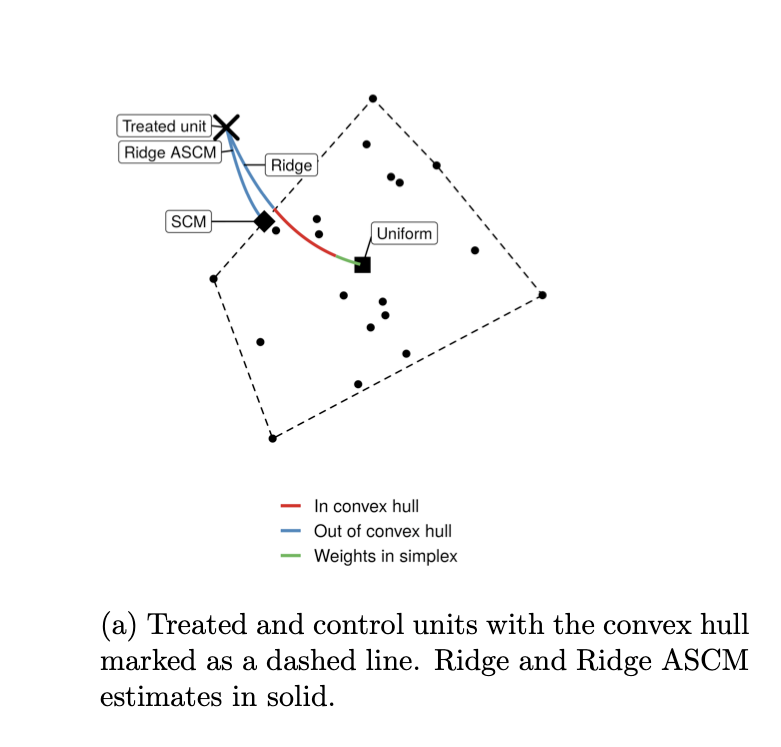
\includegraphics[scale=0.5]{./lecture_includes/aug_1.png}
	\end{figure}
	
\end{frame}	


\begin{frame}{Conformal Inference}

Inference will be based on ``conformal inference'' method by Chernozhukov et al. (2019).  We will get 95\% point-wide confidence intervals. They also outline a jackknife method by Barber et al (2019). 

\end{frame}


\begin{frame}{Steps of conformal Inference}

\begin{enumerate}
\item [1] Choose a sharp null (i.e., no unit-level treatment effects, $\delta_0=0$)
	\begin{itemize}
	\item Enforce the null by creating an adjusted post-treatment outcome for the treated unit equal to $Y_{1T}-\delta_0$ (in other words, we get CI on the post-treatment outcomes, not the pre-treatment)
	\item Augment the original dataset to include the post-treatment time period $T$ with the adjusted outcome and use the estimator to obtain the adjusted weights $\widehat{w(\delta_0)}$
	\item Compute a p-value by assessing whether the adjusted residual conforms with the pre-treatment residuals (see Appendix A for the exact formula)
	\end{itemize}
\end{enumerate}


\end{frame}


\begin{frame}{Steps of conformal Inference}

\begin{enumerate}
\item [2] Compute a level $\alpha$ for $\delta$ by inverting the hypothesis test (see Appendix A for the exact formula)
	\begin{itemize}
	\item Chernozhukov et al. (2019) provide several conditions for which approximate or exact finite-sample validity of the $p$-values (and hence coverage of the predicted confidence intervals) can be achieved)
	\end{itemize}
\end{enumerate}

See Appendix A for more details

\end{frame}


\begin{frame}{Simulations (summarized)}

\begin{itemize}
\item They examine the performance of synth against ridge, Augmented synth with ridge regularization, demeaned synth, and fixed effects under four DGP
\item Augmenting synth with a ridge outcome regression reduces bias relative to synth alone in all four simulations
\item This underscores the importance of the recommendation Abadie, et al. (2015) make which is that synth should be used in settings with excellent pre-treatment fit
\item They also examine a real situation involving Kansas tax cuts in 2012
\end{itemize}

\end{frame}

\imageframe{./lecture_includes/aug_5.png}

\imageframe{./lecture_includes/aug_6.png}

\begin{frame}{Couple of minor points}

\begin{itemize}
\item Hyper parameter chosen using cross validation
\item This can be extended to auxiliary covariates as opposed to just lagged outcomes (section 6)
\end{itemize}

\end{frame}



\begin{frame}{Some minor points}

\begin{itemize}
\item We've motivated augmented synth as a kind of bias correction, but you can also think of it as correcting synth with an inverse probability weight (Appendix E)
\item There's an implicit estimate of a propensity score model with ridge regularization
\item Weights are odds of treatment (they're ATT weights), i.e., they're the inverse probability weighting scheme from Abadie (2005)
\end{itemize}

\end{frame}


\begin{frame}{Augmented synth vs original synthetic control}

\begin{itemize}
\item In conclusion, synthetic control is best when pre-treatment fit is excellent, otherwise it is biased
\item Synthetic control avoids extrapolation by restricting weights to be non-negative and sum to one
\item Ridge regression augmentation will allow for a degree of extrapolation to achieve pre-treatment balance and that creates negative weights
\item Augmented synth will dominate synth in those instances by extrapolating outside the convex hull
\item They also say synth DiD is a special case of their augmented synth method, which is interesting as synth DiD is also meant to nest all such modifications too (but they don't discuss augmented synth)
\end{itemize}

\end{frame}



\begin{frame}{R code}

R: \url{https://github.com/ebenmichael/augsynth}

\end{frame}


\section{Multiple Treated Units and Staggered}

\subsection{Matrix completion with nuclear norm}

\begin{frame}{Big idea}

\begin{quote}
``The main part of the article is about the statistical problem of imputing the missing values of $Y$.  Once these are imputed, we can estimate the causal effect of interest, $\delta$.''
\end{quote}

\bigskip

\begin{quote}
``To estimate average causal effect of the treatment on the treated units, we impute the missing potential control outcomes'' -- Athey, et al. (2021)
\end{quote}


\end{frame}

\begin{frame}{Overview}

\begin{itemize}
\item Athey, et al. (2021) unites two literatures -- unconfoundedness and synthetic control
\item Combines computer science with statistics to create the matrix completion with nuclear norm (MCNN) estimator
\item Nuclear norm regularization is used for the imputation
\end{itemize}

\end{frame}

\begin{frame}{What is matrix completion}

\begin{itemize}
\item Completing a matrix means guessing at the correct values that are missing 
\item Hence the ``completion'' is just another name for ``filling in'' the matrix 
\item In causal inference, if the matrix is a matrix of potential outcomes (e.g., $Y^0$), then missingness is caused by treatment assignment
\end{itemize}
\end{frame}

\begin{frame}[plain]


Here's a matrix of potential outcomes, $Y^0$, representing units at time $t$ that had not been treated. 
\begin{center}
\[ Y^0_{it}  =\begin{pmatrix}
    Y^0_{11} & Y^0_{12} & Y^0_{13} & \dots  & Y^0_{1t} \\
    Y^0_{21} & Y^0_{22} & Y^0_{23} & \dots  & Y^0_{2t} \\
    \vdots & \vdots & \vdots & \ddots & \vdots \\
    Y^0_{i1} & Y^0_{i2} & Y^0_{i3} & \dots  & Y^0_{it}
\end{pmatrix}\]
\end{center}

Now imagine a treatment assignment, SUTVA, that flips treatment from 0 to 1 in the last period $t$:

\begin{eqnarray*}
Y=DY^1 + (1-D)Y^0
\end{eqnarray*}

\end{frame}

\begin{frame}[plain]

Ask yourself: why are there question marks in the last column? 

\begin{center}
\[ Y^0_{it}  =\begin{pmatrix}
    Y^0_{11} & Y^0_{12} & Y^0_{13} & \dots  & ? \\
    Y^0_{21} & Y^0_{22} & Y^0_{23} & \dots  & ? \\
    \vdots & \vdots & \vdots & \ddots & \vdots \\
    Y^0_{i1} & Y^0_{i2} & Y^0_{i3} & \dots  & ?
\end{pmatrix}\]
\end{center}
Matrix completion seeks to do the following:



\end{frame}


\begin{frame}[plain]

Matrix completion with nuclear norm will impute the last column using regularized regression:

\begin{center}
\[ Y^0_{it}  =\begin{pmatrix}
    Y^0_{11} & Y^0_{12} & Y^0_{13} & \dots  & \widehat{Y^0_{1t}} \\
    Y^0_{21} & Y^0_{22} & Y^0_{23} & \dots  & \widehat{Y^0_{2t}} \\
    \vdots & \vdots & \vdots & \ddots & \vdots \\
    Y^0_{i1} & Y^0_{i2} & Y^0_{i3} & \dots  & \widehat{Y^0_{it}}
\end{pmatrix}\]
\end{center}

And once you have those, you can calculate individual level treatment effects that can be used to aggregate to the ATT

\end{frame}


\begin{frame}{History of matrix completion}

\begin{itemize}
\item Open competition by Netflix in 2006 -- winner would get \$1m if they could improve predictive model by ten points on RMSE
\item Invited a ton of competition -- from MIT teams to regular everyday joes working out of their home office
\item Everyone was given a database which was then tested by Netflix on a holdout dataset
\item Quick progress was made followed by very slow advances
\item Winner was announced in 2009
\end{itemize}

\end{frame}

\begin{frame}{Netflix prize}

\begin{itemize}
\item Gigantic sparsely populated matrix (100m users ranking 100k movies)
\item I like \underline{Silver Linings Playbook} and \underline{Lars and the Real Girl} and you like \underline{Silver Linings Playbook}
\item Probably you'll also like \underline {Lars and the Real Girl}
\item So we are using correlations in the columns to ``complete'' missing values
\item When you think about it, while it seems predictive (and it is), isn't it really a causal design?
\item ``If I watch \underline{Lars and the Real Girl}, will I like it?''
\end{itemize}

\end{frame}

\begin{frame}{Types of imputation}

\begin{itemize}
\item I didn't always think of causal inference in terms of imputation because often the method was just taking existing values and manipulating them, rather than filling in missing values
\item But the fundamental problem of causal inference states that causal inference is a missing data problem, so it makes sense you'd be imputing
\item I tend to think therefore in terms of implicit and explicit imputation methods
\item Borusyak, et al. (2021) and Athey, et al. (2021) both seem more like ``explicit'' imputation methods
\item Callaway and Sant'Anna (2020) on the other hand is an implicit method, as is did methods more generally
\end{itemize}

\end{frame}

\begin{frame}{Two literatures}

\begin{itemize}
\item Lots of moving parts in this interesting paper, so my goal here is purely explainer and mostly high level at that. 
\item I want you to be competent and conversant in it so we also have some R code
\item There's two literatures they want you to have in your mind:
	\begin{enumerate}
	\item Unconfoundedness -- $(Y^0,Y^1)\independent D|X$ -- sometimes explicitly imputes (nearest neighbor), sometimes more implicit (inverse probability weighting)
	\item Synthetic control -- literally calculating a counterfactual as a weighted average over all donor pool units
	\end{enumerate}
\item Their MCNN method will show that both are ``nested'' within the general framework they've developed making them actually special cases
\end{itemize}

\end{frame}


\begin{frame}{Differences}

\begin{itemize}
\item Conceptually different in the way they exploit patterns for causal inference
\item Unconfoundedness assumes that \textbf{patterns over time}are stable \emph{across units}
\item Synth assumes \textbf{patterns across units} are stable \emph{over time}
\item Regularization nests them both
\item Nuclear norm ensures a low rank matrix needed for sensible imputations

\end{itemize}

\end{frame}

\begin{frame}{The Gist}

\begin{itemize}
\item Factor models and interactive effects model the observed outcome as the sum of a linear function of covariates and a unobserved component that is a low rank matrix plus noise
\item Estimates are typically based on minimizing the sum of squared errors given the rank of the matrix of unobserved components with the rank itself estimated
\item Nuclear norm regularization will be used for imputing the potential outcomes, $Y^0$, for all treated units
\item Estimate plots and overall ATT using the estimated treatment effects
\end{itemize}

\end{frame}

\begin{frame}{Three contributions}

\begin{enumerate}
\item Formal results for non-random missingness when block structure allows for correlation over time.  Nuclear norm is important here
\item Shows unconfoundedness and synth are in fact matrix completion methods 
	\begin{itemize} 
	\item they all have the same objective function based on the Frobenius norm for the difference between the latent matrix and the observed matrix
	\item Each approach imposes different sets of restrictions on the factors in the matrix factorization
	\item MCNN by contrast doesn't impose any restrictions -- just regularization to characterize the estimator
	\end{itemize}
\item Applies the method to two datasets, but I'm going to skip it though for now
\end{enumerate}

\end{frame}


\begin{frame}{Block structure}

\begin{itemize}
\item Lots of jargon in this article -- unconfoundedness, vertical and horizontal regression, fat and thin matrices.  
\item Unfortunately, you need to learn it all so let me try and organize it
\item We define the matrix first in terms of its block structure which is describing where and when the missingness is occurring in the matrix
\end{itemize}

\end{frame}

\begin{frame}{Unconfoundedness}

\begin{itemize}
\item Much of the unconfoundedness literature estimates an ATE under unconfoundedness 
\item But it tends to focus only on a simple setup where the missingness is the last period
\item Think about LaLonde (1986) -- NSW treats the workers, and then you don't observe $Y^0$ for the treated group in the \emph{last period}
\item This is the ``single-treated-period block structure'' because only one \emph{period} is missing
\end{itemize}

\end{frame}

\begin{frame}{Single-treated-period block structure}

\begin{center}
\[ Y^0_{it}  =\begin{pmatrix}
    Y^0_{11} & Y^0_{12} & Y^0_{13} & \dots  & ? \\
    Y^0_{21} & Y^0_{22} & Y^0_{23} & \dots  & ? \\
    \vdots & \vdots & \vdots & \ddots & \vdots \\
    Y^0_{i1} & Y^0_{i2} & Y^0_{i3} & \dots  & ?
\end{pmatrix}\]
\end{center}

\end{frame}


\begin{frame}{Single-treated-unit block structure}

\begin{center}
\[ Y^0_{it}  =\begin{pmatrix}
    Y^0_{11} & Y^0_{12} & Y^0_{13} & \dots  & Y^0_{1t} \\
    Y^0_{21} & Y^0_{22} & Y^0_{23} & \dots  & Y^0_{2t}  \\
    \vdots & \vdots & \vdots & \ddots & \vdots \\
    Y^0_{i1} & Y^0_{i2} & ? & \dots  & ?
\end{pmatrix}\]
\end{center}

Notice, this is the synthetic control design because a single unit (unit $i$) is missing $Y^0$ for the 3rd and $t$th periods.

\end{frame}

\begin{frame}{Staggered adoption}

\begin{center}
\[ Y^0_{it}  =\begin{pmatrix}
    Y^0_{11} & ? & ? & \dots  & ? \\
    Y^0_{21} & Y^0_{22} & Y^0_{23} & \dots  & ? \\
    \vdots & \vdots & \vdots & \ddots & \vdots \\
    Y^0_{i1} & Y^0_{i2} & ? & \dots  & ?
\end{pmatrix}\]
\end{center}

So all of these so-called designs can be expressed in terms of missingness in the block structure, and our job therefore is to find an estimator that is general enough to manage all of them.  Their MCNN will be that.

\end{frame}


\begin{frame}{Thin and Fat matrices}

\begin{itemize}
\item We also have to consider the relative number of panel units $N$ and time periods $T$ because this also shapes which regression style will be used for imputation
\item Thin matrices are basically where $N>>T$, but fat matrices are ones where $T>>N$
\item Approximately square ones are where $T$ is approximately equal to $N$
\end{itemize}

\end{frame}


\begin{frame}{Vertical and horizontal regression}

\begin{itemize}
\item Two special combinations of missing data patterns and matrix shape need special attention because they are the focus of large but separate literatures
\item Unconfoundedness has that single-treated period block structure with a thin matrix ($N>>T$). 
\item You use a large number of units and impute missing potential outcomes in the last period using controls with similar lagged outcomes
\item This is the horizontal regression -- imagine just running OLS on the lags and taking predicted values
\item The horizontal regression holds under unconfoundedness
\end{itemize}

\end{frame}

\begin{frame}{Vertical regression}

Doudchenko and Imbens (2016) and Pinto and Furman (2019) show that Abadie, Diamond and Hainmueller (2011) can be interpreted as regressing the outcomes for the treated prior to treatment on the outcomes for controls in the same period

\end{frame}

\begin{frame}{Fixed effects and factor models}

\begin{itemize}
\item Both horizontal and vertical regressions exploit other patterns
\item An alternative to each of them though is to consider an approach that allows for the exploitation of both stable patterns over time and stable patterns across units
\item This is where their matrix completion with nearest neighbor model comes in -- it does that very thing
\end{itemize}

\end{frame}

\begin{frame}{Matrix completion with nuclear norm}

\begin{itemize}
\item Model the $N \times T$ matrix of complete outcomes data matrix $Y$ as: $$Y = L* + e$$where $E[e|L*]=0$
\item The error term can be thought of as measurement error if you need a frame to think about it
\item So you have this complete matrix, L*, and zero mean conditional independence holds
\end{itemize}

\end{frame}

\begin{frame}{Assumption 1}

Apart from the unconfoundedness assumption, we have this weird assumption!

\begin{block}{Assumption 1}
$e$ is independent of $L*$ and the elements of $e$ are $\sigma$-sub-Gaussian and independent of each other
\end{block}

Lots of matrix forms can be defined this way.  But let's not get lost in the weeds -- we are still just trying to estimate $L*$!  That's the main storyline, not the side quest, to use Red Dead Redemption words I understand

\end{frame}

\begin{frame}{All imputations are wrong but some are useful}	
	
\begin{itemize}
\item You can impute something a million different ways.  
\item $1+1+1+1 = 4$ is an imputation of the fifth unknown element and frankly just looking at it, seems wrong.
\item You could minimize the sum of squared differences but if the objective function doesn't depend on $L*$, the estimator would just spit back $Y$ and $\delta=0$. 
\item They add a penalty term $||\lambda||$ to the objective function, but even then, not all of them do well. 
\item Turns out, it actually matters whether you regularize the fixed effects or not (just like it matters whether you regularize the constant in LASSO apparently -- I decided to take their word for it)
\end{itemize}

\end{frame}

\begin{frame}{Estimator}

\begin{eqnarray*}
L* = \widehat{L} + \widehat{\Gamma}1_T^T + I_N\widehat{\Delta}^T
\end{eqnarray*}where the objective function is:

\begin{eqnarray*}
= arg\text{ }min_{L,\Gamma,\Delta} \bigg \{ \frac{1}{O} || P_0(Y-L-\Gamma 1_T^T - 1_N\Delta^T)||_F^2 + \Lambda||L|| \bigg \}
\end{eqnarray*}

\end{frame}

\begin{frame}{Fixed effects and regularization}

\begin{itemize}
\item The penalty will likely be the nuclear norm but notice that the fixed effects are outside the penalty term.  You could subsume them into $L$, they say, but they recommend you not doing this.
\item Fraction of observations is relatively high and so the fixed effects can actually be estimated separately (apparently that is one difference between MCNN and the rest of the MC literature)
\item The penalty will be chosen using cross-validation
\end{itemize}

\end{frame}

\begin{frame}{Other norms}

\begin{itemize}
\item One thing I thought was interesting was that the nuclear norm allowed for the construction of a low rank $L*$ matrix, but other norms actually would have weird properties
\item I remember once me asking Imbens (like I had even a clue what I was talking about), ``Why not use elastic net?  Why are you using the nuclear norm?'' He said elastic net would spit out all zeroes.  I remember thinking ``Why did I think I would understand what he told me?''
\item One advantage of NN is its fast and convex optimization programs will do it, whereas some others won't because of the large $N$ or $T$ issues
\item There's almost like a cross walk, too, between this and Borusyak, et al. (2021) but I don't quite see it except they both leverage imputation
\end{itemize}
\end{frame}

\begin{frame}{Conclusion}

\begin{itemize}
\item Ultimately, this is just another model though that can be used for differential timing but at the moment, no one knows how it performs in simulations alongside Borusyak, et al. (2021), Callaway and Sant'Anna (2020) or any of the others
\item So I can't really answer questions about when to use it and not to -- it comes down to these very narrow assumptions
\item You choose the estimator based on the problem you're studying and the assumptions -- you must justify it, no one else can, but you do so by appealing to assumptions
\end{itemize}

\end{frame}

\begin{frame}{Code}

R: \url{https://github.com/xuyiqing/gsynth}

\bigskip

Stata: fect \url{https://yiqingxu.org/packages/fect/stata/fect_md.html}

\end{frame}





\subsection{Synthetic difference-in-differences}

\begin{frame}{New developments}

\begin{itemize}
\item Remember what Athey and Imbens said -- ``most important innovation in causal inference of the last 15 years''.
\item The synthetic DiD bears some similarities to their MCNN model, but focuses on estimating weights, not the $L^*$ matrix
\item It will dominate the Abadie, Diamond and Hainmueller (2010) as they will show and addresses overfitting and other things through estimating oracle weights (which I'll explain towards the latter half)
\end{itemize}

\end{frame}





\begin{frame}{Imperfect fits}

\begin{itemize}
\item Recall that ADH needs to fit a pre-treatment convex hull to model the heterogeneity
\item Often, though, the fit is imperfect for various reason because weights are constrained to be non-negative and sum to one
\item But this can be problematic if the treatment group can't be approximated by a weighted average of other units since the weights are fractions 
\item So they're going to allow for a constant level shift to ``get there''
\end{itemize}

\end{frame}



\begin{frame}{Diff-in-diff, parallel trends and pre-trends}

\begin{itemize}
\item Recall the identifying assumption in DiD -- parallel trends
\item Untestable, but we often use pre-trends for an indirect test
\item But in the smoking example, parallel trends didn't hold for many states
\item Choice of control units matter -- the average trends for many control states are roughly parallel, but not all 
\end{itemize}

	
	\begin{figure}
	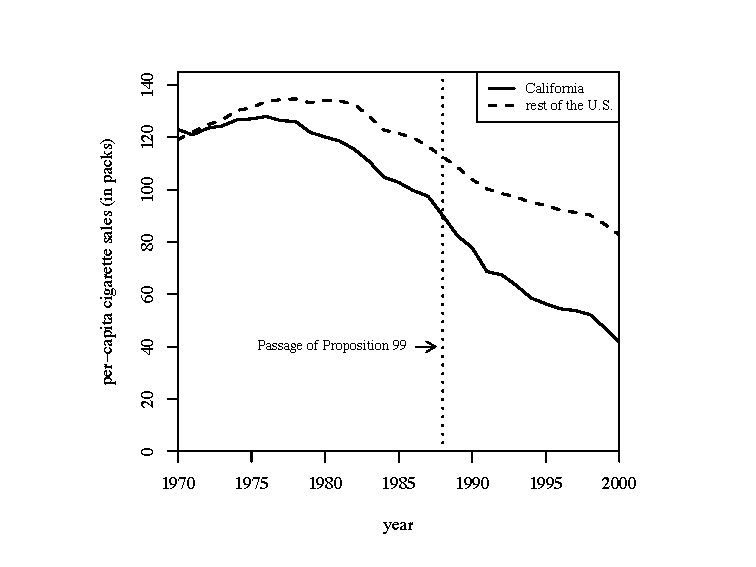
\includegraphics[scale=0.65]{./lecture_includes/abadie_3.pdf}
	\end{figure}


\end{frame}

\begin{frame}{Weights and controls}

\begin{itemize}
\item ADH sought a weighted average over the control units to recreate the pre-trend through a fitting exercise
\item Synthetic control becomes the weighted average of controls, and then the focus is just on estimating weights
\item All we ask is that the weighted average follow the same dynamic path as treatment group (a fit for each period)

\end{itemize}

\end{frame}

\begin{frame}{Regressions up and down}

\begin{itemize}
\item Doudchenko and Imbens (2015) note that synth weights are based on a ``vertical regression'' yielding coefficients on the control units (as opposed to the lags in $T$ which is a horizontal regression)
\begin{eqnarray*}
Y^0_{1,t} = \sum_{j=2}^{J+1} \widehat{\omega_j} \times Y_{j+1,t}
\end{eqnarray*}
\item To the degree the fit is good pre-treatment, then the gaps post-treatment measure ATT at a point in time

\end{itemize}

\end{frame}


\begin{frame}{Weighting across controls}

Assume that the synthetic control at any period is $Y_{1,t} \approx \sum_{j=2}^{J+2} w_i \times Y_{j}$
\begin{itemize}
\item Synthetic control -- weights, $\widehat{w}$, control units to get weighted average controls
	\begin{enumerate}
	\item Use the pre-treatment data to find the optimal weights that when aggregated over control units predict treatment group outcomes (``fit'')
	\item Assumes that there's a stable relationship over time, though, because this is going to be our estimated counterfactual post-treatment
	\end{enumerate}
\item This is shown to be equivalent to a ``vertical regression'' where you regress units against the higher column units to get those weights
\item May require regularization in the regression (if there are more units than time periods)
\end{itemize}

\end{frame}

\begin{frame}{Weighting across time dimensions}

\begin{itemize}
\item Forecasting -- time weights, $\widehat{\lambda}$,  periods to get weighted average periods
	\begin{enumerate}
	\item Use the controls to learn an average of periods that forecast what we see post-treatment
	\item Imagine a regression, in other words, that yields coefficients on covariates, not on units, to predict future counterfactual
	\item Assumes that this relationship remains valid for the treated and we use the same average of periods to impute the $Y^0$ for our treatment group
	\end{enumerate}
\item This is equivalent to a ``horizontal regression'' where you regress outcomes against the leads (i.e., $Y_{it}$ against $Y_{i,t-1}$) -- this is what was meant by unconfoundedness from the MCNN lecture
\item Again may need regularization if there are more time periods than units
\end{itemize}

\end{frame}

\begin{frame}{Difference-in-differences model}

\begin{itemize}
\item They tend to equate DiD with a TWFE model $$Y(0)_{it} = \mu + \alpha_i + \gamma_t + \varepsilon_{it}$$ and solve for the unknown parameters
\item More generally, these are the factor models 
\end{itemize}

\end{frame}

\begin{frame}{Reconciling these things}

\begin{itemize}
\item Vertical regression (i.e., the ADH synth approach) assumes there is a stable relationship between units over time (hence why the weights accurately estimate counterfactuals post-treatment)
\item Horizontal regression (i.e., the unconfoundedness approach) is similar, but assumes a stable relationship between outcomes in the treatment period and pre-treatment periods that is the same for all units
\item DiD regression (TWFE): assumes an additive outcome model that captures differences between time and units
\end{itemize}

\bigskip

So the focus becomes about choosing between these methods

\end{frame}



\begin{frame}{Synthetic DiD}

Synthetic DID takes synth and forecasting to create a \emph{synthetic DiD} version
\begin{itemize}
\item Combine these two -- weighting controls using pre-treatment and weighting time using controls, then applying a type of DiD differencing -- to create the synthetic DiD model
\item There is a focus, just like ADH, on estimating appropriate weights
\item It's doubly robust -- only one has to remain valid
\item Constant effects will get differenced out and the synthetic control can be \emph{parallel} to treatment, as opposed to \emph{identical} in pre-treatment period
\end{itemize}

\end{frame}


\begin{frame}{Estimation of SDiD}

Synthetic DiD is DiD with a synthetic control and a pre-treatment period (on the baseline, just like CS). 
	\begin{enumerate}
	\item[1. ] Compute the regularization parameter to match the size of a typical one-period outcome change, $\Delta_{it} = Y_{i(t+1)} - Y_{it}$, for unexposed 
	\end{enumerate}

\end{frame}


\begin{frame}{Estimation of SDiD}

	\begin{enumerate}

	\item[2. ] Estimate unit weights $\widehat{w}$ defining a synthetic control unit (just like Abadie, Diamond and Hainmueller 2010) using the pre-treatment data $$\widehat{w}_1 + \widehat{w}^TY_{j,pre} \approx Y_{1,pre}$$ but they allow for an intercept term so that now the weights no longer need to make the unexposed pre-trends \emph{perfectly} match the treatment group (hence convex hull can fail to hold)
	\end{enumerate}

\end{frame}

\begin{frame}{Estimation of SDiD}

	\begin{enumerate}

	\item[3. ] Estimate the time weights $\widehat{\lambda}$ defining a synthetic pre-treatment period using control data$$\widehat{\lambda}_{j=1} + Y_{1,pre} \widehat{\lambda} \approx Y_{1,post}$$
	\end{enumerate}

\end{frame}


\begin{frame}{Estimation}

\begin{enumerate}
\item[4. ] Compute the SDID estimator via the weighted DID regression
\end{enumerate}

\begin{eqnarray*}
\textrm{arg min}_{\tau, \mu, \alpha, \beta} = \bigg \{ \sum_{i=1}^N \sum_{t=1}^T ( Y_{it} - \mu - \alpha_i -\beta_t - W_{it}\tau ) ^2 \widehat{w}_i^{sdid} \widehat{\lambda_t}^{sdid}  \bigg \}
\end{eqnarray*}


\end{frame}

\begin{frame}{Estimating the weights}

Our focus then becomes about estimating $\widehat{w}$ and $\widehat{\lambda}$

\begin{enumerate}
\item[5. ] Estimate the control weights, $\widehat{w}$, defining the control group unit via constrained least squares on the pre-treatment data. This requires weights to be non-negative and sum to one and allows for a level shift with regularization.  Synthetic control is a weighted average like in ADH
\end{enumerate}

\end{frame}


\begin{frame}{Estimating the weights}

\begin{enumerate}

\item[6. ] We then estimate the time weights. $\widehat{\lambda}$, defining the synthetic pre-treatment period via constrained least squares on the control data with analogous time constraints

\end{enumerate}

\end{frame}






\begin{frame}{More formalization}


Assumed data generating process -- outcome is ``low rank matrix'' (MCNN) plus noise

\bigskip


\begin{eqnarray*}
Y = L + \tau D  + E
\end{eqnarray*}

\bigskip

where $L$ is the systematic component and the conditional expectation of the error matrix $E$ given the assignment matrix $D$ and the systematic component of $L$ is zero.  

\bigskip

We won't estimate $L^*$ though, unlike MCNN

\end{frame}


\begin{frame}{Data generating process -- noise and signal}

\begin{eqnarray*}
Y = L + \tau D  + E
\end{eqnarray*}

\bigskip

The treatment cannot depend on the error term, but may depend on the systematic elements of $L$ (i.e., $D$ is not randomized). Think of $L$ as the signal, $\tau$ a matrix of treatment effects and $E$ the noise with no autocorrelation over time or between units. The only thing random is $E$, our noise matrix.

\end{frame}

\begin{frame}{Estimating the weights -- high level}

\begin{itemize}
\item Modify synthetic control weights -- use penalized least squares to get a weighted average of control units with pre-trends ``parallel'' to the treated unit average
\item But they'll allow for a constant, unlike ADH synth
\item And then they'll do the same thing for the time weights, but this time they won't regularize because they want to weight more intensively the periods ``just before'' -- ridge, they note, would ``spread out the weights'' over multiple time periods and they don't want that
\item I'll get more into this with the oracle weights, but for now I'll just note it conceptually
\end{itemize}

\end{frame}

\begin{frame}{Picture}

	\begin{figure}
	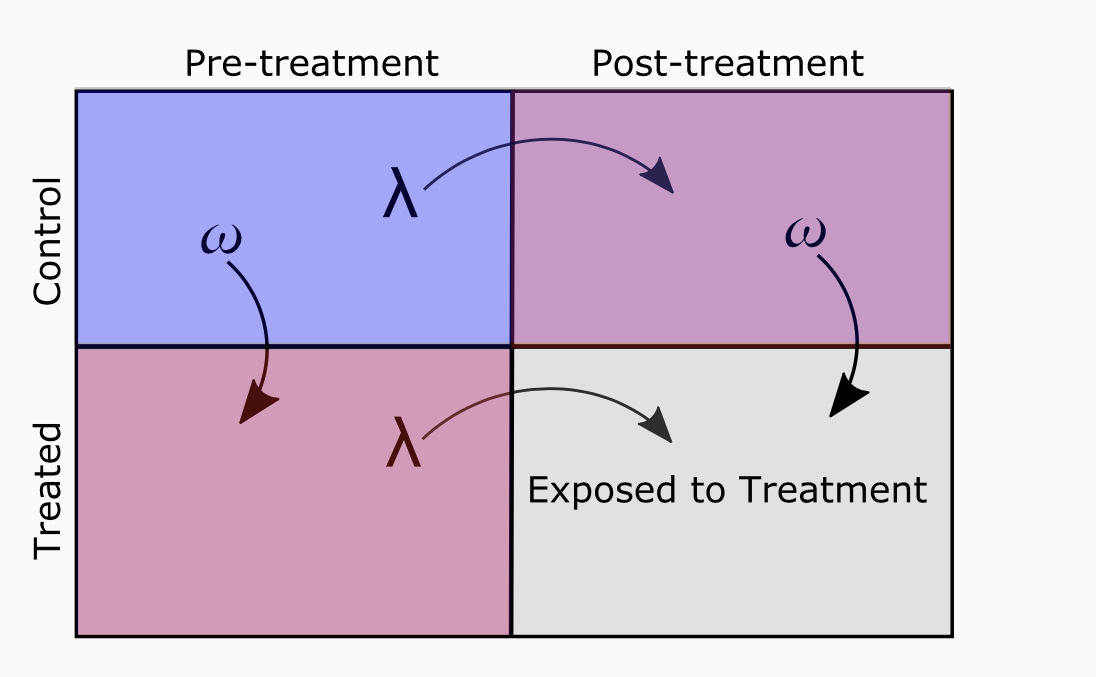
\includegraphics[scale=0.3]{./lecture_includes/hirshberg_sdid_1.png}
	\end{figure}

(credit: David Hirshberg January 2020 slides because I can't make this picture to save my life)

\end{frame}

\begin{frame}{Regression}

\begin{itemize}
\item SC is weighted linear regression with no unit FEs:$$\tau^{sc} = \textrm{argmin}_{\tau, \lambda}  \sum_{i,t} (Y_{it} - \lambda_t - \tau D_{it})^2 \times w_i^{sc} $$
\item DiD is unweighted regression with unit FEs and time FEs:$$\textrm{argmin}_{\tau, \lambda, \alpha}  \sum_{i,t} (Y_{it} - \lambda_t - \alpha_i -  \tau D_{it})^2 $$
\item SDiD is weighted regression with unit FEs and time FEs:$$ \textrm{argmin}_{\tau, \lambda, \alpha} \sum_{i,t} (Y_{it} - \lambda_t - \alpha_i - \tau D_{it})^2 \times w_i \times \lambda_t$$
\end{itemize}

\end{frame}

\begin{frame}{Formal results overview}

\begin{itemize}
\item Formal results will show SDiD is ``doubly robust'' (recall Sant'Anna and Zhao 2020)
\item Factor model  on the outcome can be a latent factor model but true model is that signal model and it'll still be consistent
\item Asymptotic normality of $\widehat{\tau}^{SDiD}$
\item With oracle weights, SDiD will have ``good weights''
\item You can do inference through resampling like jackknife, bootstrap and randomization inference
\end{itemize}

\end{frame}


\begin{frame}[plain]

	\begin{figure}
	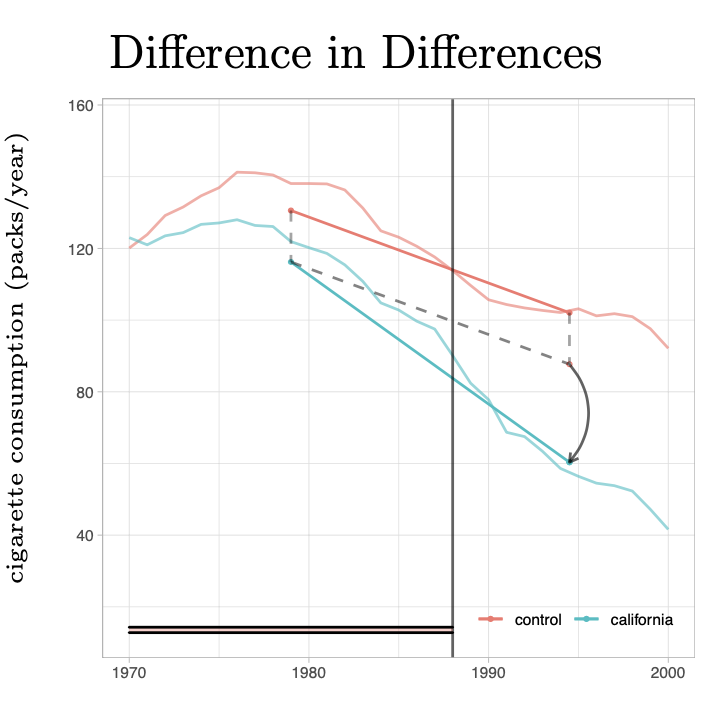
\includegraphics[scale=0.65]{./lecture_includes/sdid_2.png}
	\end{figure}
	
Estimated decrease: -27.3 (17.7)

\end{frame}


\begin{frame}[plain]

	\begin{figure}
	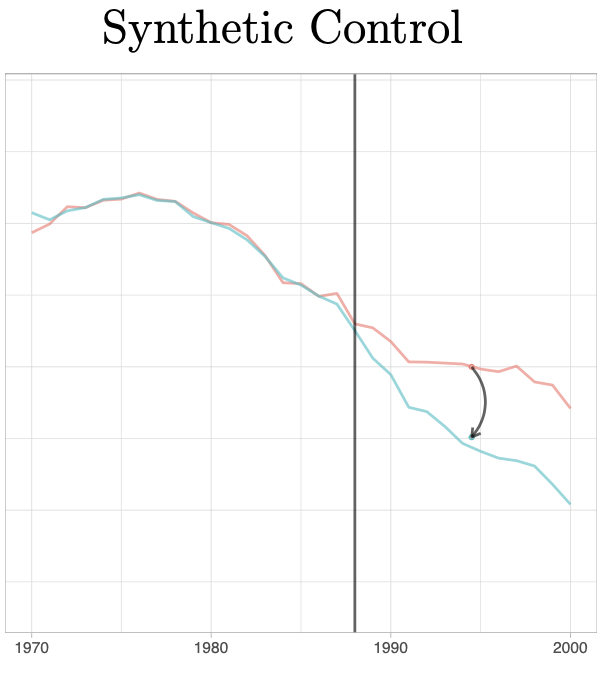
\includegraphics[scale=0.65]{./lecture_includes/sdid_1.png}
	\end{figure}

Estimated decrease: -19.6 (9.9); bad fit just prior bc weights are fitting everywhere

\end{frame}

\begin{frame}[plain]

	\begin{figure}
	\includegraphics[scale=0.65]{./lecture_includes/sdid_3.png}
	\end{figure}
	
Estimated decrease: -15.4 (8.4). Jagged line left of 1988 is the weighting of those years 	

\end{frame}






\begin{frame}{Practical problems}


\begin{itemize}
\item Underfitting. What if I can't get a parallel synthetic control?  I know because it's visible. This is an underfitting problem.  We need more controls, better controls, or another method. 
\item Omitted variable bias.  Something else happens exactly when the treatment occurs.  Sorry -- there isn't a solution, because you're not identified. 
\item Overfitting. We get a synthetic control, but it's because the plot over fit the data. This means that you've not approximated the counterfactual post-treatment.  No different than in RDD when you're unable to identify the counterfactual due to functional form problems. 
\end{itemize}

\end{frame}

\begin{frame}{How to rule out overfitting: oracle weights}

\begin{itemize}
\item Their estimator is equivalent to an ``oracle estimator'' which cannot overfit
\item Oracle uses unit and time weights that don't depend on the noise
\item Weights minimize MSE; oracle weights minimize \textbf{expected} SE
\end{itemize}

\end{frame}

\begin{frame}{Decomposing the bias of SDID}

\begin{eqnarray*}
\widehat{\tau}^{sdid} - \tau  &=& \varepsilon(\widetilde{w}, \widetilde{\lambda}) + B(\widetilde{w}, \widetilde{\lambda}) + \widehat{\tau}(\widehat{w},\widehat{\lambda}) - \widehat{\tau}(\widetilde{w},\widetilde{\lambda}) \\
&=& \textrm{oracle noise} +  \\
&& \textrm{oracle confounding bias} + \\
&&\textrm{deviation from oracle}
\end{eqnarray*}

\bigskip

So they characterize these terms

\end{frame}


\begin{frame}{Oracle noise}

First term: the oracle noise

\bigskip

\begin{eqnarray*}
\varepsilon(\widetilde{w}, \widetilde{\lambda})
\end{eqnarray*}

\bigskip

Tends to be small when the weights are small and there are a sufficient number of exposed units and time periods. 

\end{frame}

\begin{frame}{Oracle confounding bias (rows / units)}

\begin{eqnarray*}
B(\widetilde{w}, \widetilde{\lambda}) 
\end{eqnarray*}

\bigskip

Will be small when the pre-exposure oracle row (units) regression fits well and generalizes to the exposed rows :
 
 $$\widetilde{w_1} + \widetilde{w_{j}}^TL_{j,pre} \approx \widetilde{w}_1^TL_{1,pre}$$and
 
 $$\widetilde{w_1} + \widetilde{w_{j}}^TL_{j,post} \approx \widetilde{w}_1^TL_{1,post}$$
 
 \end{frame}
 
 \begin{frame}{Oracle confounding bias (columns / time)}

\begin{eqnarray*}
B(\widetilde{w}, \widetilde{\lambda}) 
\end{eqnarray*}

\bigskip

Will be small when the pre-exposure oracle column (time) regression fits well and generalizes to the exposed columns :
 
 $$\widetilde{\lambda_1} + \widetilde{\lambda_{j}}^TL_{j,pre} \approx \widetilde{\lambda}_1^TL_{1,pre}$$, and
 
 $$\widetilde{\lambda_1} + \widetilde{\lambda_{j}}^TL_{j,post} \approx \widetilde{\lambda}_1^TL_{1,post}$$
 
 \end{frame}


\begin{frame}{Oracle confounding bias -- neither do well}

What if neither model generalizes well on its own, then there is a doubly robust property

\bigskip

It is sufficient for one model to predict the generalization error of the other

\bigskip

``The upshot is even if one of the sets of weights fails to remove the bias from the presence of $L$, the combination of oracle unit and time weights can compensate for such failures''

\end{frame}

\begin{frame}{Deviation from Oracle}

Core theoretical claim (All formalized in their asymptotic analysis): SDID estimator will be close to the oracle when

\begin{itemize}
\item  The oracle time and unit weights look promising on their respective training sets

\begin{eqnarray*}
\widetilde{w_1} + \widetilde{w_j}^TL_{j,pre} \approx \widetilde{w}_1^T L_{1,pre} \\
\widetilde{\lambda_1} + \widetilde{\lambda_j}^TL_{j,pre} \approx \widetilde{\lambda_1}^T L_{1,pre} 
\end{eqnarray*}

\item and regularization is not too large for either weight
\end{itemize}

\end{frame}

\begin{frame}{Properties}

Under some assumptions, they provide then that SID:

\begin{enumerate}
\item SDiD is approximately unbiased and normal
\item SDiD has a variance that is optimal and estimable via clustered bootstrap
\end{enumerate}


\end{frame}




\begin{frame}{Placebo Simulation}

\begin{itemize}
\item Big picture still -- they do a simulation to evaluate bias, RMSE of estimates compared to the observed outcome, but they don't want to use randomization because that may not catch the distinct time trend
\item They want the simulation to be ``realistic'' not ``ideal'' (i.e., design based identification using randomized treatment dates)
\item  Bertrand, et al. (2004)  randomly assigned a set of states in the CPS to a placebo treatment and the rest the control and examine how well different approaches to inference for DiD covered the true effect of zero
\item Only methods that were robust to serial correlation of repeated observations for a given unit (e.g., clustering by level of treatment) attained valid coverage
\end{itemize}

\end{frame}



\begin{frame}{Treatment assignment process}

\begin{itemize}
\item Policy: abortion laws, gun laws, minimum wages with outcome hours and unemployment rate
\item Logistic regression to predict presence of regulation on four state factors from simulation outcome model $M$
\item Goodness of fit shows that treatment assignment responds strongly to unobserved latent factors
\item Assign treatment to states with probabilities from the logistic model
\end{itemize}

\end{frame}



\begin{frame}{Some details of this placebo simulation}

\begin{itemize}
\item They calculate average earnings over 40 years and 50 states by subtracting the overall mean and dividing by the standard deviation to get a matrix $Y$ with $||Y||^2_2 = 1$
\item They fit a rank 4 factor model $M$ 
\item They then extract TWFE from there based on unit and time fixed effects $F$
\item Extract low rank matrix as  $L=M-F$
\item Calculate residuals $E=Y-M$ on an AR(2) model
\item Compared SDID, DiD, synthetic control and matrix completion under different baseline scenarios and SDID tends to better

\end{itemize}

\end{frame}


\imageframe{./lecture_includes/sdid_5.png}


\imageframe{./lecture_includes/sdid_4.png}


\begin{frame}{Inference}


This can be used to motivate practical methods for large-sample for inference.  You can use conventional confidence intervals to conduct asymptotically valid inference, and they discuss three ways: jackknife, bootstrap, and placebo variance estimation.

\end{frame}





\imageframe{./lecture_includes/sdid_7.png}

\begin{frame}{Some practical considerations}

More treated units is worse -- when we add treated units, the oracle standard deviation decreases faster leaving too little room for other sources of error to disappear in the noise

\end{frame}

\begin{frame}{More practical considerations}

Circumstances are ideal if the signal matrix $L$ admits a good oracle synthetic control and synthetic pre-treatment period and it's too complex

	\begin{itemize}
	\item What is good?  Oracle control weights distribute mass over enough control units
	\item Oracle time weights should distribute the rest of its mass over enough time periods
	\end{itemize}


\end{frame}

\begin{frame}{More practical considerations}

Interestingly, this is an overlap assumption (like common support in matching and CS DiD):
	\begin{itemize}
	\item Many control units are like the treated ones
	\item Many pre-treatment periods are comparable to post-treatment ones
	\end{itemize}

\end{frame}


\begin{frame}{More practical considerations}

What is ``not too complex'' signal matrix $L$? It's one that looks different from the matrix of noise

\begin{itemize}
	\item More about the rank of the matrix -- it must be moderate rank
	\item Moderate means smaller than the square root of the number of control units
	\item A state's behavior isn't idiosyncratic, but characterized by a blend of industries, etc. of relatively few trends
\end{itemize}

\end{frame}


\begin{frame}{More practical considerations}

\begin{itemize}
\item Including more controls won't hurt you bc the set of weights is small and the error is insensitive to dimension
\item Less than ideal circumstances can be problematic. The error gets worse:
	\begin{itemize}
	\item Signal is too complex
	\item Fit and dispersion of the oracle weights is poor
	\end{itemize}
\end{itemize}

\end{frame}


\begin{frame}{Some comments}

\begin{itemize}
\item Conceptually, this is ADH synth combined with a simple 2x2 DiD where the weights are based on estimated time and control group weights
\item Oracle weights will make improvements that don't suffer from some of the practical problems, like overfitting, that we said
\item Synth DiD dominates synthetic control
\item Still remains to be seen how we are going to go about choosing between these, but some things we may need to put down (ADH)
\end{itemize}

\end{frame}

\begin{frame}{R code: synthdid}

Let's look at the code together

\bigskip

Code: \url{https://github.com/synth-inference/synthdid} 

\bigskip

Vignettes: \url{https://synth-inference.github.io/synthdid/articles/more-plotting.html}

\end{frame}

\begin{frame}{Application: Melo, Neilson and Kemboi 2023}


``Indoor Vaccine Mandates in US Cities, Vaccination Behavior and COVID-19 Outcomes'' by Vitor Melo, Elijah Neilson and Dorothy Kemboi, 2023 working paper

\bigskip

Study investigates the effect of city-level vaccine mandates (implemented in US cities) on COVID-19 cases, deaths or vaccine uptake in the cities

\bigskip

Authors use Arkhangelsky, et al. (2021) ``synthetic difference-in-differences'', as well as conventional synthetic control and difference-in-differences and finds no effect of either the announcement or implementation of the mandate had any significant effect on the outcomes

\end{frame}

\begin{frame}{Motivation}

\begin{itemize}
\item Many policies and strategies were taken to incentivize citizens to get vaccinated and reduce COVID-19 spread
\item Indoor vaccine mandates, one of the more restrictive, prevented people from entering public places (e.g., theaters, restaurants) without proof of vaccination
\item Many large cities (NYC, San Francisco, LA, Seattle, Boston, Philadelphia) implemented with the stated goal to raise vaccination rates and slow spread and mortality from COVID-19
\end{itemize}

\end{frame}

\begin{frame}{Motivation}

\begin{itemize}
\item Vaccine viewed as crucial step toward controlling the virus and return life to normal
\item Substantial number of Americans were unwilling to be immunized
\item February 2021, 30\% of adults say they would probably or definite not be vaccinated
\item Low vaccination rates led to measures to increase uptake like mandated vaccination and weekly testing, lotteries, etc.

\end{itemize}

\end{frame}

\begin{frame}{Mandates}

\begin{itemize}
\item August 3, 2021, due to the Delta variant, NYC passed mandate requiring proof of vaccination to enter restaurants, concerts, stadiums and gyms
\item Similar policies were adopted by other major cities soon after (see next table)
\item I'll skip the prior literature for now
\end{itemize}

\end{frame}


\begin{frame}{Timing}


\begin{table}[ht]
\centering
\caption{Timing of Indoor Vaccine Mandates}
\begin{tabular}{lccc}
\toprule\toprule
City          &  Announced &  Implemented &  Repealed \\ \midrule
NYC           & 8/3/21     & 8/16/21       & 3/7/22    \\
San Francisco & 8/12/21     & 8/20/21       & 3/11/22    \\
New Orleans   & 8/12/21     & 8/16/21       & 3/21/22    \\
Seattle       & 9/6/21     & 10/25/21       & 3/1/22    \\
Los Angeles   & 11/8/21     & 11/29/21       & 3/30/22    \\
Philadelphia  & 12/13/21     & 1/3/22       & 2/16/22    \\
Boston        & 12/20/21     & 1/15/22       & 2/18/22    \\
Chicago       & 12/21/21     & 1/3/22       & 2/28/22    \\
DC            & 12/22/21     & 1/15/22       & 2/15/22    \\ \bottomrule\bottomrule
\end{tabular}
\end{table}


\end{frame}

\begin{frame}{Research question}

\begin{itemize}
\item Estimate an ATT for these cities' mandates on vaccination, cases and deaths
\item Data will come from daily county level COVID-19 vaccinations, cases and deaths from the CDC aggregated to MSA by week scaled by US population estimates
\item Main outcomes: Weekly measures of administered first doses of COVID-19 vaccines, cases, and deaths per 100,000 residents
\item Weekly panel from December 21, 2020 to April 18, 2022 for 821 MSAs (they note various issues with data quality required dropping just under 100 MSAs) with 57,470 observations
\end{itemize}

\end{frame}

\begin{frame}[shrink=20]{Descriptive Statistics}

\begin{table}[ht]
\centering \tiny
\caption{Descriptive Statistics}
\begin{tabular}{lccccccccc}
\toprule\toprule
 & \multicolumn{3}{c}{All MSAs} & \multicolumn{3}{c}{Treated MSAs} & \multicolumn{3}{c}{Untreated MSAs} \\ \cmidrule(lr){2-4} \cmidrule(lr){5-7} \cmidrule(lr){8-10}
Variable              & Mean & SD & Median & Mean & SD & Median & Mean & SD & Median \\ \midrule
First Doses per 100,000  & 817.47 & 1,344.30 & 458.98 & 1,253.50 & 1,237.18 & 827.71 & 812.66 & 1,344.65 & 455.01 \\
Cases per 100,000        & 273.75 & 373.61 & 147.73 & 247.47 & 394.75 & 121.95 & 274.04 & 373.37 & 148.16 \\
Deaths per 100,000       & 3.56 & 5.87 & 1.90 & 2.03 & 2.31 & 1.17 & 3.58 & 5.90 & 1.91 \\
Number of observations  & & 57,470 & & & 630 & & & 56,840 & \\ \bottomrule\bottomrule
\end{tabular}
\tiny \newline Notes: The unit of observation is MSA week. Our sample consists of 821 MSAs, 9 of which are treated, and the period spans 70 weeks from December 21, 2020, to April 18, 2022.
\end{table}

\end{frame}


\begin{frame}{Great discussion of synth DiD}


\begin{quote}
``The basic idea is that the unit weights are chosen to find a convex combination of potential control states whose treatment trend in the outcome variable of interest is most parallel to that of the treated state.  The inclusion of the intercept term $\omega_0$ (made possible because of the inclusion of the unit fixed effects) is one way in which the SDID unit weights differ from those of the synthetic control weights.  Instead of the weights needing to make the pre-trend control unit perfectly match that of the treated unit, as is the case with the synthetic control estimator, allowing for this intercept makes it sufficient for the weights to just make the trends parallel.''
\end{quote}

\end{frame}

\begin{frame}[plain]

	\begin{figure}
	\includegraphics[scale=0.3]{./lecture_includes/vitor_table3}
	\end{figure}

\end{frame}


\begin{frame}[plain]

	\begin{figure}
	\includegraphics[scale=0.3]{./lecture_includes/vitor_table4}
	\end{figure}

\end{frame}


\begin{frame}[plain]

	\begin{figure}
	\includegraphics[scale=0.3]{./lecture_includes/vitor_table5}
	\end{figure}

\end{frame}


\begin{frame}[plain]

	\begin{figure}
	\includegraphics[scale=0.3]{./lecture_includes/vitor_figure1}
	\end{figure}

\end{frame}


\begin{frame}[plain]

	\begin{figure}
	\includegraphics[scale=0.3]{./lecture_includes/vitor_figure2}
	\end{figure}

\end{frame}


\begin{frame}[plain]

	\begin{figure}
	\includegraphics[scale=0.3]{./lecture_includes/vitor_figure3}
	\end{figure}

\end{frame}


\begin{frame}{Conclusion}

\begin{itemize}

\item They also report synth and DiD analysis as robustness -- something to keep in mind is the presentation of results are subjective
\item Rather than showing regression results with more controls, we tend to now see different DiD and synth estimators as the robustness
\item Authors fail to find strong evidence the vaccine mandates slowed COVID-19
\item What's your response?

\end{itemize}

\end{frame}






\subsection{Augmented Synthetic Control with Staggered Rollout}

\begin{frame}

\begin{itemize}
\item ADH was designed for a single treated unit, no extrapolation, non-negative weights summed to one
\item Previous Ben-Michael, Feller and Rothstein (2021a) paper addressed imperfect fit in the pre-trends using regularization
\item Ben-Michael, Feller and Rothstein (2021b) focus on the single unit by allowing differential timing
	\begin{itemize}
	\item Augmented synth is a double-robust style (or bias corrected) estimator
	\item This synth is similar to ``shrunken''/empirical Bayes/random effects estimation
	\end{itemize}
\item It sort of fits with the newer differential timing papers, like matrix completion with nuclear norm regularization had, even though neither are technically DiD
\item More machine learning regularization as we've been seeing
\end{itemize}

\end{frame}

\begin{frame}{Paper's Contribution}

\begin{enumerate}
	\item Extend synth to staggered adoption (as opposed to one unit)
	\item Show results using an example of unions on spending
	\item Propensity score weighting with shrinkage
\end{enumerate}

\end{frame}

\begin{frame}{Motivation}


Synthetic control is not a very good propensity score estimator
\begin{itemize}
\item Uses pre-treatment outcomes as covariates (some use other $X$ covariates)
\item Small $N$ and large $K$ means propensity score must be regularized with probability approaching 1 so perfect balance is not achieved
\item You can borrow information to reduce bias from imbalance -- for instance from an outcome model (e.g., a regression) and/or other treated units
\item You can then combine to produced a weighted event study estimator
\end{itemize}

\end{frame}

\begin{frame}{Stepping back}

\begin{itemize}
\item A unit is treated at some period $t$ and we want to know that event's effect on $Y$
\item Standard approach is DiD and event studies
	\begin{itemize}
	\item Tons of papers recently (e.g., Goodman-Bacon 2021, Callaway and Sant'Anna 2020)
	\item But what units all DiD papers is \emph{parallel trends}
	\end{itemize}
\item That assumption may be wrong, in which case the models' findings will be wrong
\end{itemize}

\end{frame}


\begin{frame}{Synth with staggered adoption}

\begin{itemize}
\item Synth was designed originally for the comparative case study -- i.e., one treatment group
\item What do we do when there's more than one treatment group?
\item People in the past tried different things
	\begin{itemize}
	\item If they were all treated at the same time, they'd average the treated units and construct a synthetic control for the average
	\item If it was staggered, then they'd fit synth for each treated unit separately, then average those estimates
	\end{itemize}
\item They're going to propose optimizing a weighted average of the \emph{global balance} (for the average treated unit) and the sum of \emph{unit-specific balance} for each treated unit
\end{itemize}

\end{frame}

\begin{frame}{Intuition}

We want to balance the average of the underlying factor loadings

\begin{itemize}
\item Balancing individual units may cause large imbalance in the average if errors all go in the same direction
\item Balancing the average outcome may not balance factor loadings if imbalance for different treated units offset each other
\end{itemize}

\end{frame}


\begin{frame}{Teacher unions and teacher salaries/spending}

Their application is about teacher unions
\begin{itemize}
\item 1964-1987: 33 states grant collective bargaining rights to teachers
\item Long literature exploited the timing (Hoxby 1996; Lovenheim 2009)
\item Impact on student spending, teacher salaries
	\begin{itemize}
	\item Hoxby (1996) finds increased spending by 12\%
	\item Paglayan (2019) estimates precise zero in an event study model using ever-treated states
	\end{itemize}
\item They're going to re-analyze using all states and synth models
\end{itemize}

\end{frame}



\imageframe{./lecture_includes/augsynth_7.png}

\begin{frame}{Their paper}

\begin{enumerate}
\item \textbf{Methods}: Extend synth to staggered adoption
\item \textbf{Substance}: Application will find minimal effect of unions on spending
\item \textbf{Connection}: Propensity score weighting with shrinkage
\end{enumerate}

\end{frame}



\imageframe{./lecture_includes/augsynth_8.png}

\begin{frame}{Synth treatment effect: average all the synths}

\begin{itemize}
\item Suppose the first $J$ units are treated at times $T_1, \dots, T_J$
\item Suppose we find a synthetic control for each, with $w_{ij}$ the weight on donor unit $i$ for treated unit $j$
\item Our estimate of the ATT at event time $k$ will then be
\end{itemize}

\begin{eqnarray*}
\widehat{\delta} = \frac{1}{J} \sum_{j=1}^{J+1} \bigg ( Y_{j,T_j+k} - \sum_i w_{ij} Y_{i,T_j+k} \bigg )
\end{eqnarray*}Average of $J$ separate synth estimates

\end{frame}


\begin{frame}{Synth treatment effect: average treated unit}

Or, we can think of it as Synth estimate for average treated unit

\begin{eqnarray*}
\widehat{\delta} = \frac{1}{J} \sum_{j=2}^{J+1} Y_{j,T_j+k} - \frac{1}{J} \bigg ( \sum_{j=2}^{J+1} \sum_i w_{ij} Y_{i,T_j+k} \bigg )
\end{eqnarray*}

\end{frame}


\begin{frame}{Two definitions of ATT}


\begin{eqnarray*}
\widehat{\delta} &=& \frac{1}{J} \sum_{j=1}^J \bigg ( Y_{j,T_j+k} - \sum_i w_{ij} Y_{i,T_j+k} \bigg ) \\
&=& \frac{1}{J} \sum_{j=2}^{J+1} Y_{j,T_j+k} - \frac{1}{J} \bigg ( \sum_{j=2}^{J+1} \sum_i w_{ij} Y_{i,T_j+k} \bigg )
\end{eqnarray*}

\end{frame}

\begin{frame}{Optimization problem}

Do we want to optimize the sum of the separate imbalances or the imbalance of the sum (the pooled imbalance)?

\begin{eqnarray*}
\sum_{j=2}^{J+1} || X_j - \sum_i w_{ij}X_i ||^2\textrm{   or  } ||\sum_{j=2}^{J+1} X_j - \sum_i w_{ij} X_i ||^2
\end{eqnarray*}where $j$ is treatment group and $i$ is donor pool units. Notice summations are inside or outside the norm
\end{frame}

\imageframe{./lecture_includes/augsynth_9.png}

\imageframe{./lecture_includes/augsynth_10.png}

\imageframe{./lecture_includes/augsynth_11.png}

\imageframe{./lecture_includes/augsynth_12.png}

\imageframe{./lecture_includes/augsynth_13.png}

\imageframe{./lecture_includes/augsynth_14.png}

\imageframe{./lecture_includes/augsynth_15.png}

\imageframe{./lecture_includes/augsynth_16.png}

\imageframe{./lecture_includes/augsynth_17.png}

\imageframe{./lecture_includes/augsynth_18.png}



\begin{frame}{Proposal: Partially pool synth}

Instead of minimizing pooled imbalance or average state imbalance, minimize a \emph{weighted average}:

\begin{eqnarray*}
\textrm{min  }_{\Gamma \in \Delta^{synth}}  &&v|| \textrm{Pooled balance} ||^2_2 \\
&&+ (1-v) \frac{1}{J} \sum_{j=2}^{J+1} ||\textrm{ State balance } ||^2_2 \\
&&+ \textrm{ penalty }
\end{eqnarray*}``Returns'' to this are highly convex: setting $v$ just a little below 1 yields a big improvement in state-level imbalance with very little cost in pooled imbalance

\end{frame}



\imageframe{./lecture_includes/augsynth_19.png}

\imageframe{./lecture_includes/augsynth_20.png}

\imageframe{./lecture_includes/augsynth_21.png}

\imageframe{./lecture_includes/augsynth_22.png}

\imageframe{./lecture_includes/augsynth_23.png}

\imageframe{./lecture_includes/augsynth_24.png}

\imageframe{./lecture_includes/augsynth_25.png}


\begin{frame}{Augment staggered adoption}

\begin{enumerate}
\item Estimate an outcome model
\item Estimate the partially pooled synth model
\item Use the outcome model to adjust synth for imbalance (bias correction) or alternatively just use synth on the residuals from the outcome model (double robust)
\end{enumerate}

\end{frame}

\begin{frame}{Special case: weighted event study}

\begin{itemize}
\item Estimate unit fixed effects via pre-treatment average: $\overline{Y}_{i,T_j}^{pre}$
\item Estimate synth using residuals (Doudchenko and Imbens 2017; Ferman and Pinto 2018)
\end{itemize}


\begin{eqnarray*}
\widehat{Y}^{aug}_{j,T_j+k}(0) = \overline{Y}_{j,T_j}^{pre} + \sum_{i=1}^N \widehat{w}_{ij} \bigg ( Y_{i,T_j+k} - \overline{Y}_{i,T_j}^{pre} \bigg )
\end{eqnarray*}where $Y(0)=Y^0$

\end{frame}

\begin{frame}{Special case: weighted event study}

Treatment effect estimate is \textbf{weighted diff-in-diff}:

\begin{eqnarray*}
\widehat{\delta}_{jk}^{aug} = \bigg ( Y_{j,T_j+k} - \overline{Y}_{j,T_j}^{pre} \bigg ) - \sum_{i=1}^N \widehat{w}_{ij} \bigg (Y_{i,T_j+k} - \overline{Y}_{i,T_j}^{pre} \bigg )
\end{eqnarray*}Uniform weights correspond to ``standard DiD''

\end{frame}


\begin{frame}[plain]

	\begin{figure}
	\includegraphics[scale=0.4]{./lecture_includes/augsynth_26.png}
	\end{figure}

\end{frame}
\begin{frame}[plain]

	\begin{figure}
	\includegraphics[scale=0.4]{./lecture_includes/augsynth_27.png}
	\end{figure}

\end{frame}
\begin{frame}[plain]

	\begin{figure}
	\includegraphics[scale=0.4]{./lecture_includes/augsynth_28.png}
	\end{figure}

\end{frame}
\begin{frame}[plain]

	\begin{figure}
	\includegraphics[scale=0.4]{./lecture_includes/augsynth_29.png}
	\end{figure}

\end{frame}
\begin{frame}[plain]

	\begin{figure}
	\includegraphics[scale=0.4]{./lecture_includes/augsynth_30.png}
	\end{figure}

\end{frame}
\begin{frame}[plain]

	\begin{figure}
	\includegraphics[scale=0.4]{./lecture_includes/augsynth_31.png}
	\end{figure}

\end{frame}

\begin{frame}{Conclusions}

\begin{itemize}
\item Synth is useful for very difficult problems in which parallel trends is implausible
\item With large $T$ and perfect balance, you can use synth to get approximately unbiased treatment effect estimates under reasonable DGPs (we saw in the original ADH)
\item But perfect balance is a unicorn and doesn't happen in most settings
\item What do we do when it doesn't?  Give up?  Salvage the estimates somehow? How?
\end{itemize}

\end{frame}


\begin{frame}{Conclusions}

\begin{itemize}
\item Augmented synth allows us to salvage the method, using an outcome model to remove bias from imperfect balance
\item Partially pooled synth allows extension to the staggered adoption setting
\item Combining the two methods gives us the best hope 
	\begin{itemize}
	\item A simple fixed effect outcome model leads to a weighted event study
	\item This generalizes recent recommendations for two-way fixed effects
	\end{itemize}
\end{itemize}

\end{frame}





\section{Bonus: Event studies in finance}

\begin{frame}{Possibilities for detecting corruption}

\begin{itemize}

\item Event studies in finance have been used to detect abnormal patterns around ``events'' involving single firms
\item Baker and Gelbach (2020) proposes a type of synthetic control estimator that uses machine learning to estimate a counterfactual, as opposed to imposing strong parametric assumptions
\item Examples of its use have been applied to disruptions with the Elon Musk Twitter deal which while not corruption does involve estimating potential damages from stock price movements

\end{itemize}

\end{frame}

\begin{frame}{Largest Securities Class Action Settlements}

\begin{enumerate}

\item Enron: \$7.2b
\item WorldCom Inc: \$6.1b
\item Tyco International Ltd.: \$3.2b
\item Cendant Corporation: \$3.2b

\end{enumerate}

\end{frame}

\begin{frame}{Over time}

\begin{figure}
\includegraphics[scale=0.35]{./lecture_includes/baker_gelbach_1}
\end{figure}
\end{frame}

\begin{frame}{Event studies and securities litigation}

\begin{itemize}

\item Historically, the ``event study'' estimated ``abnormal'' returns under strong parametric assumptions (e.g., normality), but non-normal returns are normal

\begin{quote}
``The abnormal returns are the parameters that determine the damage estimates in securities suits, it is worthwhile to explore whether methods exist that can provide more accurate estimates of the abnormal return itself.''
\end{quote}

\item They argue that the event study is an out-of-sample prediction problem, which ML is used for, but it is also an extension of the synth modeling framework

\end{itemize}

\end{frame}

\begin{frame}{Basic idea}

\begin{figure}
\includegraphics[scale=0.35]{./lecture_includes/baker_gelbach_2}
\end{figure}
\end{frame}


\begin{frame}{Event studies as a prediction problem}

\begin{itemize}
\item Let the daily return for firm $i$ on date $t$ be $r_{i,t}$ and variables used for prediction is $X_{i,t}$ (e.g., market return, Fama-French and Carhart factors, a 1 for intercept, etc.)
\item Suppose an event reveals fraud.  It's effect on daily return is $r^1_{i,t} - r^0_{i,t}$ and we want to estimate $r^0_{i,t}$ with $\widehat{r}^0_{i,t}$
\item Construct a predicted residual as $\widehat{\varepsilon}_{i,t} = r_{i,t} - \widehat{r}^0_{i,t}$
\item Typically people would estimate this with OLS $$r_{i,t} = \alpha + \beta_1 X_{i,t} + \varepsilon_{i,t}$$
\end{itemize}

\end{frame}

\begin{frame}{OLS, ML, MSE, Bias, Variance}

\begin{itemize}
\item MSE of predicted abnormal return for $\widehat{\varepsilon}_{i,t} = r_{i,t} - \widehat{\beta}X_{i,t}$ is the sum of a squared bias term and a variance term
\item It's possible that the variance of one specification is lower enough than another to make up for a difference in bias
\item OLS also suffers because it overfits data when used for prediction -- it is best unbiased linear predictor but at the price of greater out-of-sample variance linear prediction
\item Since MSE is the basis for measuring prediction accuracy, ML estimators may outperform conventional OLS as we can explore increasing bias and reducing variance
\item ML methods accept bias in exchange for reduced variance out-of-sample accomplished through ``training''
\end{itemize}

\end{frame}

\begin{frame}{Paper's punchline}

\begin{quote}
``Using real stock return data, we demonstrate that a number of out-of-the-box statistical approaches that are relatively easy to interpret perform better than the standard, OLS-based event study specifications used in court proceedings.

\bigskip

We find that specifications using penalized regression generally perform well.  Specifications that adjust for daily market performance using data-driven peer indexes also generally perform well.

\bigskip

Finally, we obtain generally good performance from specifications that use a cross-validation technique that is robust to otherwise unmodeled time-series properties of the DGP. The best specifications provide noticeable improvements over event study approaches conventionally used in securities litigation. 

\end{quote}

\end{frame}

\begin{frame}{Peer index}

\begin{itemize}
\item They note that the best-performing specification makes use of both penalized regression and data-driven peer firm choice.
\item They call this the ``reasonable peer index'', and they show that ML methods can usefully serve as a basis for choosing \emph{which} peer firms to include in an event study (again, making this a synth-like method) which can mitigate the subjective researcher bias that synth is meant to overcome
\item Rather than subjectively picking which firms represent the counterfactual (over which there can be debate clearly, some disingenuous given the amount of money at stake), they propose letting the data say who the best peer is
\item But using \emph{any} peer index appears to mitigate this too
\end{itemize}

\end{frame}

\begin{frame}{Ranking all the ML methods}

\begin{figure}
\includegraphics[scale=0.35]{./lecture_includes/baker_gelbach_5}
\end{figure}
\end{frame}

\begin{frame}{Elon Musk example}

\begin{itemize}
\item In an unpublished analysis, Baker examined Elon Musk's attempt to buy Twitter on Twitter's stock price
\item Unlike his published paper, he's only going to use one form of ``penalized'' machine learning called ridge regression (which constrains what the coefficients can be in his model)
\item He will use peer index and the S\&P500 for prediction purposes
\end{itemize}

\end{frame}

\begin{frame}{Purpose of the exercise}

\begin{quote}
``The goal here is to get a rough estimate of what TWTR would be trading at had Elon never put the stock in play. Note, this does not mean that the prediction is equivalent to what TWTR would trade at were the deal to not go through (without any damage payments), as Elon has likely destroyed value in the process. This prediction could in fact be used as a baseline price in any tort-type damages claim that the company would want to bring against Elon after the process is over.''
\end{quote}

\end{frame}

\begin{frame}{Basic idea}

\begin{figure}
\includegraphics[scale=0.35]{./lecture_includes/baker_gelbach_3}
\end{figure}
\end{frame}

\begin{frame}{Basic idea}

\begin{figure}
\includegraphics[scale=0.35]{./lecture_includes/baker_gelbach_4}
\end{figure}
\end{frame}

\section{Concluding remarks}

\begin{frame}{Summarizing}

\begin{itemize}
\item Randomized treatments are great but not always available 
\item Causal inference methods can utilize naturally occurring variation, but still must make adequate adjustments to find suitable controls
\item Synthetic control and recent work on event studies can be possibilities
\item Thank you!

\end{itemize}

\end{frame}




\end{document}
